%% REMINDER TODO LIST:
% - Update DB diagram
% - Update Archive UI to include Annotated Zone Square
% - More figures in Literact Review
%%%%%% Run at command line, run
%%%%%% xelatex grad-sample.tex 
%%%%%% for a few times to generate the output pdf file
\documentclass[12pt,oneside,openright,a4paper]{cpe-thai-project}

\usepackage{pgfgantt}
\usepackage{polyglossia}
\usepackage{caption}
\setdefaultlanguage{thai}
\setotherlanguage{english}
\newfontfamily\thaifont[Script=Thai,Scale=1.23]{THSarabunNew.ttf}[
    Path=fonts/,
    Extension=.ttf,
    BoldFont=*-Bold,
    ItalicFont=*-Italic,
    BoldItalicFont=*-BoldItalic,
]
\defaultfontfeatures{Mapping=tex-text,Scale=1.23,LetterSpace=0.0}
\setmainfont[Scale=1.23,LetterSpace=0,WordSpace=1.0,FakeStretch=1.0,Mapping=tex-text]{THSarabunNew.ttf}[
    Path=fonts/,
    Extension=.ttf,
    BoldFont=*-Bold,
    ItalicFont=*-Italic,
    BoldItalicFont=*-BoldItalic,
]
\XeTeXlinebreaklocale "th"	
\XeTeXlinebreakskip = 0pt plus 0pt
\emergencystretch=10pt

%%%%%%%%%%%%%%%%%%%%%%%%%%%%%%%%%%%%%%%%%%%%%%%%%%%%%%%%%%%%%%%%%%%
% Customize below to suit your needs 
% The ones that are optional can be left blank. 
%%%%%%%%%%%%%%%%%%%%%%%%%%%%%%%%%%%%%%%%%%%%%%%%%%%%%%%%%%%%%%%%%%%
% First line of title
\def\disstitleone{Coding Platform}   
% Second line of title
% \def\disstitletwo{โปรแกรม/แอปพลิเคชัน/เว็บแอปพลิเคชัน สำหรับตรวจภาระงานและข้อสอบในรายวิชาการเรียนการสอนเขียนโปรแกรมภาษาคอมพิวเตอร์}   
% Your first name and lastname
\def\dissauthor{Mr. Krid Heprakrone}   % 1st member
%%% Put other group member names here ..
\def\dissauthortwo{Mr. Jatetanan Kanchanawat}   % 2nd member (optional)
\def\dissauthorthree{Ms. Pimmada Laisuan}   % 3rd member (optional)

% The degree that you're persuing..
\def\dissdegree{Bachelor of Engineering} % Name of the degree
\def\dissdegreeabrev{B.Eng} % Abbreviation of the degree
\def\dissyear{2023}                   % Year of submission
\def\thaidissyear{2566}               % Year of submission (B.E.)

%%%%%%%%%%%%%%%%%%%%%%%%%%%%%%%%%%%%%%%%%%%%
% Your project and independent study committee..
%%%%%%%%%%%%%%%%%%%%%%%%%%%%%%%%%%%%%%%%%%%%
\def\dissadvisor{Assoc. Prof. Natasha Dejdumrong, D. Tech. Sci.}  % Advisor
%%% Leave it empty if you have no Co-advisor
\def\disscoadvisor{}  % Co-advisor
\def\disscoadvisortwo{}  % Co-advisor
\def\disscommitteetwo{Asst. Prof. Priyakorn Pusawiro, Ph.D.}  % 3rd committee member (optional)
\def\disscommitteethree{Asst. Prof. Rajchawit Sarochawikasit, M.D.} % 4th committee member (optional)
\def\disscommitteefour{Jaturon Harnsomburana, Ph.D.} % 5th committee member (optional) 

\def\worktype{Project} %%  Project or Independent study
\def\disscredit{3}   %% 3 credits or 6 credits


\def\fieldofstudy{Computer Engineering} 
\def\department{Computer Engineering} 
\def\faculty{Engineering}

\def\thaifieldofstudy{วิศวกรรมคอมพิวเตอร์} 
\def\thaidepartment{วิศวกรรมคอมพิวเตอร์} 
\def\thaifaculty{วิศวกรรมศาสตร์}
 
\def\appendixnames{Appendix} %%% Appendices or Appendix

\def\thaiworktype{ปริญญานิพนธ์} %  Project or research project % 
\def\thaidisstitleone{โปรแกรม/แอปพลิเคชัน/เว็บแอปพลิเคชัน สำหรับตรวจการบ้านและข้อสอบในรายวิชา}
\def\thaidisstitletwo{การเรียนการสอนเขียนโปรแกรมภาษาคอมพิวเตอร์}
\def\thaidissauthor{นายกฤษฎิ์ เฮ่ประโคน}
\def\thaidissauthortwo{นายเจตนันท์ กาญจนวัฒน์} %Optional
\def\thaidissauthorthree{นางสาวพิมพ์มาดา ไล่สวน} %Optional

\def\thaidissadvisor{รศ.ดร.ณัฐชา เดชดำรง}
%% Leave this empty if you have no co-advisor
% \def\thaidisscoadvisor{รศ.ดร.ที่ปรึกษา วิทยานิพนธ์ร่วม} %Optional
% \def\thaidisscoadvisortwo{รศ.ดร.ที่ปรึกษา วิทยานิพนธ์ร่วม สอง} %Optional
\def\thaidissdegree{วิศวกรรมศาสตรบัณฑิต}

% Change the line spacing here...
\linespread{1.15}

%%%%%%%%%%%%%%%%%%%%%%%%%%%%%%%%%%%%%%%%%%%%%%%%%%%%%%%%%%%%%%%%
% End of personal customization.  Do not modify from this part 
% to \begin{document} unless you know what you are doing...
%%%%%%%%%%%%%%%%%%%%%%%%%%%%%%%%%%%%%%%%%%%%%%%%%%%%%%%%%%%%%%%%


%%%%%%%%%%%% Dissertation style %%%%%%%%%%%
%\linespread{1.6} % Double-spaced  
%%\oddsidemargin    0.5in
%%\evensidemargin   0.5in
%%%%%%%%%%%%%%%%%%%%%%%%%%%%%%%%%%%%%%%%%%%
%\renewcommand{\subfigtopskip}{10pt}
%\renewcommand{\subfigbottomskip}{-5pt} 
%\renewcommand{\subfigcapskip}{-6pt} %vertical space between caption
%                                    %and figure.
%\renewcommand{\subfigcapmargin}{0pt}

\renewcommand{\topfraction}{0.85}
\renewcommand{\textfraction}{0.1}

\newtheorem{theorem}{Theorem}
\newtheorem{lemma}{Lemma}
\newtheorem{corollary}{Corollary}

\def\QED{\mbox{\rule[0pt]{1.5ex}{1.5ex}}}
\def\proof{\noindent\hspace{2em}{\itshape Proof: }}
\def\endproof{\hspace*{\fill}~\QED\par\endtrivlist\unskip}
%\newenvironment{proof}{{\sc Proof:}}{~\hfill \blacksquare}
%% The hyperref package redefines the \appendix. This one 
%% is from the dissertation.cls
%\def\appendix#1{\iffirstappendix \appendixcover \firstappendixfalse \fi \chapter{#1}}
%\renewcommand{\arraystretch}{0.8}
%%%%%%%%%%%%%%%%%%%%%%%%%%%%%%%%%%%%%%%%%%%%%%%%%%%%%%%%%%%%%%%%
%%%%%%%%%%%%%%%%%%%%%%%%%%%%%%%%%%%%%%%%%%%%%%%%%%%%%%%%%%%%%%%%

\usepackage{ragged2e}
% Package for forcing figure
\usepackage{float}
% Package for ER and checkmark
\usepackage{tikz}
\usetikzlibrary{er,positioning}
% Define checkmark using Tikz
\def\checkmark{\tikz\fill[scale=0.4](0,.35) -- (.25,0) -- (1,.7) -- (.25,.15) -- cycle;}
\begin{document}

\pdfstringdefDisableCommands{%
\let\MakeUppercase\relax
}

\begin{center}
  
\includegraphics[width=2.8cm]{./figure/logo02.jpg}
\end{center}
\vspace*{-1cm}

\maketitlepage
\makesignaturepage 

%%%%%%%%%%%%%%%%%%%%%%%%%%%%%%%%%%%%%%%%%%%%%%%%%%%%%%%%%%%%%%
%%%%%%%%%%%%%%%%%%%%%% English abstract %%%%%%%%%%%%%%%%%%%%%%%
%%%%%%%%%%%%%%%%%%%%%%%%%%%%%%%%%%%%%%%%%%%%%%%%%%%%%%%%%%%%%%
\abstract
Proficiency in computer programming is a vital skill in computer science, leading to a surge in student enrollment for programming courses. However, the effectiveness of teaching programming diminishes as class sizes increase, and instructors find it challenging to manually assess each student's assignments promptly. To address this issue, we propose the development of a software solution, Codern, a Coding Platform designed to automate and streamline the grading process. Codern evaluates student submissions against predefined test cases, measures resource usage efficiency, and instantly provides feedback and scores. This not only reduces the burden on instructors but also fosters a competitive and engaging learning environment. The platform also maintains a comprehensive record of student performance, aiding both instructors in refining their teaching methods and students in showcasing their achievements.

\begin{flushleft}
\begin{tabular*}{\textwidth}{@{}lp{0.8\textwidth}}
\textbf{Keywords}: & Source Code / Program / Grading / Evaluation / Application
\end{tabular*}
\end{flushleft}
\endabstract

%%%%%%%%%%%%%%%%%%%%%%%%%%%%%%%%%%%%%%%%%%%%%%%%%%%%%%%%%%%%%%
%%%%%%%%%% Thai abstract here %%%%%%%%%%%%%%%%%%%%%%%%%%%%%%%%%
%%%%%%%%%%%%%%%%%%%%%%%%%%%%%%%%%%%%%%%%%%%%%%%%%%%%%%%%%%%%%%
% {\newfontfamily\thaifont{TH Sarabun New:script=thai}[Scale=1.3]
% \XeTeXlinebreaklocale "th_TH"	
% \thaifont
\thaiabstract
ความเชี่ยวชาญในการเขียนโปรแกรมคอมพิวเตอร์เป็นทักษะสำคัญในวิทยาการคอมพิวเตอร์ ส่งผลให้ในช่วงมาหลัง นักศึกษาหันมาลงทะเบียนในหลักสูตรการเขียนโปรแกรมเพิ่มมากขึ้น ส่งผลให้ประสิทธิผลของการสอนการเขียนโปรแกรมจะลดลงเมื่อจำนวนผู้เรียนเพิ่มมากขึ้น อาจารย์ผู้สอนพบว่าการประเมินงานมอบหมายของนักเรียนแต่ละคนด้วยตนเองเป็นเรื่องท้าทาย เพื่อแก้ไขปัญหานี้ คณะผู้จัดทำเสนอเเนวทางเเก้ไขปัญหาในรูปเเบบของซอฟต์แวร์ชื่อ Coding Platform (หรือ Codern) ซึ่งเป็นแพลตฟอร์มสำหรับเขียนเเละตรวจโปรเเกรมเเล้วให้ผลในทันทีทันใด ซอฟต์เเวร์ดังกล่าวตรวจเเละประเมินงานที่ผู้ใช้ส่งมาเทียบกับกรณีทดสอบที่กำหนดไว้ล่วงหน้า วัดประสิทธิภาพการใช้ทรัพยากร เเสดงผลคะแนนได้ทันที สิ่งนี้ไม่เพียงแต่ช่วยลดภาระของผู้สอนเท่านั้น แพลตฟอร์มดังกล่าวยังรักษาบันทึกผลเเละข้อมููลการใช้งานของผู้ใช้อย่างครอบคลุมเพื่อนำมาเป็นข้อมูลให้อาจารย์ผู้สอนปรับปรุงวิธีการสอนของตน และจัดแสดงความสำเร็จของนักศึกษาเพื่อส่งเสริมสภาพแวดล้อมการเรียนรู้ที่มีการแข่งขันและมีส่วนร่วมอีกด้วย 

\begin{flushleft}
\begin{tabular*}{\textwidth}{@{}lp{0.8\textwidth}}
 & \\

\textbf{คำสำคัญ}: & รหัสต้นฉบับ / โปรเเกรม /  การประเมิน / การวัดผลสัมฤทธิ์ / เเอปพลิเคชั่น
\end{tabular*}
\end{flushleft}
\endabstract

%}

%%%%%%%%%%%%%%%%%%%%%%%%%%%%%%%%%%%%%%%%%%%%%%%%%%%%%%%%%%%%
%%%%%%%%%%%%%%%%%%%%%%% Acknowledgments %%%%%%%%%%%%%%%%%%%%
%%%%%%%%%%%%%%%%%%%%%%%%%%%%%%%%%%%%%%%%%%%%%%%%%%%%%%%%%%%%
\preface
โครงงานพัฒนาโปรแกรม/แอปพลิเคชัน/เว็บแอปพลิเคชัน สำหรับตรวจภาระงานและข้อสอบในรายวิชาการเรียนการสอนเขียนโปรแกรมภาษาคอมพิวเตอร์ หรือ Coding Platform สามารถบรรลุเป้าหมายไปได้ด้วยดี ทางคณะผู้จัดทำ ขอขอบคุณผู้สนับสนุนทุกท่านที่ให้การช่วยเหลือในด้านต่าง ๆ ขอขอบคุณ รศ.ดร.ณัฐชา เดชดำรง ที่มาเป็นอาจารย์ที่ปรึกษาโครง เเละสละเวลาในการให้ความรู้เเละคำเเนะนำตลอดการพัฒนาทั้งโครงงาน ขอขอบคุณภาควิชาวิศวกรรมคอมพิวเตอร์ คณะวิศวกรรมศาสตร์ มหาวิทยาลัยเทคโนโลยีพระจอมเกล้าธนบุรี ที่ให้การส่งเสริมเเละสนับสนุนทางคณะผู้จัดทำ ตลอดจนเอื้อเฟื้อสถานที่เเละอุปกรณ์สำหรับการพัฒนาโครงงาน ขอขอบคุณนักศึกษาที่เรียนวิชา CPE222 Algorithm Design, CPE100 Computer Programming for Engineers, เเละนักเรียนมัธยมศึกษาตอนปลายที่เข้าร่วมโครงการกิจกรรมการเเข่งขันเขียนโปรเเกรมคอมพิวเตอร์ Bangmod Hackathon 2024 ในปีการศึกษาพุทธศักราช 2566 ที่สละเวลามาทดลองใช้ซอฟต์เเวร์ต้นเเบบ

%%%%%%%%%%%%%%%%%%%%%%%%%%%%%%%%%%%%%%%%%%%%%%%%%%%%%%%%%%%%%
%%%%%%%%%%%%%%%% ToC, List of figures/tables %%%%%%%%%%%%%%%%
%%%%%%%%%%%%%%%%%%%%%%%%%%%%%%%%%%%%%%%%%%%%%%%%%%%%%%%%%%%%%
% The three commands below automatically generate the table 
% of content, list of tables and list of figures
\tableofcontents                    
\listoftables
\listoffigures                      

%%%%%%%%%%%%%%%%%%%%%%%%%%%%%%%%%%%%%%%%%%%%%%%%%%%%%%%%%%%%%%
%%%%%%%%%%%%%%%%%%%%% List of symbols page %%%%%%%%%%%%%%%%%%%
%%%%%%%%%%%%%%%%%%%%%%%%%%%%%%%%%%%%%%%%%%%%%%%%%%%%%%%%%%%%%%
% % You have to add this manually..
% \listofsymbols
% \begin{flushleft}
% \begin{tabular}{@{}p{0.07\textwidth}p{0.7\textwidth}p{0.1\textwidth}}
% \textbf{SYMBOL}  & & \textbf{UNIT} \\[0.2cm]
% $\alpha$ & Test variable\hfill & m$^2$ \\
% $\lambda$ & Interarival rate\hfill &  jobs/second\\
% $\mu$ & Service rate\hfill & jobs/second\\
% \end{tabular}
% \end{flushleft}
%%%%%%%%%%%%%%%%%%%%%%%%%%%%%%%%%%%%%%%%%%%%%%%%%%%%%%%%%%%%%%
%%%%%%%%%%%%%%%%%%%%% List of vocabs & terms %%%%%%%%%%%%%%%%%
%%%%%%%%%%%%%%%%%%%%%%%%%%%%%%%%%%%%%%%%%%%%%%%%%%%%%%%%%%%%%%
% % You also have to add this manually..
% \listofvocab
% \begin{flushleft}
% \begin{tabular}{@{}p{1in}@{=\extracolsep{0.5in}}p{0.73\textwidth}}
% Source Code & รหัสต้นฉบับ \\
% Test Case &  \\
% Memory Limit &  \\
% Run-time Limit &  \\
% Code &  \\
% \end{tabular} 
% \end{flushleft}

%\setlength{\parskip}{1.2mm}

%%%%%%%%%%%%%%%%%%%%%%%%%%%%%%%%%%%%%%%%%%%%%%%%%%%%%%%%%%%%%%%
%%%%%%%%%%%%%%%%%%%%%%%% Main body %%%%%%%%%%%%%%%%%%%%%%%%%%%%
%%%%%%%%%%%%%%%%%%%%%%%%%%%%%%%%%%%%%%%%%%%%%%%%%%%%%%%%%%%%%%%


\chapter{บทนำ}
% \emph{หัวข้อต่าง ๆ ในแต่ละบทเป็นเพียงตัวอย่างเท่านั้น หัวข้อที่จะใส่ในแต่ละบทขึ้นอยู่กับโปรเจคของนักศึกษาและอาจารย์ที่ปรึกษา}
\section{ที่มาและความสำคัญ}

    \begin{flushleft}
    ทักษะการเขียนโปรแกรมคอมพิวเตอร์เป็นทักษะที่สำคัญสำหรับวิชาชีพในสาขาวิทยาการคอมพิวเตอร์ เป็นเหตุให้นักศึกษาจำนวนมากหันมาสมัครหรือลงวิชาเขียนโปรแกรมคอมพิวเตอร์เพิ่มมากขึ้น ทำให้การเรียนการสอนวิชาเขียนโปรแกรมคอมพิวเตอร์มีประสิทธิภาพที่ต่ำลงเพราะจำนวนผู้เรียนมากขึ้น อาจารย์ผู้สอนไม่สามารถจะดูแลนักศึกษาได้ครบทุกคน การตรวจงานและให้คะแนนใช้ระยะเวลานาน เพราะอาจารย์ผู้สอนจะต้องนำไฟล์งานของนักศึกษามาตรวจทีละไฟล์ อีกทั้งยังมีโอกาสเกิดข้อผิดพลาดในการตรวจอีกด้วย
    \end{flushleft}
    \begin{flushleft}
    จากปัญหาดังกล่าว กลุ่มผู้จัดทำได้มีแนวทางแก้ปัญหาด้วยการสร้างเป็นโครงงานพัฒนาซอฟต์แวร์ Coding Platform (หรือ Codern) เพื่อให้อาจารย์ผู้สอนได้นำไปใช้เป็นเครื่องมือช่วยตรวจงานของนักศึกษาโดยอัตโนมัติ ด้วยแนวทางนี้อาจารย์ผู้สอนจะได้ไม่ต้องทุ่มเททรัพยากรและเวลาไปกับการตรวจการบ้าน แล้วสามารถที่จะทุ่มเทไปยังงานในด้านการสอน และพัฒนาคุณภาพการเรียนการสอนในรายวิชา
    \end{flushleft}
    \begin{flushleft}
    โดยซอฟต์แวร์จะนำไฟล์ชุดคำสั่งที่นักศึกษาส่งเข้ามาในระบบ มาตรวจสอบความถูกต้องจากชุดข้อมูลทดสอบ (Test Case) ที่อาจารย์ผู้สอนได้กำหนดไว้ในโจทย์แต่ละข้อ จากนั้นนำไปวัดและประเมินประสิทธิภาพของการใช้ทรัพยากรของโปรแกรมเช่น ระยะเวลาหรือปริมาณหน่วยความจำที่ถูกโปรแกรมใช้ในประมวลผลหาคำตอบ หลังจากตรวจเสร็จ ระบบจะบันทึกผลลัพธ์และคะแนนทันทีให้นักศึกษาได้เห็นทันที ไปแสดงผลบนระบบกระดานคะแนนที่ทุกคนสามารถเข้าไปดูได้ เพื่อเสริมสร้างความสนุกสนาน การแข่งขันและส่งเสริมนักศึกษาให้พัฒนาตนเอง อีกทั้งประวัติการใช้งาน งานทั้งหมดที่นักศึกษาได้ส่ง จะถูกนำไปเก็บไว้ในระบบฐานข้อมูลผู้ใช้อีกด้วย เพื่อให้อาจารย์ผู้สอนไปใช้การปรับปรุงหรือพัฒนาการสอนต่อๆ ไป หรือเพื่อให้นักศึกษานำเอาผลงานที่ได้ทำในระบบ ไปยื่นประกอบกับพอร์ทโฟลิโอในฐานะหลักฐานและผลงานความสำเร็จ
    \end{flushleft}

\section{วัตถุประสงค์}
    ทางกลุ่มคณะผู้จัดทำ ได้ดำเนินโครงการพัฒนาซอฟต์เเวร์ดังกล่าว ด้วยวัตถุประสงค์ดังต่อไปนี้
    \begin{enumerate}
        \item เพื่อนำความรู้การบริหารจัดการงานด้านซอฟต์แวร์จากวิชาวิศวกรรมซอฟต์เเวร์ มาประยุกต์ใช้กับการทำงาน
        \item เพื่อสร้างโอกาสทดลอง ออกแบบและสร้างซอฟต์แวร์ขนาดใหญ่ ในระดับมืออาชีพ 
        \item เพื่อนำหลักการออกเเบบในทางวิศวกรรม ที่เรียนมาจากรายวิชาของภาควิชาวิศวกรรมคอมพิวเตอร์ มาออกเเบบสร้างระบบซอฟต์เเวร์ที่มั่นคงและยั่งยืน
        \item เพื่อช่วยอาจารย์ผู้สอนตรวจงาน วัดและประเมินแบบฝึกหัด การบ้าน หรือข้อสอบนักศึกษาในรายวิชาการเขียนโปรแกรมคอมพิวเตอร์ 
        \item เพื่อช่วยคณะกรรมการหรือคณะผู้จัดการแข่งขันเขียนโปรแกรม ตรวจข้อสอบในโครงการแข่งขันเขียนโปรแกรมคอมพิวเตอร์ที่จัดขึ้นในภาควิชา 
        \item เพื่อเก็บข้อมูลการเรียนการสอน ทั้งภาระงานที่นักศึกษาได้ทำ และผลสอบของนักศึกษาเข้าฐานข้อมูลผู้ใช้ เพื่อให้อาจารย์ผู้สอนไปใช้อ้างอิงและพัฒนาคุณภาพการสอนต่อๆ ไป
    \end{enumerate}

\section{ขอบเขตของโครงงาน}
\begin{enumerate}
    \item ซอฟต์แวร์รองรับการแสดงผล 2 ภาษาได้แก่ ภาษาไทยและภาษาอังกฤษ
    \item ซอฟต์แวร์เน้นการใช้งานบนหน้าจอ Desktop
    \item มีระบบลงทะเบียนหรือยืนยันตัวตนผู้ใช้ (User Registration and Authentication System)
    \item มีหน้าแสดงโจทย์ปัญหา ให้นักศึกษา/ผู้เข้าร่วมการแข่งขัน/ผู้ใช้ทั่วไปดู
    \begin{enumerate}
        \item รองรับการแสดงโจทย์แบบ Markdown, ไฟล์ PDF, และรูปภาพ
    \end{enumerate}
    \item มีแผงสำหรับเขียนโปรแกรมหรือแก้ไขโค้ด (Built-in Code Editor) คู่กับโจทย์ ในหน้าแสดงโจทย์
    \item มีระบบคอมไพลเลอร์สำหรับรันโปรแกรมที่ส่งเข้ามา (Built-in Code Compiler)
    \begin{enumerate}
        \item รองรับภาษา C และ C++ เป็นหลัก
        \item รองรับการรันโปรแกรมที่ประกอบด้วย ไฟล์งานเขียนชุดคำสั่งมากกว่าหนึ่งไฟล์
        \item คอมไพลเลอร์รันโปรแกรมที่ส่งเข้ามา เพื่อตรวจสอบความถูกต้องในขั้นตรวจงาน (grading)
        \item คอมไพลเลอร์รันโปรแกรมเพื่อแสดงผลลัพธ์ให้นักศึกษาดู ในหน้าแผงเขียนโปรแกรมเพื่อตรวจโปรแกรมก่อนส่ง (debugging)
    \end{enumerate} 
    \item มีระบบตรวจและประเมินโค้ดที่ได้ส่งเข้ามา (Automatic Grader and Evaluation) โดยประเมินจาก
    \begin{enumerate}
        \item ความถูกต้อง (Correction) โดยเทียบชุดข้อมูลส่งออก (Output) ของโปรแกรมกับชุดข้อมูลทดสอบ (Test Case) ที่กำหนดไว้ในโจทย์ข้อนั้นๆ
        \item ประสิทธิภาพ (Performance) ประเมินโดยเทียบกับตัวแปร/ตัวชี้วัด (Metrics) ต่อไปนี้
        \begin{itemize}
            \item ระยะเวลาที่ใช้ในการหาคำตอบ (Runtime)
            \item ปริมาณหรือจำนวนหน่วยความจำที่โปรแกรมใช้ (Memory Usage)
        \end{itemize}
    \end{enumerate}
    \item มีระบบห้องเรียน/กลุ่มเรียน/กลุ่มงาน (Class/Group/Workspace) ตามรายวิชาสำหรับเก็บโจทย์
    \item มีแผงควบคุมสำหรับอาจารย์/ผู้สอน/แอดมิน (Admin/Instructor/Lecturer Dashboard) โดยในแผงควบคุมดังกล่าวอาจารย์/ผู้สอน/แอดมินสามารถ
    \begin{enumerate}
        \item สร้าง/แก้ไข/ลบ แอคเคาน์นักศึกษา/ผู้เข้าร่วมการแข่งขัน/ผู้ใช้ทั่วไปได้
        \item สร้าง/แก้ไข/ลบ ห้องเรียนหรือกลุ่มงานหรือกลุ่มเรียนได้
        \item เพิ่ม/ลบ นักศึกษา/ผู้เข้าร่วมการแข่งขัน/ผู้ใช้ทั่วไปเข้าห้องเรียนหรือกลุ่มงานหรือกลุ่มเรียนได้
        \item เพิ่ม/แก้ไข/ลบ โจทย์ปัญหาได้ และสามารถกำหนดเงื่อนไขของโจทย์แต่ละข้อได้ เช่นหน่วยความจำที่อนุญาตให้ใช้มากที่สุด (memory limit), ช่วงเวลาที่โปรแกรมควรให้คำตอบ (runtime limit) หรือ library ที่อนุญาตให้ใช้ ฯลฯ
    \end{enumerate}
    \item รองรับการใส่ข้อมูลทดสอบ (Test Case) ของโจทย์แต่ละข้อ ที่ประกอบด้วย
    \begin{enumerate}
        \item ชุดข้อมูลนำเข้า (Input) ผ่าน standard input
        \item ชุดข้อมูลส่งออก (Output) ผ่าน standard output
    \end{enumerate}
    \item มีแผงควบคุมสำหรับนักศึกษา/ผู้เข้าร่วมการแข่งขัน/ผู้ใช้ทั่วไป (Student/User Dashboard) โดยในแผงควบคุมดังกล่าวนักศึกษา/ผู้เข้าร่วมการแข่งขัน/ผู้ใช้ทั่วไปสามารถ
    \begin{enumerate}
        \item เข้าไปเขียนโปรแกรมแก้โจทย์ปัญหาในห้องเรียน/กลุ่มเรียน/กลุ่มงานที่ตนอยู่ได้
    \end{enumerate}
    \item มีแหล่งเก็บรวบรวมเอกสารและคู่มือการใช้งาน (Documentation, User Manual, and Learning Resource Repository)
    \item มีฐานข้อมูลหรือระบบเก็บรวบรวมข้อมูลผู้ใช้ (User Database) ที่จะเก็บประวัติการใช้งาน โจทย์ปัญหาที่ได้ทำ ไว้ใช้อ้างอิงต่อไป
    \item มีระบบตารางคะแนน (Scoreboard) ประจำห้องเรียน/กลุ่มเรียน/กลุ่มงาน ที่แสดงลำดับของนักศึกษา/ผู้เข้าร่วมการแข่งขัน/ผู้ใช้ทั่วไปในกลุ่มนั้นๆ
\end{enumerate}

\section{ประโยชน์ที่คาดว่าจะได้่รับ}
    หลังจากสิ้นสุดโครงการ ทางคณะผู้จัดทำคาดหวังว่า โครงการดังกล่าวจะให้ผลประโยชน์ต่อทั้งตนเเละผู้อื่น ดังต่อไปนี้
    \begin{enumerate}
        \item ทางคณะผู้จัดทำจะได้รับข้อคิด บทเรียนเเละประสบการณ์อันเป็นประโยชน์ต่อชีวิตการทำงานในอนาคต จากการบริหารจัดการ การวางเเผน การออกเเบบเเละสร้างซอฟต์เเวร์ตัวนี้
        \item อาจารย์ผู้สอนในรายวิชาการเขียนโปรแกรมคอมพิวเตอร์ จะได้รับความสะดวกสบาย สามารถตรวจงาน วัดและประเมินผลนักศึกษาได้อย่างรวดเร็วเเละมีประสิทธิภาพ 
        \item คณะกรรมการเเละคณะผู้จัดการแข่งขันเขียนโปรแกรมในภาควิชา จะสามารถตรวจข้อสอบเเข่งขันได้อย่างรวดเร็ว สามารถประกาศผลเเข่งขันได้ในทันทีเเละเกิดข้อผิดพลาดน้อยที่สุด
        \item ทางภาควิชาวิศวกรรมคอมพิวเตอร์ จะสามารถนำข้อมูลการใช้งาน ข้อมูลคะเเนนเเละการวัดผล ข้อมูลการเรียนการสอนจากระบบซอฟต์เเวร์ดังกล่าวไปพัฒนาหลักสูตรเเละคุณภาพการสอนได้
    \end{enumerate}

\pagebreak
\section{ตารางการดำเนินงาน}
\begin{table}[!h]
    \centering
    \caption{ตารางการดำเนินการในภาคการศึกษาที่ 1}\label{tbl:gantt1}
    \begin{ganttchart}[
       vgrid={*{3}{gray, dotted}, *1{black, dashed}},
       bar label node/.append style={
         align=left,
         text width=width("7. จัดทำรายงานของภาคการศึกษาที่ 1")}
       ]{1}{20}
        \gantttitle{สิงหาคม}{4} \gantttitle{กันยายน}{4} \gantttitle{ตุลาคม}{4} \gantttitle{พฤศจิกายน}{4} \gantttitle{ธันวาคม}{4} \\
        \ganttbar{1. ศึกษาค้นคว้า วิเคราะห์หาปัญหาและที่มา}{2}{2} \\
        \ganttbar{2. เสนอหัวข้อโครงงาน}{3}{3} \\
        \ganttbar{3. ศึกษาค้นคว้า หาข้อมูลที่เกี่ยวข้อง}{3}{4} \\
        \ganttbar{4. นำเสนอโครงการให้กับอาจารย์ที่ปรึกษา}{4}{4} \\
        \ganttbar{5. จัดทำข้อเสนอโครงการ}{5}{9} \\
        \ganttbar{6. นำเสนอข้อเสนอโครงการ}{11}{11} \\
        \ganttbar{7. จัดทำรายงานของภาคการศึกษาที่ 1}{5}{16} \\
        \ganttbar{8. วิเคราะห์และออกแบบ UX/UI}{6}{16} \\
        \ganttbar{9. พัฒนาซอฟต์แวร์และระบบ}{11}{20} \\
        \ganttbar{10. ทดสอบการทำงานของระบบ จากการใช้งานจริงครั้งที่ 1}{17}{20} \\
        \ganttbar{11. นำเสนอและรายงานโครงการของภาคการศึกษาที่ 1}{17}{18} \\
    \end{ganttchart}
\end{table}

\begin{table}[!h]
    \centering
    \caption{ตารางการดำเนินการในภาคการศึกษาที่ 2}\label{tbl:gantt2}
    \begin{ganttchart}[
       vgrid={*{3}{gray, dotted}, *1{black, dashed}},
       bar label node/.append style={
         align=left,
         text width=width("7. จัดทำรายงานของภาคการศึกษาที่ 1")}
       ]{1}{20}
        \gantttitle{มกราคม}{4} \gantttitle{กุมภาพันธ์}{4} \gantttitle{มีนาคม}{4} \gantttitle{เมษายน}{4} \gantttitle{}{4} \\
        \ganttbar{12. พัฒนาซอฟต์แวร์และระบบ (ต่อจากภาคการศึกษาที่ 1)}{2}{8} \\
        \ganttbar{13. ทดสอบการทำงานของระบบ จากการใช้งานจริงครั้งที่ 2}{7}{12} \\
        \ganttbar{14. ปรับปรุงและแก้ไขซอฟต์แวร์และระบบเพิ่มเติม}{9}{16} \\
        \ganttbar{15. จัดทำและส่งรายงานโครงการฉบับสมบูรณ์}{9}{16} \\
        \ganttbar{16. นำเสนอโครงการ)}{16}{16} \\
    \end{ganttchart}
\end{table}
\pagebreak

%%%%%%%%%%%%%%%%%%%%%%%%%%%%%%%%%%%%%%%%%%%%%%%%%%%%%%%%%%%%
%%%%%%%%%%%%%%  Literature Review %%%%%%%%%%%%%%%%%%%%%%%%%%
%%%%%%%%%%%%%%%%%%%%%%%%%%%%%%%%%%%%%%%%%%%%%%%%%%%%%%%%%%%%
\chapter{ทฤษฎีความรู้และงานที่เกี่ยวข้อง}

% \emph{หัวข้อต่าง ๆ ในแต่ละบทเป็นเพียงตัวอย่างเท่านั้น หัวข้อที่จะใส่ในแต่ละบทขึ้นอยู่กับโปรเจคของนักศึกษาและอาจารย์ที่ปรึกษา}

% ตัวอย่างการใส่อ้างอิงที่มา -> \cite{hypersense} ถ้าต้องการใส่แหล่งอ้างอิงมากกว่า 1 ให้ทำดังนี้ -> \cite{hypersense,bworld} 
% อธิบายทฤษฎี องค์ความรู้หลักที่ใช้ในงาน งานวิจัยที่นำมาใช้ในโครงงาน หรือเปรียบเทียบผลิตภัณฑ์ที่มีอยู่ในท้องตลาด\cite{bworld}
% Explain theory, algorithms, protocols, or existing research works and tools related to your work. 

ในบทที่ 2 จะกล่าวถึง ทฤษฎีที่เกี่ยวข้องที่ใช้ในการทำงานและการศึกษาเพื่อบรรลุวัตถุประสงค์ การอธิบายคำศัพท์หรือภาษาทางคอมพิวเตอร์ที่ได้กล่าวถึงและใช้งานในการแก้ไขปัญหา รวมไปถึงงานวิจัยหรือโครงงานที่ได้ใช้อ้างอิงในการทำงาน

\section{ทฤษฎีที่เกี่ยวข้อง}
    \subsection{Separation of Concern}
        \begin{flushleft}
        หลักการ Separation of Concern (SoC Principle) เป็นแนวคิดพื้นฐานในด้านวิศวกรรมซอฟต์แวร์และการออกแบบ โดยเน้นถึงความจำเป็นในการแบ่งระบบที่ซับซ้อนออกเป็นส่วนที่แตกต่างกันและจัดการได้ ซึ่งแต่ละส่วนจะกล่าวถึงลักษณะเฉพาะของฟังก์ชันการทำงาน (function) หรือภาระหน้าที่ (concern หรือ responsibility)~\cite{nattawat20}
        \end{flushleft}
        \begin{flushleft}
        หลักการนี้มีบทบาทสำคัญในการปรับปรุงคุณภาพซอฟต์แวร์ การบำรุงรักษา และความสามารถในการขยาย~\cite{dijkstra82} ในขอบเขตของสถาปัตยกรรมซอฟต์แวร์ การแยกข้อกังวลมักจะเกี่ยวข้องกับการแบ่งระบบออกเป็นโมดูล (modules) หรือส่วนประกอบ (components) โดยแต่ละส่วนจะเกี่ยวข้องกับลักษณะเฉพาะของแอปพลิเคชันเช่น ส่วนติดต่อผู้ใช้ การจัดเก็บข้อมูล หรือตรรกะทางธุรกิจ
        \end{flushleft}
        แนวทางนี้จะลดการพึ่งพาซึ่งกันและกันระหว่างส่วนต่างๆ ของซอฟต์แวร์ ทำให้ง่ายต่อการพัฒนา แก้ไข และดีบักซอฟต์แวร์ เนื่องจากการเปลี่ยนแปลงในด้านหนึ่งมีโอกาสน้อยที่จะส่งผลกระทบต่อส่วนอื่น ๆ มันส่งเสริมฐานรหัสที่มีการจัดระเบียบและเข้าใจได้มากขึ้น ซึ่งอำนวยความสะดวกในการทำงานร่วมกันระหว่างนักพัฒนา
        \begin{flushleft}
        ตามความเห็นในของ \textit{Meyer}~\cite{meyer88} การสร้างซอฟต์แวร์ที่เป็นคุณภาพและมั่นคงคือการรักษาความเข้าใจและความถูกต้องของประสิทธิภาพของแต่ละส่วนในระบบ หนึ่งการพัฒนาที่มีแนวคิดในเรื่องนี้คือการใช้หลักการการแยกปัญหาที่ชัดเจนในองค์กร การเป็นที่รู้ในประเด็นนี้และปรับใช้หลักการการแยกปัญหาอย่างมีประสิทธิภาพสามารถนำไปสู่การพัฒนาระบบซอฟต์แวร์ที่มีประสิทธิภาพและเครื่องมือที่มีคุณภาพสูง
        \end{flushleft}
    
    \subsection{Version Control}
        \begin{flushleft}
        Version Control คือเครื่องมือที่ใช้สำหรับในการจัดการรหัสต้นฉบับ (หรือ source code) ซึ่งเป็นกระบวนการที่สำคัญในการพัฒนาซอฟต์แวร์ จำเป็นต้องมีการติดตามและการจัดการการเปลี่ยนแปลงใน code base ของโครงการ~\cite{nattawat20}
        \end{flushleft}
        \begin{flushleft}
        โดยเครื่องมือดังกล่าวช่วยให้นักพัฒนาซอฟต์แวร์หลายคน สามารถทำงานร่วมกันในโครงการซอฟต์แวร์โดยจัดให้มีวิธีที่เป็นระบบในการติดตามการเปลี่ยนแปลงที่เกิดขึ้นกับรหัสต้นฉบับ แนวทางปฏิบัตินี้ช่วยเพิ่มองค์กร ความโปร่งใส และความเสถียรของโครงการซอฟต์แวร์ ช่วยให้นักพัฒนาสามารถดูและเข้าใจประวัติการเปลี่ยนแปลง แยกและแก้ไขปัญหา และจัดการงานที่เกิดขึ้นพร้อมกันได้อย่างมีประสิทธิภาพ Git ซึ่งเป็นเครื่องมือ Version Control ยอดนิยมระบบตัวหนึ่ง~\cite{chacon14}
        \end{flushleft}
        \begin{flushleft}
        โดย Git เสนอแนวทางแบบกระจายและอเนกประสงค์ ซึ่งสนับสนุนการแยกสาขา (branch) และการผสานรวม (merge) ช่วยให้นักพัฒนาสามารถทำงานกับคุณสมบัติต่างๆ ได้พร้อมๆ กัน และรวมงานของพวกเขาได้อย่างราบรื่นในภายหลัง หลักการนี้จำเป็นสำหรับการรับประกันความสมบูรณ์ของโครงการซอฟต์แวร์โดยจัดให้มีกลไกในการเปลี่ยนกลับเป็น Version ก่อนหน้า กู้คืนจากข้อผิดพลาด (rollbacks) และรักษาประวัติการเปลี่ยนแปลงโค้ดที่เชื่อถือได้ ซึ่งทั้งหมดนี้มีส่วน ช่วยในการจัดการโครงการ และทำให้แน่ใจว่าการทำงานจะดำเนินไปอย่างราบรื่น
        \end{flushleft}
        \begin{flushleft}
        ในโครงงานปริญญานิพนธ์ของ \textit{นายณัฐวัฒน์เเละคณะฯ}~\cite{nattawat20} ได้มีการนำหลักการ Version Control มาใช้ร่วมเเละควบคู่กับการบริหารซอฟต์เเวร์ในโครงงาน เนื่องจากพัฒนาซอฟต์แวร์ต้องทำงานกันเป็นกลุ่ม การใช้ Version Control เข้ามาช่วยในการจัดการบริหารการเปลี่ยนแปลงของรหัสต้นฉบับ ช่วยให้การทำงานสะดวกยิ่งขึ้น ไม่เสียเวลากับการจัดการไฟล์รหัสต้นฉบับ แล้วสามารถเอาเวลาไปมุ่งเน้นกับการการพัฒนาโปรแกรม
        \end{flushleft}

    \subsection{Continuous Integration และ Continuous Delivery}
        \begin{flushleft}
        Continuous Integration (CI) และ Continuous Delivery (CD) นิยมเรียกรวมกันว่าหลักการ CI/CD เป็นหลักการพื้นฐานในการพัฒนาซอฟต์แวร์สมัยใหม่ที่เน้นไปที่การพัฒนาซอฟต์แวร์ การเปลี่ยนแปลงรหัสต้นฉบับควบคู่กับการส่งมอบซอฟต์แวร์ไปสู่การผลิต (production) โดยอัตโนมัติ เพื่อการทำงานที่มีประสิทธิภาพมากที่สุด
        \end{flushleft}
        \begin{flushleft}
        โดยเกี่ยวข้องกับการรวมการเปลี่ยนแปลงโค้ด (code merging) เข้ากับพื้นที่เก็บข้อมูลที่ใช้ร่วมกัน (shared repository) สม่ำเสมอ จากนั้นจะถูกสร้างขึ้น (production build), ทดสอบ (test), และเปิดใช้ (deploy) กับสภาพแวดล้อมต่างๆ (environment) โดยอัตโนมัติ~\cite{fowlerCI}
        \end{flushleft}
        \begin{flushleft}
        แนวทางปฏิบัติหรือกระบวนการดังกล่าว จะช่วยเร่งการพัฒนา ลดปัญหาในขั้นตอนการบูรณาการ (integration) และทำให้มั่นใจได้ว่าซอฟต์แวร์จะอยู่ในสภาพที่พร้อมใช้งานอยู่เสมอ
        \end{flushleft}

\section{โครงงานหรืองานวิจัยที่เกี่ยวข้อง}
    \subsection{IPST Program Grader}
    \begin{flushleft}
    \href{https://programming.in.th}{IPST Program Grader} เป็นเว็บไซต์ แอปพลิเคชันที่สร้างขึ้นโดย\textit{สถาบันส่งเสริมการสอนวิทยาศาสตร์และเทคโนโลยี (สสวท.)}~\cite{ipstGrader} ถูกนำมาปรับปรุงใหม่โดยกลุ่มนักเรียนค่ายโอลิมปิกวิชาการคอมพิวเตอร์ในช่วงปีหลัง ๆ สร้างขึ้นมาเพื่อให้ผู้ใช้สามารถเข้ามาฝึกฝนทักษะการเขียนโปรแกรม เรียนรู้การเขียนโปรแกรม เรียนรู้เกี่ยวกับโครงสร้างข้อมูล และฝึกเขียนอัลกอริทึมที่มีประสิทธิภาพ
    \end{flushleft}
    \begin{flushleft}
    เว็บไซต์นี้มีฐานข้อมูลโจทย์ปัญหาที่แต่งโดยทางสสวท. ที่ผู้ใช้สามารถกดเลือกเข้าไปทำข้อไหนก็ได้ มีระบบสมัครสมาชิก และมี learning resource สำหรับให้ผู้ใช้ได้อ่าน ได้ฝึกฝน ทำความเข้าใจและเรียนรู้การเขียนโปรแกรม 
    \end{flushleft}
    \begin{itemize}
        \item \textbf{ข้อดี}
        \begin{enumerate}
            \item เว็บไซต์มีระบบการตรวจและประเมินผลโปรแกรมที่รวดเร็ว ผู้ใช้สามารถรับรู้ผลได้ทันที
            \item ส่วนประสานผู้ใช้ (User Interface) ถูกออกแบบมาอย่างดี เพื่อความสะดวกสบายของผู้ใช้
            \item เว็บไซต์มีโจทย์ปัญหาที่หลากหลาย แต่งแต่ระดับง่ายสุด ไปยังระดับการแข่งขันระดับนานาชาติ
            \item เว็บไซต์มีระบบจัดหมวดหมู่โจทย์ปัญหา ทำให้ผู้ใช้หาโจทย์ปัญหาที่ต้องการทำได้ง่าย
        \end{enumerate}
        \item \textbf{ข้อเสีย}
        \begin{enumerate}
            \item เว็บไซต์ไม่สามารถจะใช้งานเครือข่ายเฉพาะได้ เพราะเว็บไซต์ดังกล่าวอยู่ในเครือข่ายสาธารณะ ทำให้เว็บไซต์นี้ไม่สามารถนำมาใช้ในการแข่งขันภายในได้
            \item ไม่มีระบบสื่อสาร ไม่มีระบบกระทู้สนทนา ไม่มีช่องทางการสื่อสารให้ผู้ใช้ได้คุยปรึกษากันเรื่องโจทย์
            \item ผู้ใช้ไม่สามารถเพิ่มโจทย์ปัญหาเองได้ โจทย์ปัญหาถูกควบคุมและเพิ่มโดยผู้ดูแลเว็บเท่านั้น
        \end{enumerate}
    \end{itemize}

    \subsection{Codeforces}
    \begin{flushleft}
    ซอฟต์แวร์ \href{https://codeforces.com}{Codeforces} เป็นเว็บไซต์แอปพลิเคชัน ที่สร้างขึ้นโปรแกรมเมอร์ที่ชื่อ \textit{Mike Mirzayanov}~\cite{codeforces} ในปี 2553 สร้างขึ้นมาด้วยวัตถุประสงค์เดียวกับ programming.in.th เพื่อให้ผู้ใช้สามารถเข้ามาฝึกฝนทักษะการเขียนโปรแกรม เรียนรู้การเขียนโปรแกรม 
    \end{flushleft}
    \begin{flushleft}
    เว็บไซต์นี้มีฐานข้อมูลโจทย์ปัญหาที่แต่งโดยทางผู้ดูแลเว็บไซต์เหมือนกับเว็บไซต์ programming.in.th ที่ผู้ใช้สามารถเข้าไปเลือกทำได้ แต่ข้อแตกต่างที่ทำให้เว็บไซต์นี้แตกต่างคือระบบการแข่งขัน ระบบตารางคะแนน
    \end{flushleft}
    \begin{flushleft}
    เว็บไซต์นี้มีการจัดการแข่งขันเป็นช่วง ๆ มีการจัดลำดับผู้เข้าแข่งขันด้วยระบบการตรวจและประเมินโปรแกรม คะแนนจะมากน้อยขึ้นกับสองปัจจัยหลัก ประกอบด้วยความถูกต้อง (correction) และประสิทธิภาพ (performance or efficiency), โปรแกรมที่ให้คำตอบที่ถูกต้อง ใช้ทรัพยากรน้อย และใช้เวลาหาคำตอบน้อยจะได้คะแนนสูง ผู้เข้าแข่งขันคนไหนที่สามารถแก้โจทย์ปัญหาได้ถูกต้องและมีประสิทธิภาพ มากที่สุดในเวลาที่จำกัดจะถือเป็นผู้ชนะไป
    \end{flushleft}

    \newpage
    
    \begin{itemize}
        \item \textbf{ข้อดี}
        \begin{enumerate}
            \item เว็บไซต์มีระบบการตรวจและประเมินผลโปรแกรมที่รวดเร็ว ผู้ใช้สามารถรับรู้ผลได้ทันที
            \item มีระบบตารางคะแนน มีการจัดอันดับคะแนนผู้ใช้ ส่งเสริมให้ผู้ใช้พัฒนาตนเอง ส่งเสริมให้เกิดการแข่งขัน
            \item เว็บไซต์มีโจทย์ปัญหาที่หลากหลาย จัดเป็นหมวดหมู่เรียบร้อย จัดระดับความยากง่าย ผู้ใช้สามารถหาโจทย์ปัญหาที่ต้องการทำได้ง่าย
            \item มีระบบสื่อสาร มีระบบกระทู้สนทนา มีช่องทางการสื่อสารให้ผู้ใช้ได้คุยปรึกษากันเรื่องโจทย์ มีช่องทางประกาศประชาสัมพันธ์ข่าวสารและผลการแข่งขัน
        \end{enumerate}
        \item \textbf{ข้อเสีย}
        \begin{enumerate}
            \item เว็บไซต์ไม่สามารถจะใช้งานเครือข่ายเฉพาะได้ เว็บไซต์อยู่ในเครือข่ายสาธารณะ เว็บไซต์นี้ไม่สามารถนำมาใช้ในการแข่งขันที่มีการจำกัดการเข้าถึงข้อมูลออนไลน์
            \item ส่วนประสานผู้ใช้ (User Interface) ออกแบบมาไม่ดี ไม่สะดวกต่อการใช้งาน
        \end{enumerate}
    \end{itemize}
    
    \subsection{Programming Grader System}
    \begin{flushleft}
    ซอฟต์แวร์ \href{https://pgs.bangmodhackathon.com}{PGS} หรือชื่อเต็มโครงการการพัฒนาระบบตรวจสอบผลลัพธ์ของโจทย์ปัญหาจากชัดรหัสต้นฉบับเพื่อการเรียนการสอน (ภาษาอังกฤษคือ Programming Grader System) เป็นโครงงานพัฒนาซอฟต์แวร์ของนักศึกษาชั้นปี 4 ในรายวิชา CPE401 ปีการศึกษา 2563~\cite{nattawat20}
    \end{flushleft}
    \begin{flushleft}
    โดยซอฟต์แวร์ดังกล่าวถูกตั้งขึ้นมาเพื่อแก้ปัญหาการตรวจงานที่ยุ่งยาก ในรายวิชาการเรียนการสอนเขียนโปรแกรมภาษาคอมพิวเตอร์ ซึ่งเป็นปัญหาเดียวกันกับปัญหาที่คณะผู้จัดทำมุ่งมั่นได้ตั้งไว้ และมุ่งมั่นจะแก้ในโครงการนี้
    \end{flushleft}
    \begin{flushleft}
    เว็บไซต์นี้ถูกสร้างและออกแบบ โดยนำเอาข้อดีและช้อเสียของเว็บไซต์ programming.in.th และ codeforces.com มาพิจารณาร่วมด้วย เป็นเหตุให้มีระบบการทำงานและคุณลักษณะ (feature) มากกว่าซอฟต์แวร์ในหัวข้อก่อน
    \end{flushleft}
    \begin{itemize}
        \item \textbf{ข้อดี}
        \begin{enumerate}
            \item เว็บไซต์มีระบบการตรวจและประเมินผลโปรแกรมที่เร็วพอสมควร ผู้ใช้สามารถรับรู้ผลได้หลังจากส่งชุดคำสั่งขึ้นตรวจ
            \item มีระบบตารางคะแนน มีการจัดอันดับคะแนนผู้ใช้ ส่งเสริมให้ผู้ใช้พัฒนาตนเอง ส่งเสริมให้เกิดการแข่งขัน
            \item เว็บไซต์มีโจทย์ปัญหาที่หลากหลาย จัดเป็นหมวดหมู่ตามห้องเรียนเรียบร้อย จัดระดับความยากง่าย ผู้ใช้สามารถหาโจทย์ปัญหาที่ต้องการทำได้ง่าย
            \item มีระบบการแสดงความเห็นในแต่ละชุดคำสั่งที่ผู้ใช้ได้ส่งขึ้นมา ที่อาจารย์ผู้สอนหรือผู้ดูแลสามารถมาให้ความเห็นหรือความแนะนำได้
            \item ผู้ใช้ที่สามารถเพิ่มโจทย์ปัญหาเองได้ หากได้รับอนุญาตจากผู้ดูแลเว็บไซต์
        \end{enumerate}
        \item \textbf{ข้อเสีย}
        \begin{enumerate}
            \item เว็บไซต์ไม่สามารถรองรับการทำงานของผู้ใช้หลาย ๆ คน พร้อมกันได้
            \item ส่วนประสานงานผู้ใช้ (หรือ User Interface) ไม่เป็นมิตร ไม่สะดวกต่อผู้ใช้
            \item การเพิ่มหรือแก้ไขโจทย์นั้นยากลำบากและไม่สะดวก ไม่สามารถจะนำชุดโจทย์ ชุดเทสเคสมาเพิ่มพร้อมกันได้ ต้องทำการเพิ่มทีละรายการ
            \item ในการตรวจชุดคำสั่ง ต้องคัดลอก (copy) จากบนเว็บไซต์มาวาง (paste) บน IDE บนเครื่อง ไม่สามารถที่จะนำชุดคำสั่งออกจากเว็บไซต์เป็นไฟล์ (export file) ออกมาตรวจได้
            \item คะแนนที่ได้บันทึกไว้บนตารางคะแนน ไม่สามารถจะนำออกมาเป็นไฟล์ excel สำหรับตรวจและประเมินได้
        \end{enumerate}
    \end{itemize}

\pagebreak
\section{ภาษาคอมพิวเตอร์เเละเทคโนโลยี}
    \subsection{ภาษาคอมพิวเตอร์}
        %%%%%%%%%%%%%%%% GOLANG %%%%%%%%%%%%%%%%
        \subsubsection{Go}
            \begin{flushleft}
                Go หรือที่รู้จักกันอย่างแพร่หลายว่า Golang เป็นภาษาโปรแกรมเปิดต้นทางที่พัฒนาโดยทีมที่ Google โดยรวมถึง Robert Griesemer, Rob Pike, และ Ken Thompson ภาษานี้ถูกออกแบบขึ้น เพื่อแก้ไขข้อจำกัดของภาษาโปรแกรมที่มีอยู่แล้วทั้งในด้านประสิทธิภาพ (Efficiency) ความเรียบง่าย (Simplicity) และการสนับสนุนการทำงานพร้อมกัน (Concurrency มีไวยากรณ์ (Syntax) ที่กระชับ การกำหนดประเภท (Type) ที่แข็งแรง พร้อมทั้งระบบ GC (Garbage Collection) ที่มีประสิทธิภาพ~\cite{pike12go, donovan15go}
            \end{flushleft}
            \begin{flushleft}
                จากความเห็นของ \textit{Pike R.}~\cite{pike12go} หนึ่งในลักษณะที่ดีเด่น Go คือการให้ความสำคัญกับความเรียบง่ายและความอ่านง่าย ทำให้เป็นทางเลือกที่ยอดเยี่ยมสำหรับทั้งผู้เริ่มต้นและนักพัฒนาที่มีประสบการณ์มาก มันนำเสนอแนวทางที่มีความเรียบง่าย ป้องกันความซับซ้อนที่ไม่จำเป็น และมีไวยากรณ์ที่ถูกต้องและโดดเด่น ภาษานี้รวมถึงคุณสมบัติที่สนับสนุนการทำงานพร้อมกันที่ซึ่งช่วยให้นักพัฒนาสามารถเขียนแอปพลิเคชันที่มีประสิทธิภาพและมีขนาดใหญ่ได้
            \end{flushleft}
            \begin{flushleft}
                การทำงานพร้อมกันหรือ Concurrency ก็เป็นแข็งสำคัญของ Go อย่างหนึ่ง การทำ Concurrency ในภาษา ทำผ่าน Channel และ Goroutines ซึ่งเป็น thread ที่ light-weighted ทำให้สามารถสร้างโปรแกรมที่ทำงานพร้อมกันได้โดยไม่มีความซับซ้อน~\cite{donovan15go}
            \end{flushleft}
            \begin{flushleft}
                Go ได้รับความนิยมในหลาย ๆ ด้าน เช่น การสร้างหรือพัฒนาเว็บไซต์ เว็บแอปพลิเคชัน, การสร้างระบบบริการ Cloud, การสร้างซอฟต์แวร์ระบบที่มีประสิทธิภาพ เป็นต้น ภาษา Go เป็นภาษาที่ใช้งานง่าน และสามารถรันโปรแกรมที่อาศัยการทำงานหรือประมวลแบบ Parallel และ Concurrent~\cite{golangorg} 
            \end{flushleft}
        %%%%%%%%%%%%%%%% JAVASCRIPT %%%%%%%%%%%%%%%%
        \subsubsection{JavaScript}
            \begin{flushleft}
                JavaScript เป็นภาษาโปรแกรมที่หลากหลายและใช้กันอย่างแพร่หลาย โดยหลักแล้วเป็นที่รู้จักจากบทบาทในการพัฒนาเว็บ พัฒนาโดย Netscape และได้กลายเป็นองค์ประกอบพื้นฐานสำหรับการสร้างเว็บไซต์เชิงโต้ตอบและไดนามิก JavaScript ถูกดำเนินการบนฝั่งไคลเอ็นต์ ทำให้เบราว์เซอร์สามารถจัดการ Document Object Model (DOM) และตอบสนองต่อการโต้ตอบของผู้ใช้ ไวยากรณ์ของมันได้รับอิทธิพลจาก Java ทำให้นักพัฒนาที่คุ้นเคยกับภาษา C สามารถเข้าถึงได้~\cite{flanagan20js}
            \end{flushleft}
            \begin{flushleft}
                ข้อดีอย่างหนึ่งที่โดดเด่นของ JavaScript คือการแพร่หลายไปทั่วเว็บเบราว์เซอร์ เนื่องจากได้รับการสนับสนุนโดยเบราว์เซอร์หลักๆ ทั้งหมด เช่น Chrome, Firefox และ Safari การนำไปใช้อย่างแพร่หลายนี้ทำให้มั่นใจได้ว่าแอปพลิเคชันที่ขับเคลื่อนด้วย JavaScript สามารถเข้าถึงผู้ชมจำนวนมากได้โดยไม่มีปัญหาเรื่องความเข้ากันได้~\cite{flanagan20js} นอกจากนี้ JavaScript ยังเปิดใช้งานการเขียนโปรแกรมแบบอะซิงโครนัสผ่านคุณสมบัติเช่นการโทรกลับและคำสัญญา ซึ่งอำนวยความสะดวกในการพัฒนาแอปพลิเคชันเว็บที่ตอบสนองและมีประสิทธิภาพ ลักษณะที่ไม่ซับซ้อนของภาษาช่วยให้โหลดหน้าเว็บได้เร็วขึ้น ปรับปรุงประสบการณ์ผู้ใช้โดยรวม~\cite{crockford08js}
            \end{flushleft}
            \begin{flushleft}
                อย่างไรก็ตาม JavaScript ก็มีข้อเสียอยู่เช่นกัน ข้อเสียเปรียบที่สำคัญประการหนึ่งคือมีโอกาสเกิดช่องโหว่ด้านความปลอดภัย โดยเฉพาะอย่างยิ่งเมื่อดำเนินการบนฝั่งไคลเอ็นต์ เนื่องจากซอร์สโค้ดสามารถมองเห็นได้โดยผู้ใช้ จึงสามารถจัดการเพื่อจุดประสงค์ที่เป็นอันตรายได้ ซึ่งนำไปสู่ความเสี่ยงด้านความปลอดภัย เช่น การโจมตี Cross-Site Scripting (XSS)~\cite{flanagan20js} นอกจากนี้ การขาดการพิมพ์ที่ชัดเจนอาจทำให้การตรวจจับข้อผิดพลาดบางประเภทในระหว่างการพัฒนาเป็นเรื่องยาก ซึ่งอาจนำไปสู่ปัญหารันไทม์ที่ยากต่อการวินิจฉัยและแก้ไข~\cite{crockford08js}
            \end{flushleft}
            \begin{flushleft}
                แม้จะมีข้อจำกัด JavaScript ยังคงเป็นส่วนสำคัญของการพัฒนาเว็บยุคใหม่ เนื่องจากความสามารถรอบด้านและระบบนิเวศที่กว้างขวางของไลบรารีและเฟรมเวิร์ก เช่น React และ Angular ที่สร้างขึ้นจากมัน~\cite{flanagan20js} การพัฒนาอย่างต่อเนื่องของภาษาและความพยายามในการแก้ไขข้อบกพร่องมีส่วนช่วยให้ภาษามีความเกี่ยวข้องอย่างต่อเนื่องในภูมิทัศน์แบบไดนามิกของการพัฒนาเว็บ~\cite{crockford08js}
            \end{flushleft}
        \pagebreak
        %%%%%%%%%%%%%%%% TypeScript %%%%%%%%%%%%%%%%
        \subsubsection{TypeScript}
            \begin{flushleft}
                TypeScript เป็นชุดที่เหนือกว่าของ JavaScript ที่แนะนำการพิมพ์แบบคงที่ให้กับภาษา ช่วยให้นักพัฒนาซอฟต์แวร์มีเครื่องมือที่ได้รับการปรับปรุง การบำรุงรักษาโค้ดที่ได้รับการปรับปรุง และการตรวจจับข้อผิดพลาดตั้งแต่เนิ่นๆ ในระหว่างการพัฒนา TypeScript เป็นโอเพ่นซอร์สและดูแลโดย Microsoft และคอมไพล์เป็น JavaScript ธรรมดา ทำให้เข้ากันได้กับโค้ดเบส JavaScript ที่มีอยู่~\cite{hejlsbergts, microsoftts}
            \end{flushleft}
            \begin{flushleft}
                ข้อดีหลักประการหนึ่งของ TypeScript คือระบบการพิมพ์แบบคงที่ ด้วยการรวมคำอธิบายประกอบประเภท นักพัฒนาสามารถกำหนดประเภทของตัวแปร พารามิเตอร์ฟังก์ชัน และค่าที่ส่งคืนที่คาดเดาได้ (Deterministic Behavior) ซึ่งจะช่วยตรวจจับข้อผิดพลาดที่เกี่ยวข้องกับประเภทในระหว่างการพัฒนา ลดจุดบกพร่องหรือข่อผิดพลาด อีกทั้งปรับปรุงคุณภาพของโปรแกรม~\cite{cherny19ts, microsoftts}
            \end{flushleft}
            \begin{flushleft}  
                นอกจากนี้ TypeScript ยังรองรับฟีเจอร์ ECMAScript สมัยใหม่ และสามารถใช้เพื่อสร้างโค้ดที่มีทั้ง Solubility และ Maintainability สำหรับแอปพลิเคชันขนาดใหญ่ ภาษา TypeScript ให้การสนับสนุนหลักการเขียนโปรแกรมเชิงวัตถุ (Object-Oriented Programming) รวมถึงคลาสและอินเทอร์เฟซ (Class and Interface) อำนวยความสะดวกในการพัฒนาซอฟต์แวร์ที่แข็งแกร่งและมีโครงสร้าง~\cite{hejlsbergts}
            \end{flushleft}
            \begin{flushleft}
                อย่างไรก็ตาม TypeScript ก็มีข้อเสียเช่นกัน ข้อเสียเปรียบประการหนึ่งคือเรียนรู้ใช้งานยาก โดยเฉพาะใช้การเขียนโปรแกรมแบบ Static Typing โดยเฉพาะอย่างยิ่งสำหรับนักพัฒนาที่คุ้นเคยกับธรรมชาติแบบไดนามิกของ JavaScript ข้อเสียเห็นได้ชัดเจนสำหรับโครงการขนาดเล็กที่ประโยชน์ของ Static Typing อาจไม่เด่นชัดเท่าที่ควร~\cite{cherny19ts}
            \end{flushleft}
            \begin{flushleft}
                ข้อควรพิจารณาประการหนึ่งที่ \textit{Microsoft}~\cite{microsoftts} ได้กล่าวในบทความ ก็คือเนื่องด้วย TypeScript จำเป็นต้องมีถูกการแปลงภาษาเป็น JavaScript เสมอในทุกครั้งที่ build โปรแกรม เป็นเหตุให้ในขั้นการ build มีความซับซ้อนเพิ่มขึ้น และกินทรัพยากรไปมหาศาล
            \end{flushleft}
            \begin{flushleft}
                แม้จะมีความท้าทายเหล่านี้ TypeScript ยังคงเป็นตัวเลือกยอดนิยมสำหรับนักพัฒนาซอฟต์แวร์ที่ต้องการใช้ประโยชน์จากการเขียนโปรแกรมแบบ Static Type และ Deterministic Behavior ของ TypeScript
            \end{flushleft}
    \subsection{เครื่องมือ}
        %%%%%%%%%%%%%%%% REACT %%%%%%%%%%%%%%%%
        \subsubsection{React}
            \begin{flushleft}
                React เป็นไลบรารี JavaScript ที่ถูกพัฒนาขึ้นโดย Facebook สำหรับสร้าง User Interface (UI) ที่ได้รับความนิยมอย่างแพร่หลายในการพัฒนาเว็บแอปพลิเคชัน (web applications)~\cite{flanagan20js}
            \end{flushleft}
            \begin{figure}[H]
                \centering
                % \fbox{
                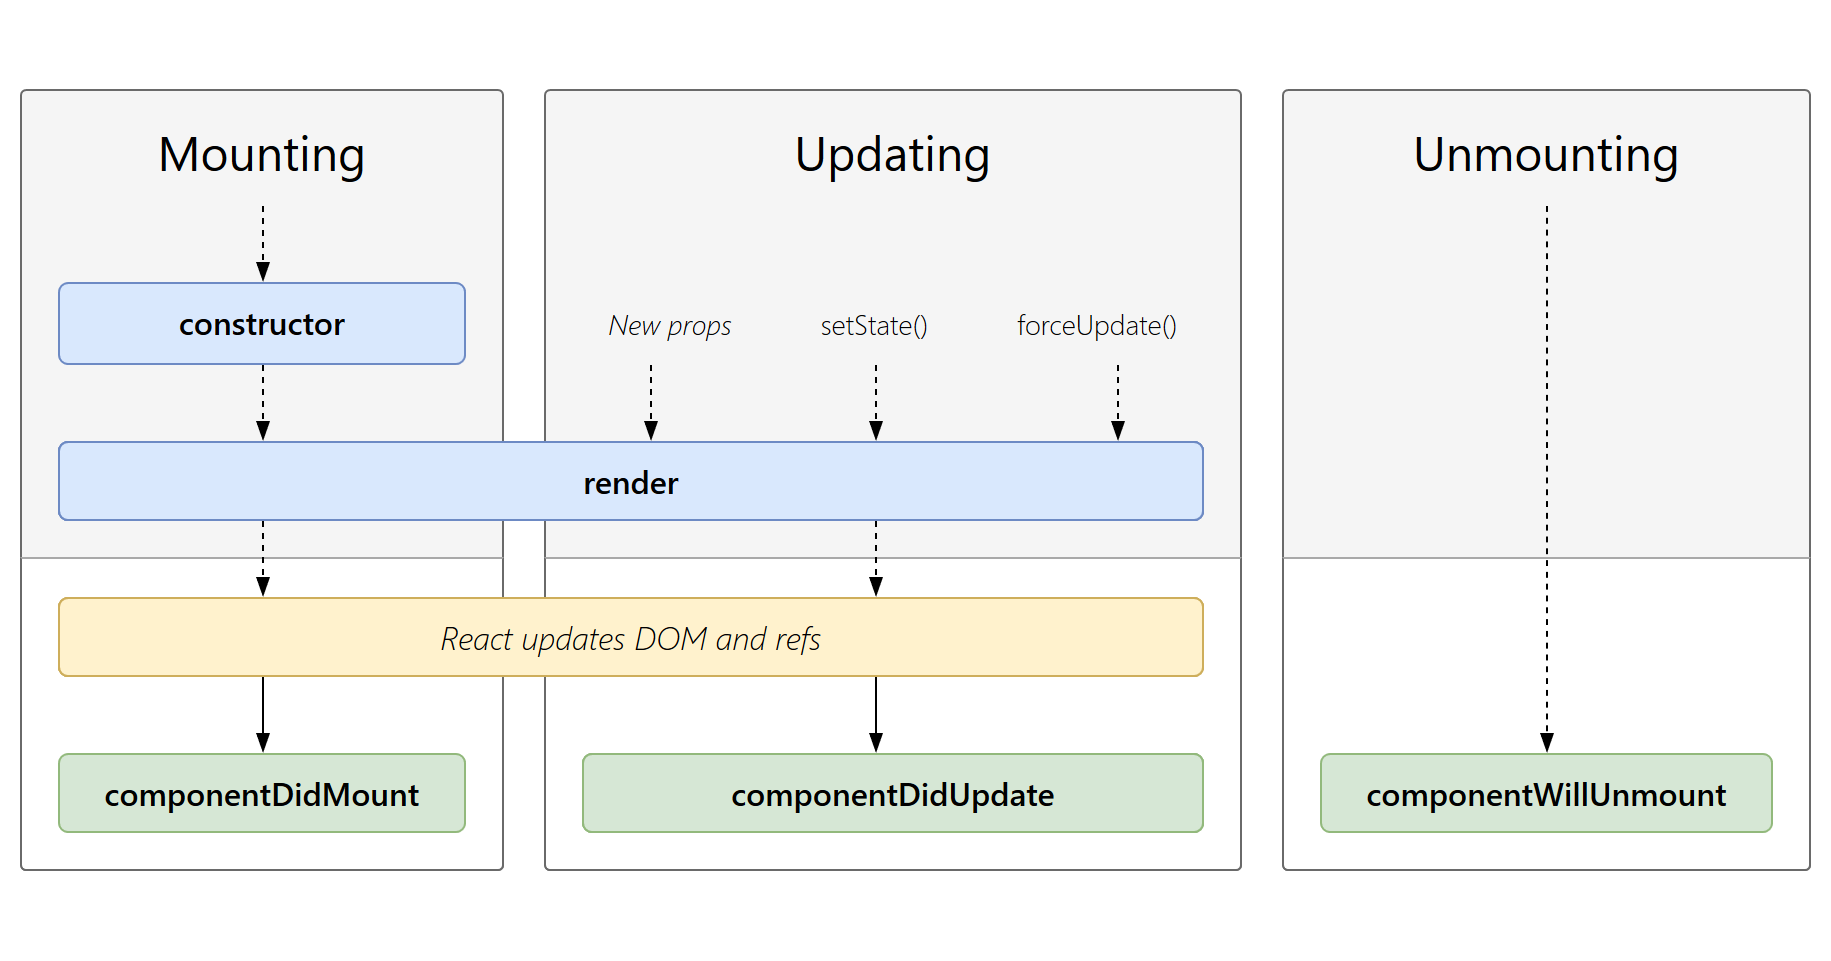
\includegraphics[width=12cm]{figure/literature/react-lifecycle.png}
                % }
                \caption[วัฏจักรการทำงานของ React]{วัฎจักรการ Render, Mount-Unmount และ Update ของ React (React Lifecycle) จาก \href{https://projects.wojtekmaj.pl/react-lifecycle-methods-diagram/}{projects.wojtekmaj.pl} }\label{fig:lit-react}
            \end{figure}
            \begin{flushleft}
                React ให้เครื่องมือและโครงสร้างที่สำหรับการสร้าง UI components ที่หลากหลายและมีประสิทธิภาพ~\cite{crockford08js} หนึ่งในข้อได้เปรียบของ React อยู่ที่การใช้ Virtual DOM ที่ช่วยเพิ่มประสิทธิภาพของการ render องค์ประกอบของ UI และการสร้างแอปพลิเคชันที่มีประสิทธิภาพและสามารถบริหารจัดการ state ของแอปพลิเคชันได้ง่าย~\cite{flanagan20js}
            \end{flushleft}
        %%%%%%%%%%%%%%%% GoFiber %%%%%%%%%%%%%%%%
        \subsubsection{GoFiber}
            \begin{flushleft}
                GoFiber เป็นเฟรมเวิร์คเบ็ดเสร็จที่เขียนขึ้นมาในภาษา Go (Golang) ที่ใช้สำหรับการพัฒนาเว็บแอปพลิเคชันแบบ high-performance พัฒนาขึ้นเพื่อเป็นตัวเลือกที่มีประสิทธิภาพสูงกว่าสำหรับเว็บแอปพลิเคชันที่ใช้งาน Go ทั่วไป โดย GoFiber ถูกออกแบบให้ง่ายต่อการใช้งานและเข้าใจ ด้วยสมรรถนะที่สูงในการดำเนินการต่าง ๆ รวมถึงการทำ Routing และการมี Middleware ต่าง ๆ ทำให้ประสิทธิภาพการทำงานของตัว GoFiber นั้นสูง~\cite{gofiber}
            \end{flushleft}
            \begin{flushleft}
                จากตัวอย่างสำหรับ demo ตัว GoFiber ที่ทำโดย \textit{Ali Y.}~\cite{ali20fiber} เเสดงให้เห็นถึงความสามารถที่โดดเด่นของ GoFiber ได้แก่ความเร็วในการทำงานที่สูง มีการจัดการ Routing ที่มีประสิทธิภาพ นอกจากนี้ GoFiber ยังมีความยืดหยุ่นในการใช้งาน Middleware และการจัดการ HTTP Context ที่เข้าใจง่าย จึงเป็นทางเลือกที่ดีสำหรับการพัฒนาเว็บแอปพลิเคชันที่ต้องการประสิทธิภาพสูงในภาษา Go
            \end{flushleft}
            \begin{flushleft}
                จากความเห็นของ \textit{Chouhan A.}~\cite{chouhan21fiber} ในบทความของเขา การใช้ GoFiber อาจมีข้อจำกัดในเบื้องต้นที่ยังไม่ครอบคลุมความสามารถทั้งหมดของภาษา Go และต้องพบกับชุดคำสั่งที่จำกัดอย่างเล็กน้อย
            \end{flushleft}
        %%%%%%%%%%%%%%%% Grafana %%%%%%%%%%%%%%%%
        \subsubsection{Grafana}
                \begin{figure}[H]
                \centering
                % \fbox{
                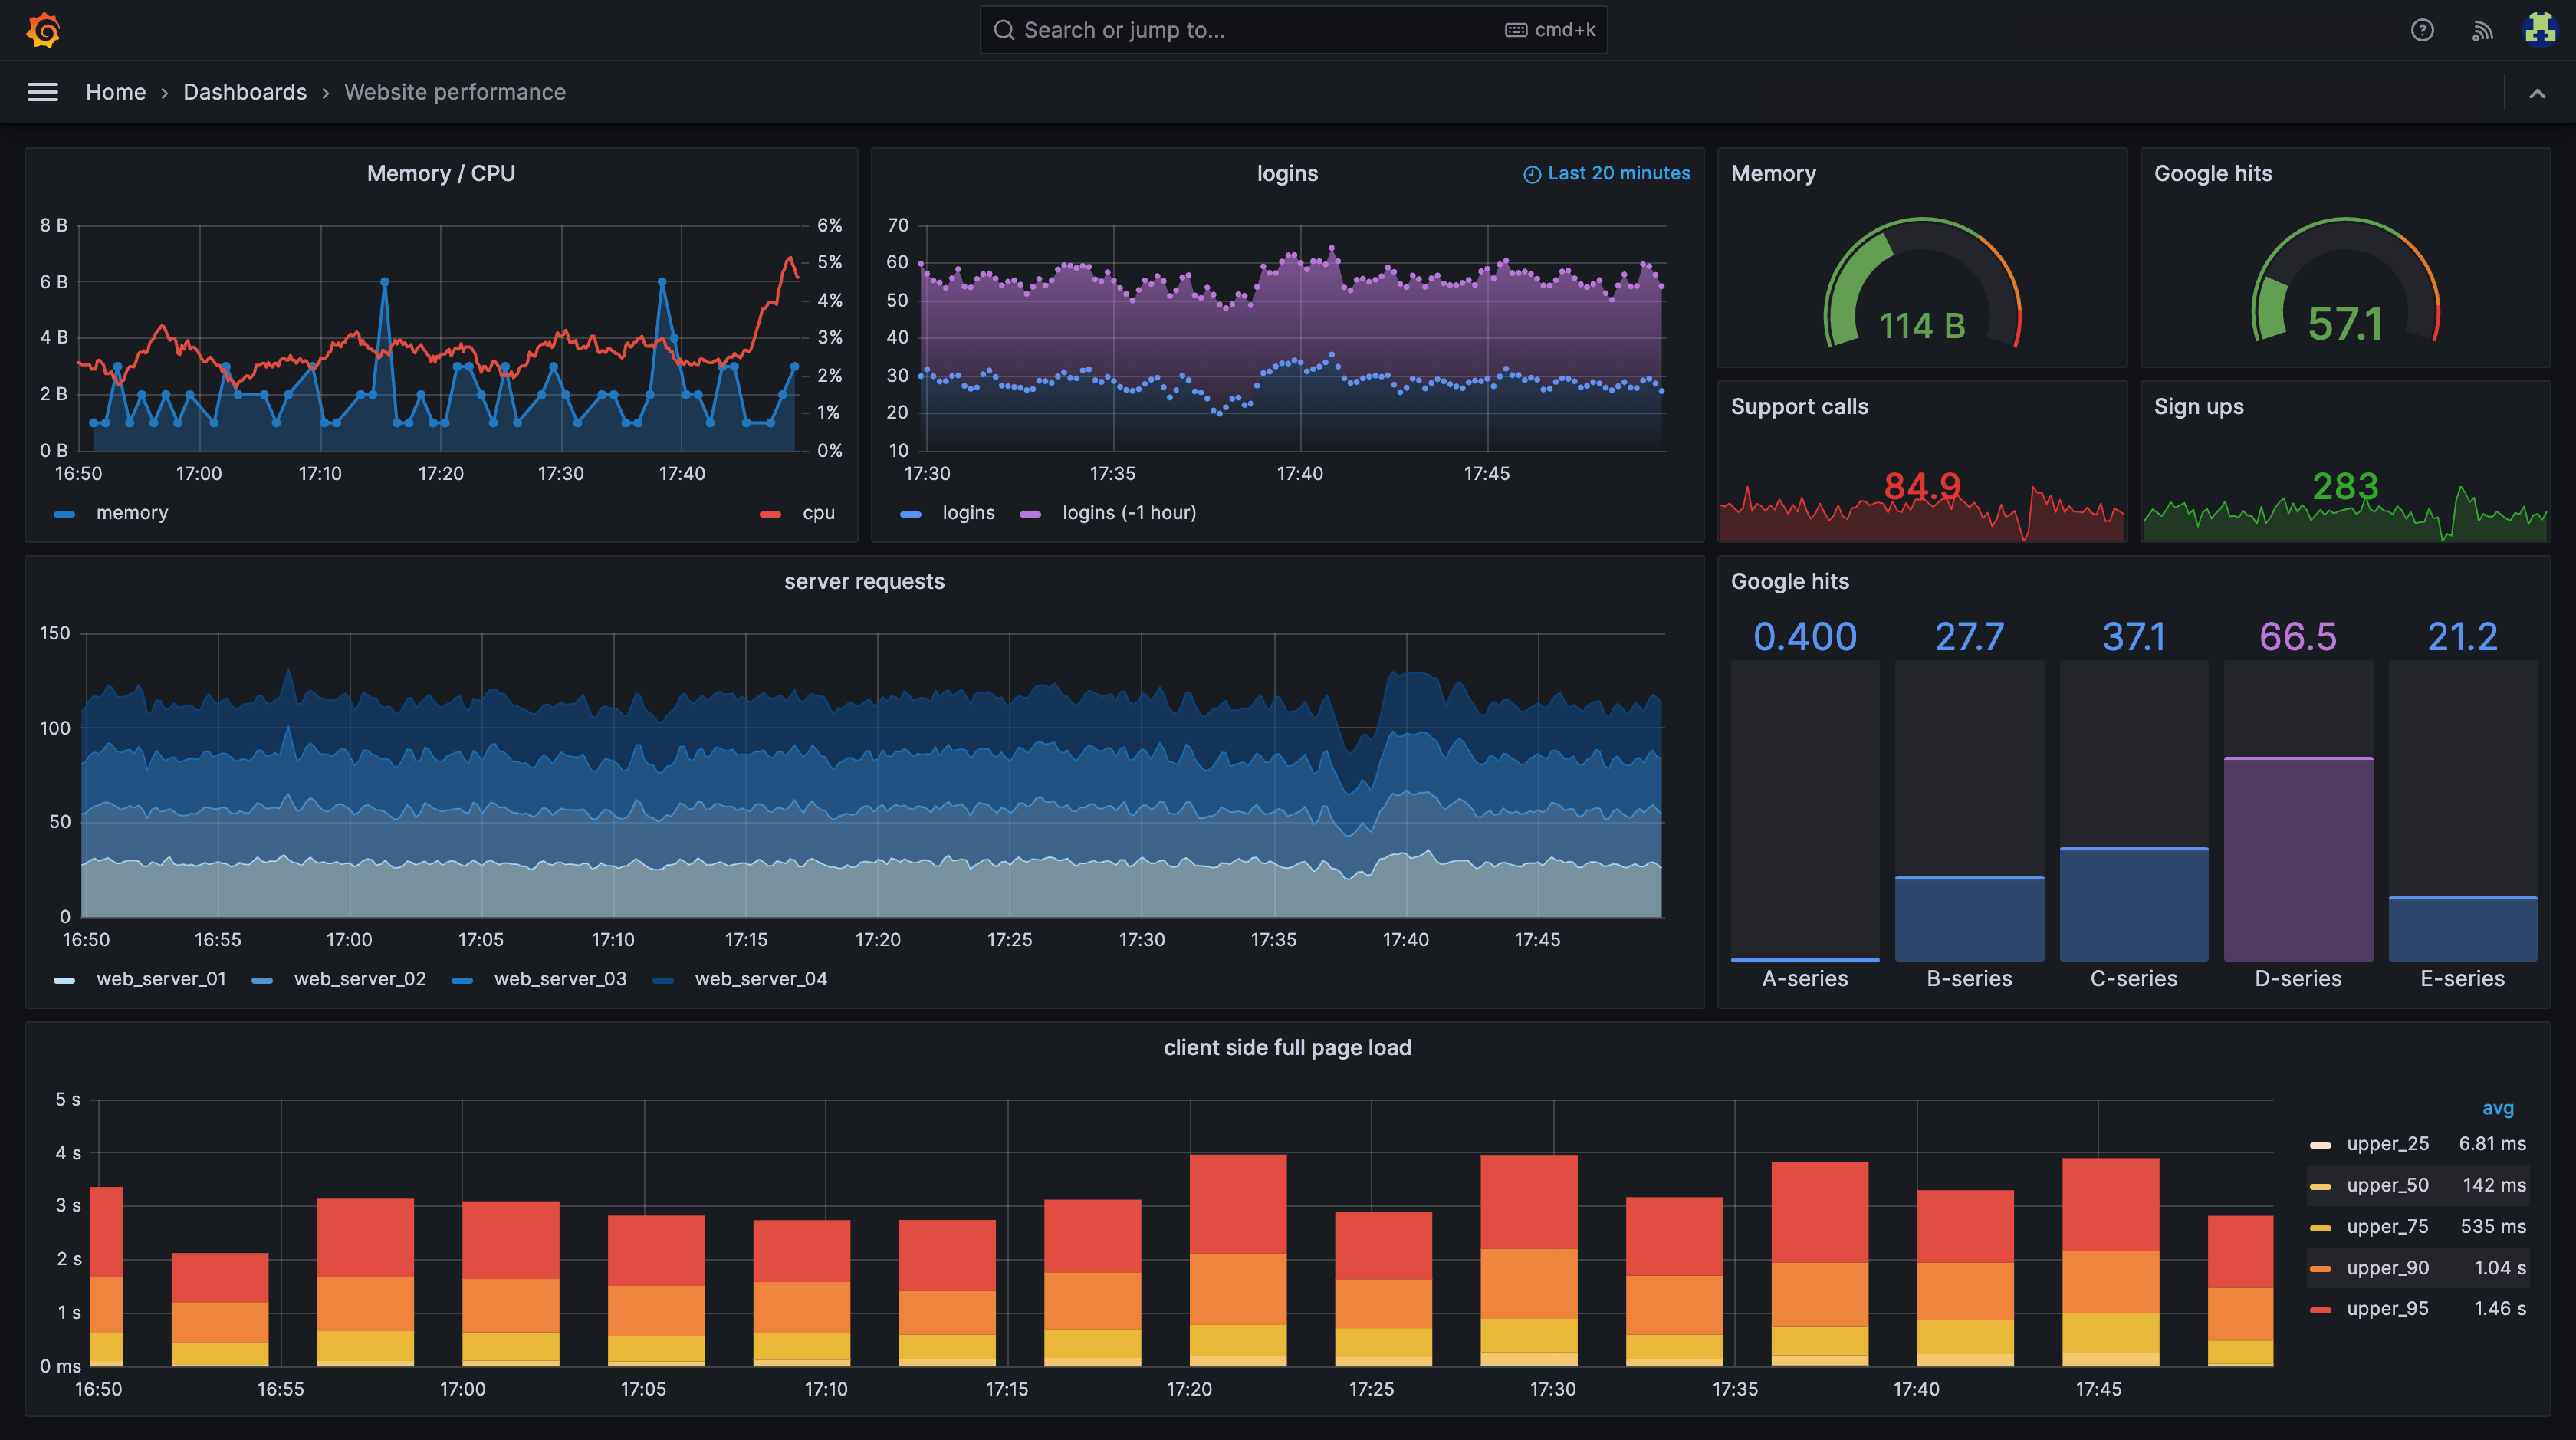
\includegraphics[width=14cm]{figure/literature/grafana.png}
                % }
                \caption[ตัวอย่างหน้าซอฟต์แวร์ Grafana]{ตัวอย่างหน้าซอฟต์แวร์ Grafana จาก \href{https://grafana.com/oss/grafana/}{หน้า Home Page ของ Grafana} }\label{fig:lit-grafana}
            \end{figure}
            \begin{flushleft}
                Grafana เป็นเครื่องมือสำหรับการแสดงผลข้อมูลแบบ Real-time และ Monitoring ที่มีความนิยมอย่างแพร่หลายในวงการ IT และพัฒนาซอฟต์แวร์ มันมีความสามารถในการเชื่อมต่อกับแหล่งข้อมูลต่าง ๆ เช่น ฐานข้อมูล, ระบบ Monitor, และ Web Services เพื่อนำข้อมูลมาแสดงผลในรูปแบบกราฟ, ตาราง, และแผนที่เพื่อให้ผู้ใช้งานสามารถวิเคราะห์และทำความเข้าใจข้อมูลได้ง่ายขึ้น~\cite{grafana}
            \end{flushleft}
            \begin{flushleft}
                Grafana นั้นมีความยืดหยุ่นสูงในการตั้งค่าและการปรับแต่งการแสดงผล ทำให้มีความสามารถที่ใหญ่ขึ้นในการปรับแต่ง Dashboard ตามความต้องการของผู้ใช้~\cite{grafana}
            \end{flushleft}
            \begin{flushleft}
                จากรายงานของ \textit{Sunil K. \& Savaranan C.}~\cite{sunil21grafana} ถึงแม้ว่าความสามารถในการสร้าง Alert และ Notification จะมีจำกัดและใช้ยาก แต่ Grafana นั้นเต็มไปด้วยฟีเจอร์อื่น ๆ มากมาย ทั้งใช้งานง่ายและมีความยืดหยุ่นสูง มี option ที่สามารถกำหนดเองได้ ทำให้แผงการแสดงภาพที่หลากหลาย ซึ่งทำให้การ Monitor หรือ Visualize ข้อมูล มีสีสันและชีวิตชีวา
            \end{flushleft}
        %%%%%%%%%%%%%%%% GitHub %%%%%%%%%%%%%%%%
        \subsubsection{GitHub}
            \begin{flushleft}
                GitHub เป็นเว็บแพลตฟอร์มที่ให้บริการ Hosting ระบบ Version Control แบบ Distributed ในรูปแบบของ Git นอกจากนี้, GitHub ยังเป็นสถานที่ที่นักพัฒนาสามารถทำงานร่วมกันและแบ่งปันโค้ดต่าง ๆ ภายใต้รูปแบบของ Repository ทำให้เป็นที่นิยมสำหรับการพัฒนาซอฟต์แวร์ Open Source และโครงการที่มีทีมพัฒนาขนาดใหญ่~\cite{github}
            \end{flushleft}
            \begin{flushleft}
                GitHub มีความสามารถในการทำงานร่วมกันในโปรเจคผ่าน Git ซึ่งมีข้อได้เปรียบในการจัดการเวอร์ชันของโค้ดและการตรวจสอบการเปลี่ยนแปลง การให้บริการ Issue Tracking และ Pull Request ทำให้งานพัฒนาไปได้อย่างมีระบบและมีความเป็นระบบ~\cite{github, chacon14}
            \end{flushleft}
            \begin{flushleft}
                แต่ GitHub มีค่าบริการสำหรับการให้บริการ Version Control แด่องค์กรหรือทีมนักพัฒนาที่สูงขึ้นเมื่อเวลาผ่านไป~\cite{githubprice}
            \end{flushleft}
        %%%%%%%%%%%%%%%% Docker %%%%%%%%%%%%%%%%
        \subsubsection{Docker}
            \begin{flushleft}
                Docker เป็นแพลตฟอร์ม Containerization ที่ช่วยให้นักพัฒนาสามารถพัฒนาและใช้งานโปรแกรมได้ง่ายขึ้น โดยไม่ต้องสนใจว่าจะทำงานบนระบบปฏิบัติการ (OS) อะไรทั้งสิ้น~\cite{docker} หลักการของการ Containerization คือการแนบ Dependencies และ Software ทั้งหมดที่ต้องใช้เข้าไปในภาชนะหรือกล่อง ๆ เดียวเป็น bundle หรือ container ทำให้สามารถเรียกใช้งานได้ทันที โดยที่ไม่ต้องติดตั้งหรือตั้งค่าเครื่อง ลงโปรแกรมหรือระบบปฏิบัติการเอง~\cite{docker, yıldız23docker} อีกทั้ง Docker มีความสามารถในการทำงานในรูปแบบ Isolation, มีการทำ Resource Optimization, และมีความ Portability ทำให้เป็นเครื่องมือที่ได้รับความนิยมในการพัฒนาและการดำเนินการระบบ~\cite{yıldız23docker}
            \end{flushleft}
            \begin{flushleft}
                Docker ช่วยลดปัญหาที่เกิดขึ้นจากความแตกต่างของระบบปฏิบัติการและสภาพแวดล้อมการทำงานระหว่าง Development และ Production โดยลดปัญหา "It works on my machine" ซึ่งก็คือปัญหาที่โปรแกรมจะทำงานในเครื่องคอมพิวเตอร์เครื่องหนึ่งแต่ไม่ทำงานในอีกเครื่องหนึ่ง~\cite{yıldız23docker} จากบทความของ \textit{Chesterwood R.}~\cite{chesterwood21microservice} Docker ยังช่วยในการปรับใช้โปรแกรมในลักษณะ Microservices Architecture ทำให้การพัฒนาและการดูแลรักษาระบบเป็นไปอย่างมีประสิทธิภาพ
            \end{flushleft}
            \begin{flushleft}
                เช่นเดียวกับเครื่องมือก่อน ๆ Docker อาจมีความซับซ้อนสูงขึ้นและเรียนรู้การใช้งานยาก ในการกำหนดค่าและจัดการ Container หลาย ๆ ตัวพร้อมกันในระบบก็๋เป็นเรื่องที่ยากและใช้ความรู้มหาศาล~\cite{dockerdoc} และจากความเห็นของ \textit{Yıldız H.}~\cite{yıldız23docker} ถึงเเม้ Docker จะเป็นซอฟต์แวร์ที่ light-weighted ในบางกรณี Docker อาจส่งผลกระทบต่อการทำงานโดยภาพรวมของระบบ System Performance หากบริหารไม่ดี
            \end{flushleft}
        %%%%%%%%%%%%%%%% Terraform %%%%%%%%%%%%%%%%
        \subsubsection{Terraform}
            \begin{flushleft}
                Terraform เป็นเครื่องมือสำหรับ Infrastructure as Code (IaC) ที่ออกแบบมาเพื่อจัดการและกำหนดค่า Infrastructure ทั้งใน Cloud และ On-Premises อย่างมีประสิทธิภาพ~\cite{terraform} ผู้ใช้สามารถใช้ภาษาที่อ่านง่ายเพื่อกำหนดค่าและสร้าง Infrastructure ที่ต้องการ เช่น Virtual Machines, Networks, Databases และ Resources อื่น ๆ ในรูปแบบของ Code~\cite{terraform} จากบทความเรื่องข้อดีของ Terraform โดย \textit{Tripathi P.}~\cite{tripathi23terraform} ได้พูดถึงข้อดีสำคัญของ Terraform หลายประการตั้งแต่ความยืดหยุ่น, ทนทาน, ไปจนถึงความสามารถในทำงานร่วมกับหลาย Cloud Provider อย่างมีประสิทธิภาพ 
            \end{flushleft}
            \begin{flushleft}
                การใช้ Terraform ช่วยลดการพิมพ์ Configuration Code ที่จะใช้กำหนดค่า Infrastructure ลงไปใน Code ของโปรเจคและช่วยในการตรวจสอบสถานะและการดำเนินการ Infrastructure อย่างทันที แต่ผู้ใช้ต้องเรียนรู้และทำความเข้าใจการใช้งาน Terraform อย่างลึกซึ้งเพื่อให้การใช้งานมีประสิทธิภาพ~\cite{stanfield22iac}
            \end{flushleft}
        %%%%%%%%%%%%%%%% Kubernetes %%%%%%%%%%%%%%%%
        \subsubsection{Kubernetes}
            \begin{flushleft}
                Kubernetes เป็นระบบ Orchestrator ที่ใช้ในการจัดการและควบคุม Containers ในรูปแบบ Cluster มีความสามารถในการปรับขยายและจัดการสถานะของ Containers ต่าง ๆ ในทันที ทำให้เป็นเครื่องมือที่ดีสำหรับการปรับใช้และการจัดการ Microservices และ Applications ที่ทำงานบน Containers อีกทั้ง Kubernetes ช่วยลดภาระงานในการสร้าง, ดูแล, และปรับขยายระบบที่มีมากถึงหลายหลาย Containers~\cite{kubernetes}
            \end{flushleft}
            \begin{flushleft}
                ความสามารถในการตรวจจับและแก้ไขข้อผิดพลาดในการทำงานของ Containers รวมถึงการปรับเปลี่ยนอัตโนมัติในกรณีที่มี Containers ล่ม ทำให้ระบบยืดหยุ่นและทนทานมากขึ้น~\cite{kubernetes} แต่เช่นเดียวกับตัว Docker เอง การจัดการ Kubernetes อาจมีความซับซ้อนและต้องการเรียนรู้การใช้งานในระดับที่สูง
            \end{flushleft}
    \subsection{โครงสร้างพื้นฐาน}
        %%%%%%%%%%%%%%%% Kubernetes %%%%%%%%%%%%%%%%
        \subsubsection{MySQL}
            \begin{flushleft}
                MySQL เป็นระบบจัดการฐานข้อมูลแบบ Relational Database Management System (RDBMS) ที่เป็น Open Source และได้รับความนิยมอย่างแพร่หลาย มีความสามารถในการจัดเก็บและจัดการข้อมูลในรูปแบบตารางที่สอดคล้องกับโครงสร้างของฐานข้อมูล~\cite{mysql} ทำให้เป็นทางเลือกที่ดีสำหรับโปรเจคที่มีโครงสร้างข้อมูลที่แน่นอน เนื่องด้วยความเป็นที่นิยมและการที่ยังมีคนใช้ประโยชน์จากตัวซอฟต์แวร์ตัสนี้อยู่ MySQL มี Community Edition ที่ให้บริการฟรีและมีการพัฒนาที่ต่อเนื่องอย่าง~\cite{mysqlcomm}
            \end{flushleft}
            %%% citation needed %%%
            \begin{flushleft}
                ข้อดีของ MySQL รวมถึงประสิทธิภาพในการค้นหาและดึงข้อมูล, รองรับการใช้งานที่หนักหน่วง, และมีความปลอดภัยในการจัดการข้อมูล แต่ก็ใช่ว่า MySQL จะเหมาะสมกับทุกโปรเตค  บางครั้ง MySQL อาจจะไม่เหมาะสมกับโปรเจคที่มีความซับซ้อนและต้องการการจัดการข้อมูลในมิติที่หลากหลาย
            \end{flushleft}
        %%%%%%%%%%%%%%%% InfluxDB %%%%%%%%%%%%%%%%
        \subsubsection{InfluxDB}
            \begin{flushleft}
                InfluxDB เป็นฐานข้อมูลแบบ Time Series Database ที่ออกแบบมาเพื่อจัดเก็บและจัดการข้อมูลที่มีการเปลี่ยนแปลงตลอดเวลา นิยมถูกใช้ในงานที่ต้องการจัดเก็บข้อมูลการวัดหรือเวลาจริง เช่น ข้อมูลเซ็นเซอร์ หรือข้อมูลการทดสอบและข้อมูลการวิเคราะห์จากต้นทางที่ส่งมาพร้อมเวลา timestamp~\cite{influxdb} มีความยืดหยุ่นและสามารถทำงานร่วมกับหลายแพลตฟอร์ม~\cite{influxdb-platforms}
            \end{flushleft}
            %%%% citation needed %%%
            \begin{flushleft}
                ความเร็วในการทำงานและการดึงข้อมูลใน InfluxDB เป็นจุดเด่นที่สำคัญ โดยเฉพาะเมื่อมีความต้องการในการจัดเก็บและดึงข้อมูลจำนวนมากในช่วงเวลาที่สั้น แต่ก็อาจมีข้อจำกัดในการจัดเก็บข้อมูลที่ไม่ใช่ Time Series และการรองรับขนาดข้อมูลที่ใหญ่
            \end{flushleft}
        %%%%%%%%%%%%%%%% Prometheus %%%%%%%%%%%%%%%%
        \subsubsection{Prometheus}
            \begin{flushleft}
                Prometheus เป็นระบบการตรวจสอบและติดตาม (monitoring and alerting) ที่ถูกออกแบบมาสำหรับระบบที่มีโครงสร้างที่ยืดหยุ่นและต้องการการดูแลที่ส่วนตัว~\cite{prometheus} มีความสามารถในการเก็บข้อมูลและวิเคราะห์ข้อมูลเพื่อตรวจสอบปัญหาและเป็นเครื่องมือที่มีประสิทธิภาพในการจัดการระบบที่ใหญ่ 
            %%% citation needed %%%
            \begin{flushleft}
                Prometheus มีการส่งเสริมการใช้งานร่วมกับ Kubernetes และมีการส่งเสริมที่ดีในการใช้งานที่แพร่หลายในระบบคลาวด์
            \end{flushleft}
            \end{flushleft}
            %%% citation needed %%%
            \begin{flushleft}
                ความยืดหยุ่นและการติดตามเหตุการณ์ในเวลาที่เป็นเรียลไทม์เป็นจุดเด่นสำคัญของ Prometheus, ทำให้เป็นเครื่องมือที่เหมาะสมสำหรับการค้นหาและแก้ไขปัญหาที่เกิดขึ้นทันที แต่ในระบบที่มีขนาดใหญ่และต้องการการเก็บข้อมูลที่ยาวนาน แต่พื้นที่เก็บข้อมูลของ Prometheus อาจมีความจำกัดและข้อมูลอาจล้นเกินได้
            \end{flushleft}

        %%%%%%%%%%%%%%%% RabbitMQ %%%%%%%%%%%%%%%%
        \subsubsection{RabbitMQ}
            \begin{flushleft}
                RabbitMQ เป็นระบบ Message Broker ที่มีคุณสมบัติและบริการในการจัดการและส่งข้อมูลระหว่างแอปพลิเคชันต่าง ๆ~\cite{rabbitmq} ในรูปแบบที่มีประสิทธิภาพ ด้วยความที่ซอฟต์แวร์เป็น Open Source ทำให้ได้รับความนิยมเป็นอย่างสูง ได้ถูกนำมาใช้การทำงานในสภาพแวดล้อมที่ต้องการการกระจายข้อมูลและการคอมมูนิเคชัน อีกทั้งการใช้ RabbitMQ ช่วยลดความซับซ้อนในการสื่อสารระหว่างบริการและแอปพลิเคชัน, ทำให้ระบบสามารถทำงานได้อย่างยืดหยุ่นและมีประสิทธิภาพ~\cite{rabbitmq}
            \end{flushleft}
            %%% citation required verification %%%
            \begin{flushleft}
                ความยืดหยุ่นของ RabbitMQ ทำให้เป็นเครื่องมือที่มีประสิทธิภาพสำหรับการทำ Message Queue และการจัดการกับการแลกเปลี่ยนข้อมูลที่ต้องการการทำงานแบบอนุกรม~\cite{videla17rabbitmq} ในเเง่ของข้อเสียการดูแลรักษาและบริหารจัดการ RabbitMQ ในสภาพแวดล้อมที่มีใช้งานการสื่อสารมาก ๆ อาจมีความซับซ้อน~\cite{hanwell17rabbitmq}
            \end{flushleft}   
\pagebreak
%%%%%%%%%%%%%%%%%%%%%%%%%%%%%%%%%%%%%%%%%%%%%%%%%%%%%
%%%%%%%%%% Design and Methodologies %%%%%%%%%%%%%%%%%
%%%%%%%%%%%%%%%%%%%%%%%%%%%%%%%%%%%%%%%%%%%%%%%%%%%%%
\chapter{วิธีการดำเนินงาน}

% \emph{หัวข้อต่าง ๆ ในแต่ละบทเป็นเพียงตัวอย่างเท่านั้น หัวข้อที่จะใส่ในแต่ละบทขึ้นอยู่กับโปรเจคของนักศึกษาและอาจารย์ที่ปรึกษา}

% ตัวอย่างการใส่อ้างอิงที่มา -> \cite{hypersense} ถ้าต้องการใส่แหล่งอ้างอิงมากกว่า 1 ให้ทำดังนี้ -> \cite{hypersense,bworld} 
% Explain the design (how you plan to implement your work) of your project. Adjust the section titles below to suit the types of your work. Detailed physical design like circuits and source codes should be placed in the appendix.

\begin{flushleft}
ในบทที่ 3 จะกล่าวถึงภาพรวมของซอฟต์แวร์ของโครงงาน โครงสร้างระบบที่ทางคณะผู้จัดทำโครงการได้วางเอาไว้ ลักษณะฐานข้อมูลที่ใช้ในการจัดเก็บข้อมูล การใช้งานระหว่างระบบออกแบบมาตอบโจทย์ผู้ใช้งาน รวมไปถึงการจัดการภายในระบบที่ได้ออกแบบไว้อย่างดี
\end{flushleft}
\begin{flushleft}
สถาปัตยกรรมระบบที่ได้วางไว้ มีความเป็นระเบียบและเหมาะสม ระบบฐานข้อมูลก็ออกแบบมาให้เรียบง่าย ผสมผสานกับการใช้เทคโนโลยีที่เหมาะสมและทันสมัย ทางคณะผู้จัดทำโครงการ เชื่อมั่นว่าซอฟต์แวร์ที่ออกแบบมา จะสามารถทำงานอย่างมีประสิทธิภาพ ประมวลผลเร็ว
\end{flushleft}
\begin{flushleft}
จากสถาปัตยกรรมระบบที่ได้ออกแบบไว้ใน\hyperlink{arch-sec}{หัวข้อสถาปัตยกรรมระบบ} การใช้ตัวประสานงาน (หรือ “nginx ingress” ในรูปที่~\ref{fig:arch}) ระหว่างฝั่งผู้ใช้ (Client) กับระบบ จะสามารถแบ่งเบาและแจกจ่ายคำขอจากผู้ใช้อย่างมีประสิทธิภาพ และอีกทั้งการใช้ตัวสื่อสาร (Message Broker หรือ “RabbitMQ” ในรูปที่~\ref{fig:arch}) ระหว่างตัวซอฟต์แวร์หลักกับตัวโมดูลตรวจงานเขียนโปรแกรม (Grading Core) จะทำให้การจัดการคิวคำขอตรวจงานเขียนโปรแกรมง่ายขึ้น  ทำให้การตรวจให้คะแนน ประกาศผลคะแนนและบันทึกลงฐานข้อมูล ดำเนินการตามลำดับอย่างต่อเนื่อง
\end{flushleft}
\begin{flushleft}
จากเหตุผลข้างต้น ในเชิงอดุมคติ ซอฟต์แวร์ที่ทางกลุ่มผู้จัดทำโครงการออกแบบมาจะสามารถรับมือกับคำขอจากฝั่งผู้ใช้ได้จำนวนมหาศาล รองรับจำนวนผู้ใช้เข้ามาใช้งานในระบบพร้อมกันได้จำนวนมาก
\end{flushleft}

\section{รายละเอียดของโครงงาน}
    \subsection{ข้อกำหนดและความต้องการของระบบ}
    
    ในส่วนนี้ จะกล่าวถึงข้อกำหนดของซอฟต์แวร์หรือ User Requirements ซึ่งประกอบด้วยการทำงานในส่วนต่าง ๆ แยกประเภทเป็นตามหมวดหมู่ผู้ใช้ดังนี้ เจ้าของระบบหรือผู้ดูแลระบบ (Admin), เจ้าของห้องเรียน เจ้าของกลุ่มเรียนหรืออาจารย์ผู้สอน (Owner), ผู้ช่วยเจ้าของห้องหรือผู้ช่วยสอน (Moderator), นักศึกษา (Student), ผู้เข้าร่วมกิจกรรมหรือการแข่งขันฯ (Attendee), ผู้ใช้ทั่วไป (Registered User) และบุคคลทั่วไปหรือบุคคลภายนอก (Guest User)


    %%%%%%%%%%% SOFTWARE REQUIREMENT TABLE %%%%%%%%%%%
        \begin{table}[!h]
        \centering
        \caption{ข้อกำหนดของซอฟต์เเวร์ (1)}\label{tbl:soft-req1}
            \begin{tabular}{p{3cm}|ccccccc} \hline\hline
            Feature & Guest User & Registered User &  Student & Attendee & Moderator & Owner & Admin \\ \hline\hline
            เข้าสู่ระบบ & \checkmark & \checkmark & \checkmark & \checkmark & \checkmark & \checkmark & \checkmark \\ \hline
            ออกจากระบบ & & \checkmark & \checkmark & \checkmark & \checkmark & \checkmark & \checkmark \\ \hline
            กู้รหัสผ่าน & \checkmark & \checkmark & \checkmark & \checkmark & \checkmark & \checkmark & \checkmark \\ \hline
            ดูข้อมูลส่วนตัว  & & \checkmark & \checkmark & \checkmark & \checkmark & \checkmark & \checkmark \\ \hline
            แก้ไขข้อมูลส่วนตัว & & \checkmark & \checkmark & \checkmark & \checkmark & \checkmark & \checkmark \\ \hline
            เข้าร่วมห้องหรือกลุ่มเรียน & & \checkmark & \checkmark & \checkmark & \checkmark & \checkmark & \checkmark \\ \hline
            \end{tabular}   
    \end{table}
    \pagebreak

    \begin{table}[!h]
        \centering
        \caption{ข้อกำหนดของซอฟต์เเวร์ (2)}\label{tbl:soft-req2}
            \begin{tabular}{p{3cm}|ccccccc} \hline\hline
            Feature & Guest User & Registered User &  Student & Attendee & Moderator & Owner & Admin \\ \hline\hline
            ดูรายการห้องที่ได้เข้าร่วมทั้งหมด & & & \checkmark & \checkmark & \checkmark & \checkmark & \checkmark \\ \hline
            ดูโจทย์และภาระงานในห้องที่ได้เข้าร่วม & & & \checkmark & \checkmark & \checkmark & \checkmark & \checkmark \\ \hline
            เขียนโปรแกรมบนแอปพลิเคชัน & & & \checkmark & \checkmark & \checkmark & \checkmark & \checkmark \\ \hline
            เขียนโปรแกรมบนแอปพลิเคชัน & & & \checkmark & \checkmark & \checkmark & \checkmark & \checkmark \\ \hline
            ส่งไฟล์โปรแกรมเข้าตรวจบนแอปพลิเคชัน & & & \checkmark & \checkmark & \checkmark & \checkmark & \checkmark \\ \hline
            ดูรายการการส่งไฟล์โปรแกรมทั้งหมด & & & \checkmark & \checkmark & \checkmark & \checkmark & \checkmark \\ \hline
            ดูข้อความเห็น/คำแนะนำ/คำติชมของรายการส่งไฟล์นั้น ๆ & & & \checkmark & \checkmark & \checkmark & \checkmark & \checkmark \\ \hline
            ดูผลการตรวจและรายละเอียดของรายการส่งไฟล์โปรแกรมนั้น ๆ & & & \checkmark & \checkmark & \checkmark & \checkmark & \checkmark \\ \hline
            ดูตารางคะแนนผ่านลิงก์แชร์ & \checkmark & \checkmark & \checkmark & \checkmark & \checkmark & \checkmark & \checkmark \\ \hline
            ดูตารางคะแนนในห้องที่ได้เข้าร่วม  & & & \checkmark & \checkmark & \checkmark & \checkmark & \checkmark \\ \hline
            สามารถที่จะดูข้อมูลห้องเก่าที่เคยได้เข้าร่วม & \checkmark & \checkmark & \checkmark & \checkmark & \checkmark & \checkmark & \checkmark \\ \hline
            สามารถที่จะดูโจทย์และภาระงาน ประวัติการใช้งาน ข้อมูลของห้องเก่าที่เคยได้เข้าร่วม & \checkmark & \checkmark & \checkmark & \checkmark & \checkmark & \checkmark & \checkmark \\ \hline
            สร้างโจทย์และภาระงานในห้อง & & & & & \checkmark & \checkmark & \checkmark \\ \hline
            แก้ไขหรือจัดการโจทย์และภาระงานในห้อง & & & & & \checkmark & \checkmark & \checkmark \\ \hline
            ส่งข้อความเห็น/คำแนะนำ/คำติชมของรายการส่งไฟล์นั้น ๆ & & & & & \checkmark & \checkmark & \checkmark \\ \hline\hline
            \end{tabular}   
    \end{table}
    \pagebreak
    
    \newpage
    \subsection{กรณีการใช้งาน (Use Cases)}
    %%%%%%%%%%% USECASE DIAGRAM %%%%%%%%%%%
    \hypertarget{usecase}{
        \begin{figure}[!h]
        \centering
        % \fbox{
            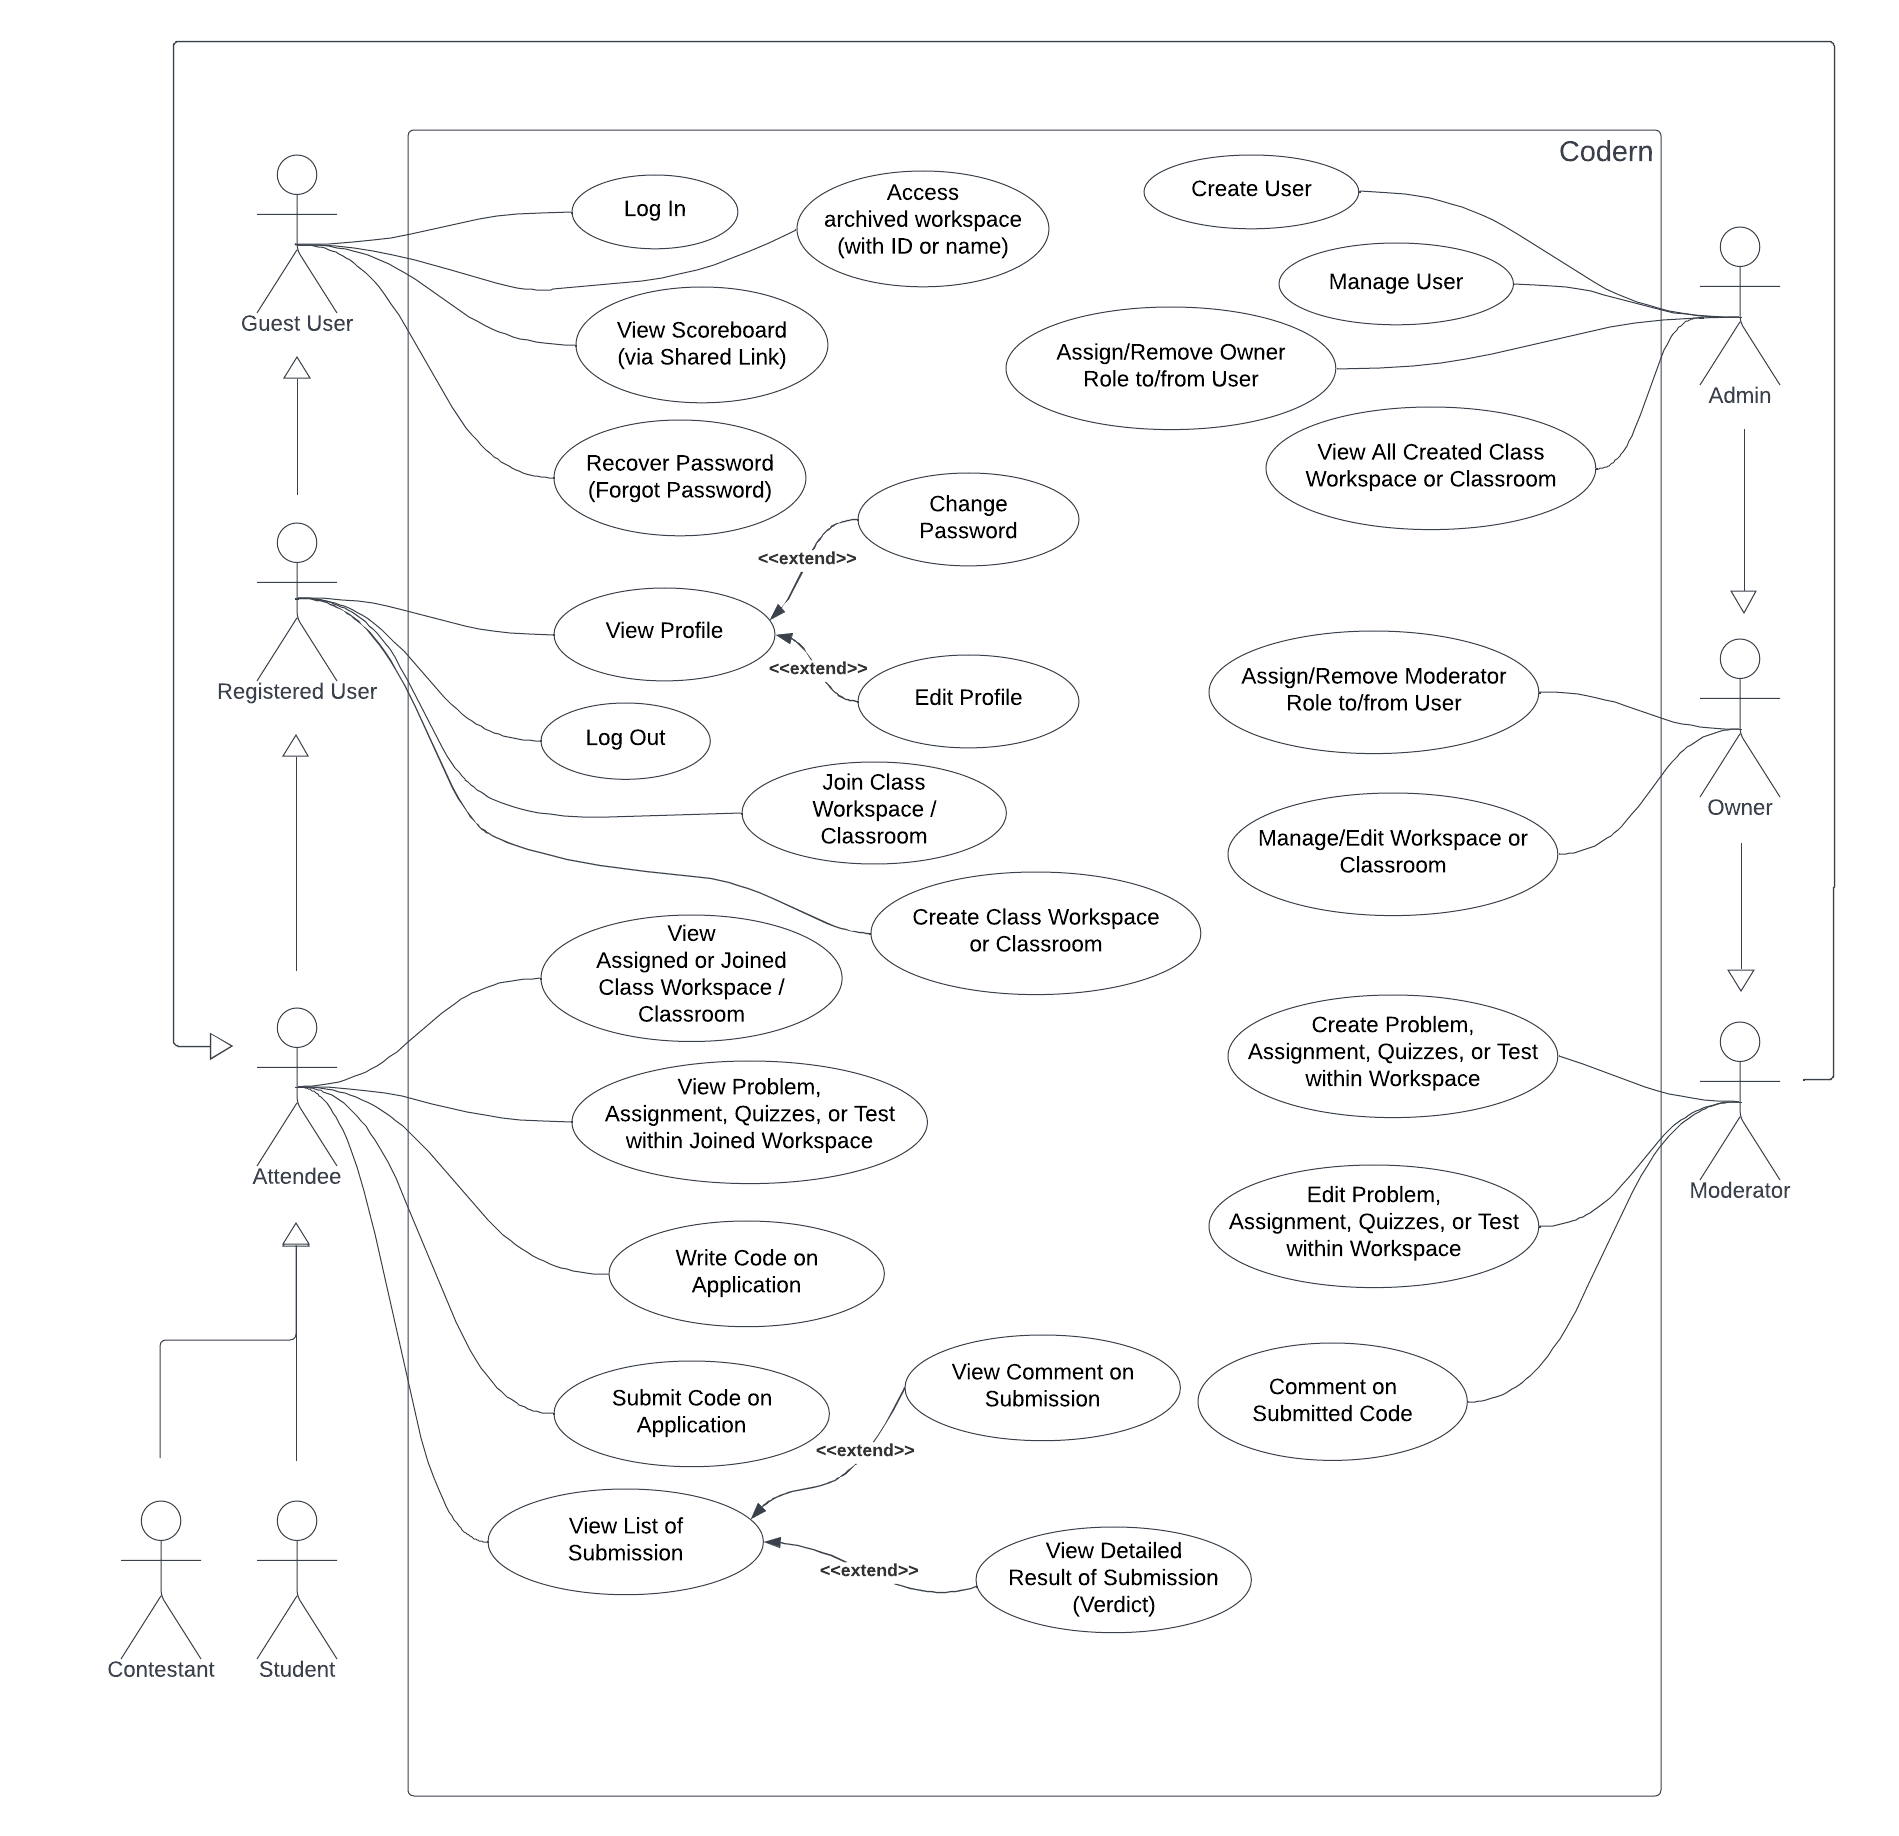
\includegraphics[width=15cm]{figure/diagram/usecase-v4.png}
        % }
        \caption[ภาพเเผนผังกรณีใช้งาน]{ภาพเเผนผังกรณีใช้งาน วาดด้วย \href{https://lucid.app/}{LucidChart} อ่านคำบรรยายได้เพิ่มเติมได้ใน\hyperlink{usecase-narrates}{หัวข้อถัดไป}}\label{fig:usecase}
        \end{figure}
    }
    \pagebreak

    \hypertarget{usecase-narrates}{\subsection{คำบรรยายกรณีใช้งาน (Use Cases Narratives)}}
    จากรูปที่~\ref{fig:usecase} ในหัวข้อที่แล้ว เป็นรูปที่แสดงความสัมพันธ์ระหว่างผู้ใช้งานและซอฟต์แวร์ ในโครงงานซอฟต์แวร์นี้ได้แบ่งประเภทผู้ใช้ออกเป็น 6 ประเภท ได้แก่บุคคลทั่วไป (Guest User), ผู้ใช้ทั่วไป (Registered User), นักศึกษา (Student), ผู้เข้าร่วมกิจกรรมหรือการแข่งขันฯ (Attendee), เจ้าของห้องหรืออาจารย์ผู้สอน (Owner), ผู้ช่วยเจ้าของห้องหรือผู้ช่วยสอน (Moderator) และเจ้าของระบบหรือผู้ดูแลระบบ (Admin)
    โดยแต่ละประเภทผู้ใช้งานมีเป้าหมายหลัก และกรณีการใช้งานดังต่อไปนี้

        \subsubsection{Guest User (บุคคลทั่วไป)}
        บุคคลทั่วไป สามารถเข้าใช้งาน feature พื้นฐานของซอฟต์แวร์ได้ดังนี้
        \begin{enumerate}
            \item “Log In” คือ การล็อกอินเข้าสู่ระบบ
            \item “View Scoreboard (via Shared Link)” คือ การเข้าถึงตารางคะแนนด้วยลิงก์ที่ถูกแชร์มา
            \item “Recover Password” คือ การกู้คืนรหัสผ่าน กรณีที่หลงลืมหรือสูญหาย
            \item “Access Archived Workspace (with ID or Name)” คือ การเข้าถึงห้องเรียน กลุ่มเรียนเก่าที่ผู้ใช้เคยได้เข้าร่วม ที่ได้ถูกเก็บรักษาไว้ (archived) ผ่านการค้นด้วยรหัสหรือชื่อ
        \end{enumerate}
    
        \subsubsection{Registered User (ผู้ใช้ทั่วไป)}
        ผู้ใช้ทั่วไปก็คือบุคคลทั่วไปที่มีบัญชีในระบบ (Admin อาจได้สร้างไว้ให้ หรือไม่ก็สมัครเอง) โดยผู้ใช้ทั่วไปสามารถเข้าถึง feature พื้นฐานของซอฟต์แวร์ได้เหมือนกับบุคคลทั่วไป (Guest User) และยังสามารถเข้าใช้ feature เพิ่มเติมได้ดังต่อไปนี้
        \begin{enumerate}
            \item “View Profile” คือ การเข้าดูข้อมูลส่วนตัวของตัวผู้ใช้เอง
            \item “Change Password” คือ การที่สามารถจะเปลี่ยนรหัสผ่านบัญชีตนเองได้
            \item “Edit Profile” คือ การที่สามารถจะแก้ไขข้อมูลส่วนตัวของบัญชีตนเองได้
            \item “Join Workspace” คือ การที่สามารถจะเข้าร่วมกลุ่มเรียน ห้องเรียนเองได้
            \item “Log Out” คือ การล็อกเอ้าท์ ออกจากระบบ
            \item “Create Class Workspace or Classroom” คือ การที่สามารถจะสร้างห้องเรียนหรือกลุ่มเรียนได้
        \end{enumerate}
        
        \subsubsection{Attendee (ผู้เข้าร่วมกิจกรรม)}
        ผู้เข้าร่วมกิจกรรมก็คือผู้ใช้ทั่วไปที่ได้เข้าร่วมห้องเรียนหรือกลุ่มเรียน (หรือ Workspace) อย่างน้อยหนึ่งห้อง สามารถเข้าถึง feature พื้นฐานของซอฟต์แวร์ได้เหมือนกับผู้ใช้ทั่วไป (Registered User) และยังสามารถเข้าใช้ feature เพิ่มเติมได้ดังต่อไปนี้
        \begin{enumerate}
            \item “View Assigned or Joined Class Workspace / Classroom” คือ การเข้าถึงรายการห้องเรียน กลุ่มเรียนทั้งหมด ที่ได้เข้าร่วมหรือถูกยัดเข้า
            \item “View Problems, Assignments, Quizzes, or Tests with Joined Workspace” คือการเข้าถึงโจทย์ปัญหา ภาระงานและข้อสอบทั้งหมดในกลุ่มเรียนหรือห้องเรียนที่ได้เข้าร่วมหรือถูกยัดเข้า
            \item “Write Code on Application” คือ การที่สามารถจะเขียนโปรแกรมบนตัวซอฟต์แวร์ได้
            \item “Submit Code on Application” คือ การที่สามารถจะส่งโปรแกรมให้ซอฟต์แวร์ไปตรวจ
            \item “View List of Submission” คือ การเข้าถึงรายการที่แสดงการส่งโปรแกรมให้ซอฟต์แวร์ไปตรวจ ที่ตัวนักศึกษาหรือผู้เข้าร่วมกิจกรรม/การแข่งขันฯ เป็นคนส่งทั้งหมด
            \item “View Comment on Submission” คือ การเข้าถึงข้อความคิดเห็น คำแนะนำ คำติชมเกี่ยวกับงานเขียนโปรแกรมที่ได้ส่งไป ที่อาจารย์ผู้สอน ผู้ช่วยสอนได้พิมพ์เอาไว้ ในการส่งโปรแกรมที่ส่งตรวจครั้งนั้น ๆ
            \item “View Detailed Result of Submission (Verdict)” คือ การเข้าถึง รายละเอียดและผลตรวจแบบละเอียดของโปรแกรมที่ส่งตรวจในแต่ละครั้ง
        \end{enumerate}
        
        \subsubsection{Student (นักเรียนหรือนักศึกษา)}
        นักเรียนหรือนักศึกษา ก็คือผู้เข้าร่วมกิจกรรมที่ได้เข้าร่วม (joined) หรือถูกยัดเข้า (assigned) ห้องเรียน กลุ่มเรียน (workspace) ดังนั้นนักเรียนหรือนักศึกษาก็จะเข้าถึง feature พื้นฐานของซอฟต์แวร์ได้เหมือนกับผู้เข้าร่วมกิจกรรม (Attendee) เหมือนกันหมดทุกประการ

        \subsubsection{Contestant (ผู้เข้าร่วมการแข่งขัน)}
        ผู้เข้าร่วมการแข่งขัน ก็คือผู้เข้าร่วมกิจกรรมที่ได้เข้าร่วม (joined) หรือถูกยัดเข้า (assigned) ห้องเรียน กลุ่มเรียน (workspace) เช่นเดียวกัน ดังนั้นผู้เข้าร่วมการแข่งขันเข้าถึง feature พื้นฐานของซอฟต์แวร์ได้เหมือนกับผู้เข้าร่วมกิจกรรม (Attendee) เหมือนกันหมดทุกประการ หรือได้ feature เทียบเท่ากับนักเรียนหรือนักศึกษา
        
        \subsubsection{Moderator (ผู้ช่วยเจ้าของห้องหรือผู้ช่วยสอน)}
        ผู้ช่วยเจ้าของห้องหรือผู้ช่วยสอน เป็นผู้ใช้ที่ถูกเจ้าของห้องหรืออาจารย์ผู้สอนหรือเจ้าระบบแต่งตั้งให้มาเป็นผู้ช่วยบริหารห้องเรียนหรือกลุ่มเรียน ผู้ใช้หมวดหมู่นี้สามารถเข้าถึง feature ของซอฟต์แวร์ได้เหมือนกับนักศึกษาหรือผู้เข้าแข่งขันฯ (Student or Attendee) แต่ก็เข้าถึง feature เพิ่มเติมได้ดังนี้
        \begin{enumerate}
            \item “Create Problems, Assignments, Quizzes, or Test within Workspace” คือ การที่สามารถสร้างโจทย์ปัญหา ภาระงานและออกข้อสอบภายในห้องเรียน หรือกลุ่มเรียนที่ตนได้คุมอยู่ได้
            \item “Edit Problems, Assignments, Quizzes, or Test within Workspace” คือ การที่สามารถจะแก้ไขโจทย์ปัญหา ภาระงานและออกข้อสอบภายในห้องเรียน หรือกลุ่มเรียนที่ตนได้คุมอยู่ได้
            \item “Comment on Submitted Code” คือ การที่สามารถจะให้ความเห็น ให้คำแนะนำหรือให้คำติชม แก่งานเขียนโปรแกรมที่นักศึกษา หรือผู้เข้าร่วมการแข่งขันฯ ได้ส่งเข้ามาในระบบได้
        \end{enumerate}
        
        \subsubsection{Owner (เจ้าของห้องหรืออาจารย์ผู้สอน)}
        เจ้าของห้องหรืออาจารย์ผู้สอน คือผู้ใช้ที่สามารถสร้างและบริหารจัดการห้องเรียนหรือกลุ่มเรียนได้ ผู้ใช้หมวดหมู่นี้สามารถเข้าถึง feature ของซอฟต์แวร์ได้เหมือนกับผู้ช่วยเจ้าของห้อง (Moderator) และเข้าถึง feature เพิ่มเติมได้ดังนี้
        \begin{enumerate}
            \item “Assign/Remove Moderator Role to/from User” คือ ความสามารถที่จะแต่งตั้งหรือลดบทบาทผู้ใช้ทั่วไปให้มาเป็นผู้ช่วยสอนหรือผู้ช่วยเจ้าของห้อง (moderator)
            \item “Manage or Edit Workspace or Classroom” คือ ความสามารถที่จะแก้ไข บริหารจัดการ (ลบ) ห้องเรียนหรือกลุ่มเรียนทั้งหมดที่ตนเป็นเจ้าของ
        \end{enumerate}
        
        \subsubsection{Admin (เจ้าของระบบหรือแอดมิน)}
        เจ้าของระบบหรือแอดมิน สามารถเข้าถึง feature ของซอฟต์แวร์ได้เหมือนกับเจ้าของห้องหรืออาจารย์ผู้สอน (Owner) แต่เข้าถึง feature พิเศษเพิ่มเติมได้ ดังนี้
        \begin{enumerate}
            \item “Create User” คือ ความสามารถในการสร้างบัญชีผู้ใช้ได้
            \item “Manage User” คือ การที่สามารถที่จะบริหารจัดการ (ลบ) ข้อมูลบัญชีผู้ใช้ทั้งหมดได้
            \item “Assign/Remove Owner Role to/from User” คือ ความสามารถที่จะแต่งตั้งหรือลดบทบาทผู้ใช้ ให้มาเป็นเจ้าของห้อง (owner)
            \item “View All Created Class Workspace or Classroom” คือ การเข้าถึงรายการแสดงผลห้องเรียนหรือกลุ่มเรียนทั้งหมดที่ได้สร้างขึ้นในระบบ
        \end{enumerate}
    \pagebreak
    
\hypertarget{arch-section}{\section{สถาปัตยกรรมระบบ}}
    %%%%%%%%%%% ARCHITECTURE DIAGRAM %%%%%%%%%%%
    \begin{figure}[!h]
    \centering
    % \fbox{
        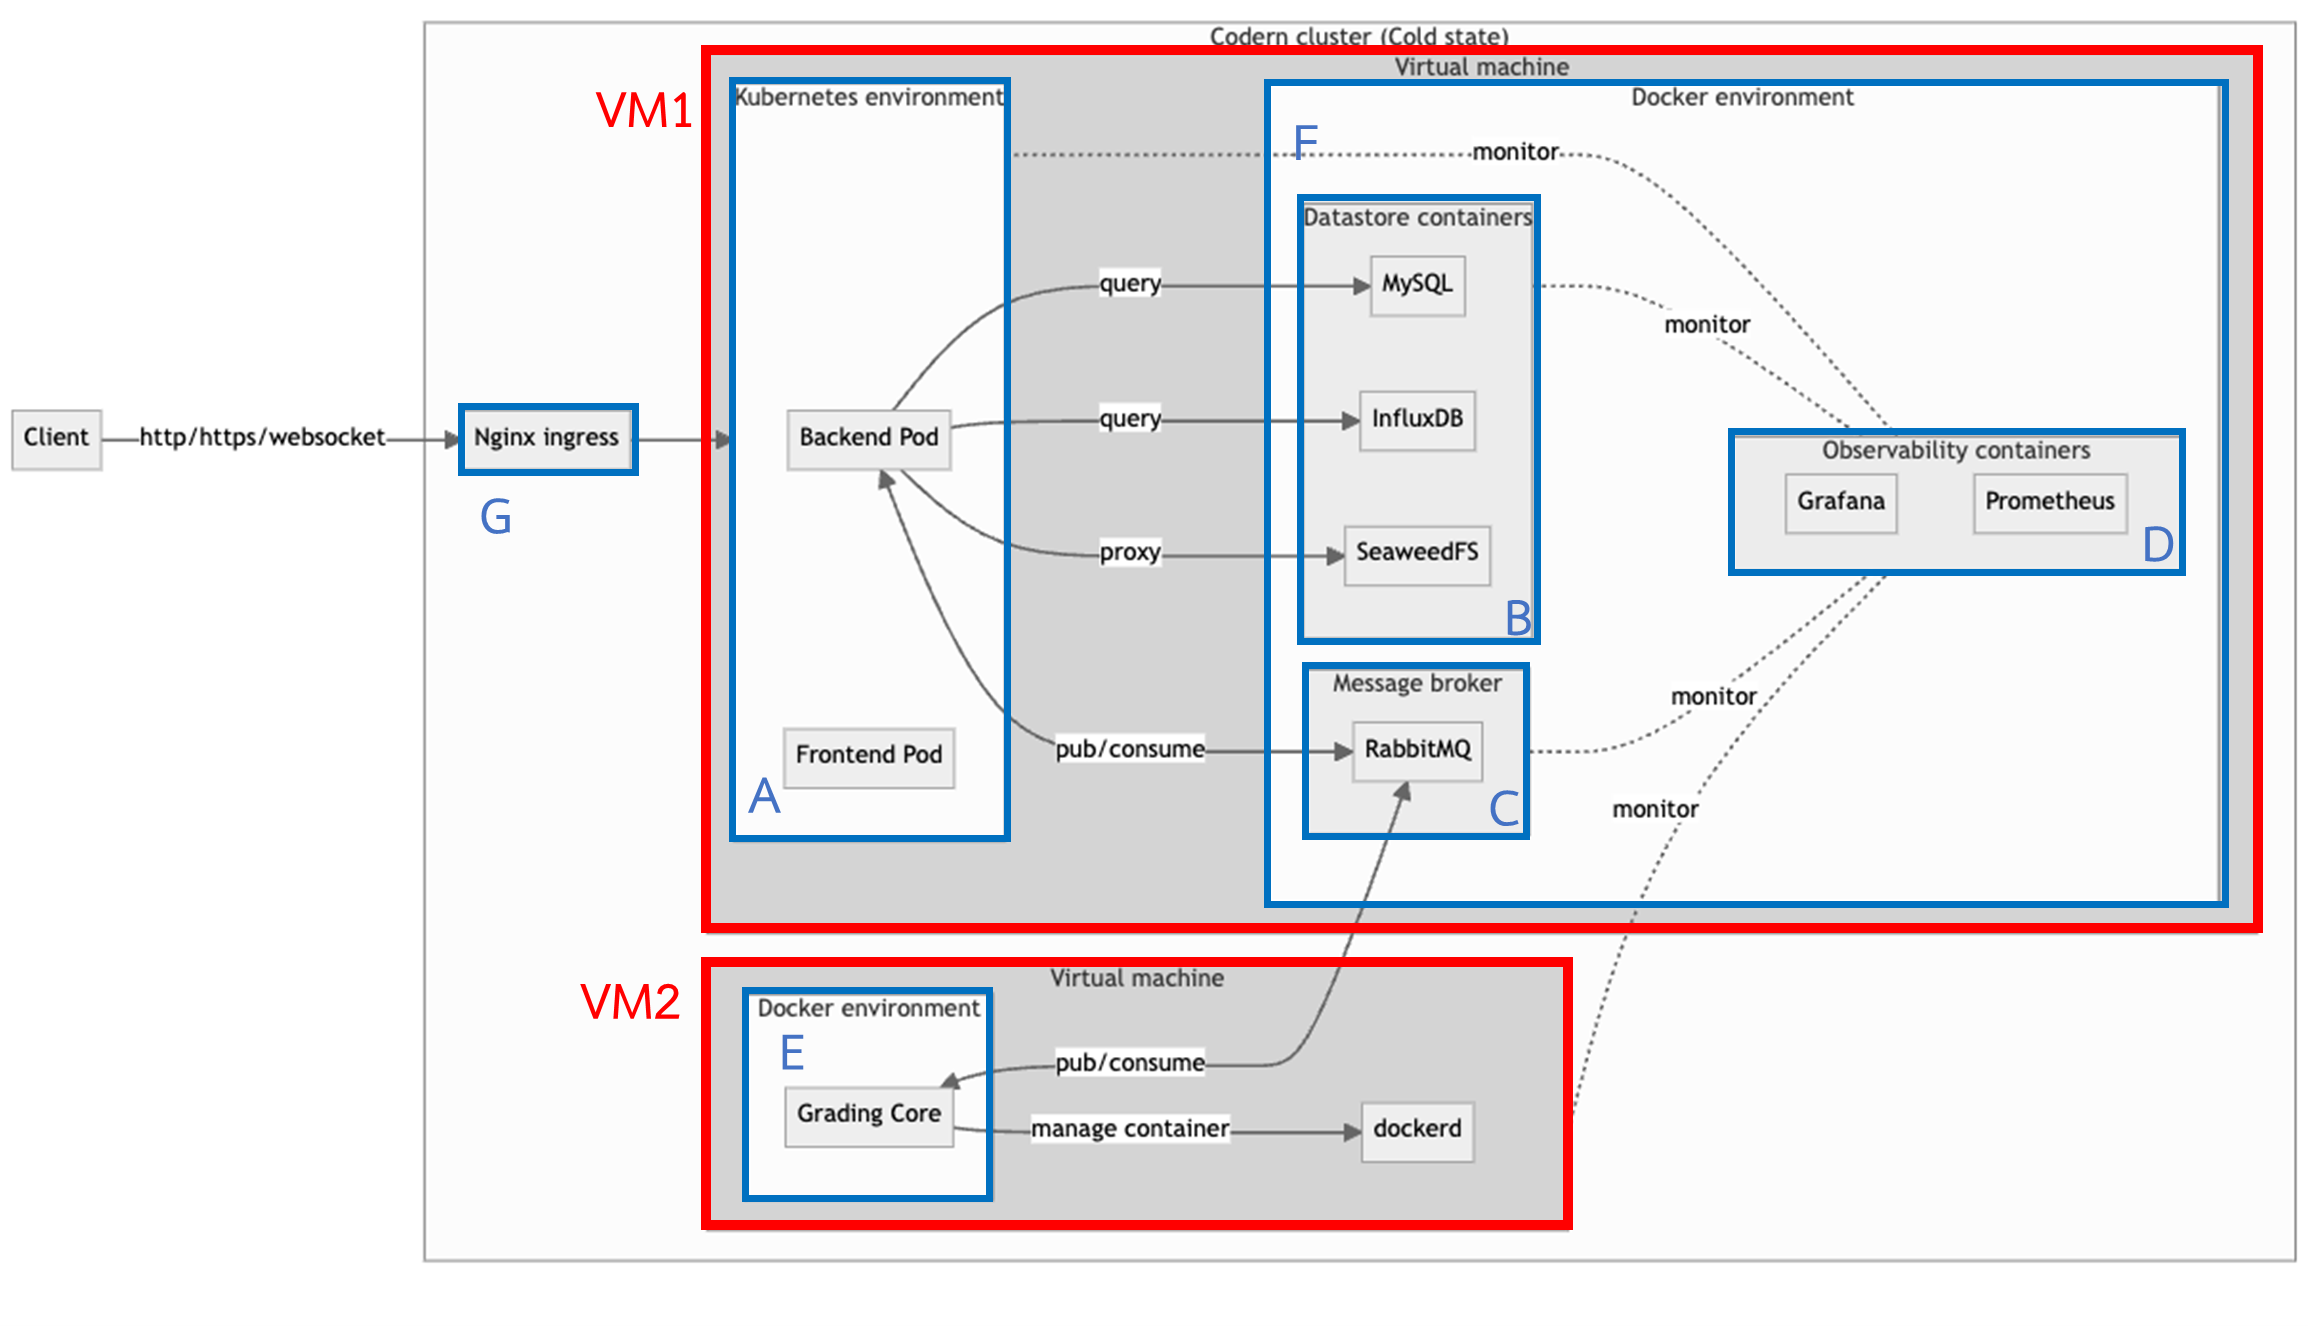
\includegraphics[width=15cm]{figure/diagram/architecture-v1.png}
    % }
    \caption[ภาพเเผนผังสถาปัตยกรรมระบบของซอฟต์เเวร์]{ภาพเเผนผังสถาปัตยกรรมระบบของซอฟต์เเวร์ วาดด้วย \href{https://mermaid.js.org/}{Mermaid JS}}\label{fig:arch}
    \end{figure}
    \begin{flushleft}
    แผนภาพในรูปที่~\ref{fig:arch} แสดงสถาปัตยกรรมระบบแบบกระจาย เครื่องเสมือนสองเครื่อง (เรียกว่า VM1 และ VM2) ภายใน cluster ที่เรียกว่า “Codern Cluster”
    \end{flushleft}
    \begin{flushleft}
    ใน VM1 มีการวางรูปแบบซอฟต์แวร์เป็นรูปแบบ Kubernetes (กรอบ A ในรูป) ที่มี pod ชื่อ backend และ frontend pod โดย pod เหล่านี้จะติดต่อสื่อสารกับส่วนประกอบต่างอื่นๆ ใน container ที่ host โดย Docker ในเครื่องเดียวกัน Docker (กรอบ F ในรูป) ในเครื่อง VM1 จะ host คอนเทนเนอร์ 3 อัน ได้แก่แหล่งเก็บข้อมูลหรือฐานข้อมูลต่าง ๆ (กรอบ B) อาทิเช่น MySQL, InfluxDB และ SeaweedFS, ตัว message broker (กรอบ C) หรือ RabbitMQ ซึ่งก็คือโมดูล ที่เปิดบริการสำหรับการส่งข้อมูลและสื่อสารไปยัง VM2 เพื่อส่งไฟล์โปรแกรมไปตรวจ และสุดท้ายก็คือ monitoring tool อย่าง Grafana และ Prometheus (กรอบ D) ซึ่งเป็นเครื่องมือสำหรับการตรวจดู สอดส่องดูแล วิเคราะห์หาข้อบกพร่อง และวัดประสิทธิภาพการทำงานของแต่ละส่วนของซอฟต์แวร์
    \end{flushleft}
    \begin{flushleft} 
    ใน VM2 ก็มี Docker ที่ host ตัว container อยู่เช่นกัน โดย container นี้จะเปิด Grading Core ไว้ ซึ่งทำหน้าที่เป็นตัวโมดูลโปรแกรมสำหรับตรวจไฟล์โปรแกรมที่ผู้ใช้ได้ส่งเข้ามาจาก VM1 ผ่าน message broker หลังจากตรวจเสร็จก็จะส่งผลตรวจกลับไปยัง message broker
    \end{flushleft}
    \begin{flushleft}
    คำขอของผู้ใช้จะถูกประมวลผลโดยตัวควบคุม Nginx Ingress (กรอบ G ในรูป) เพื่อส่งคำขอของ client ไป Kubernetes cluster ที่ได้ host ไว้ เพื่อประมวลผล
    \end{flushleft}

\pagebreak
\section{ส่วนประสานต่อผู้ใช้}
    \begin{flushleft}
    สำหรับในส่วน UI ทางคณะผู้จัดทำจะนำเสนอหน้าส่วนประสานต่อผู้ใช้ที่ได้ออกแบบไว้ทั้งหมด ดังนี้
    \end{flushleft}
    
    %%%%%%%%%%% LOGIN %%%%%%%%%%%
    \hypertarget{ui-login}{
        \begin{figure}[H]
        \centering
        % \fbox{
            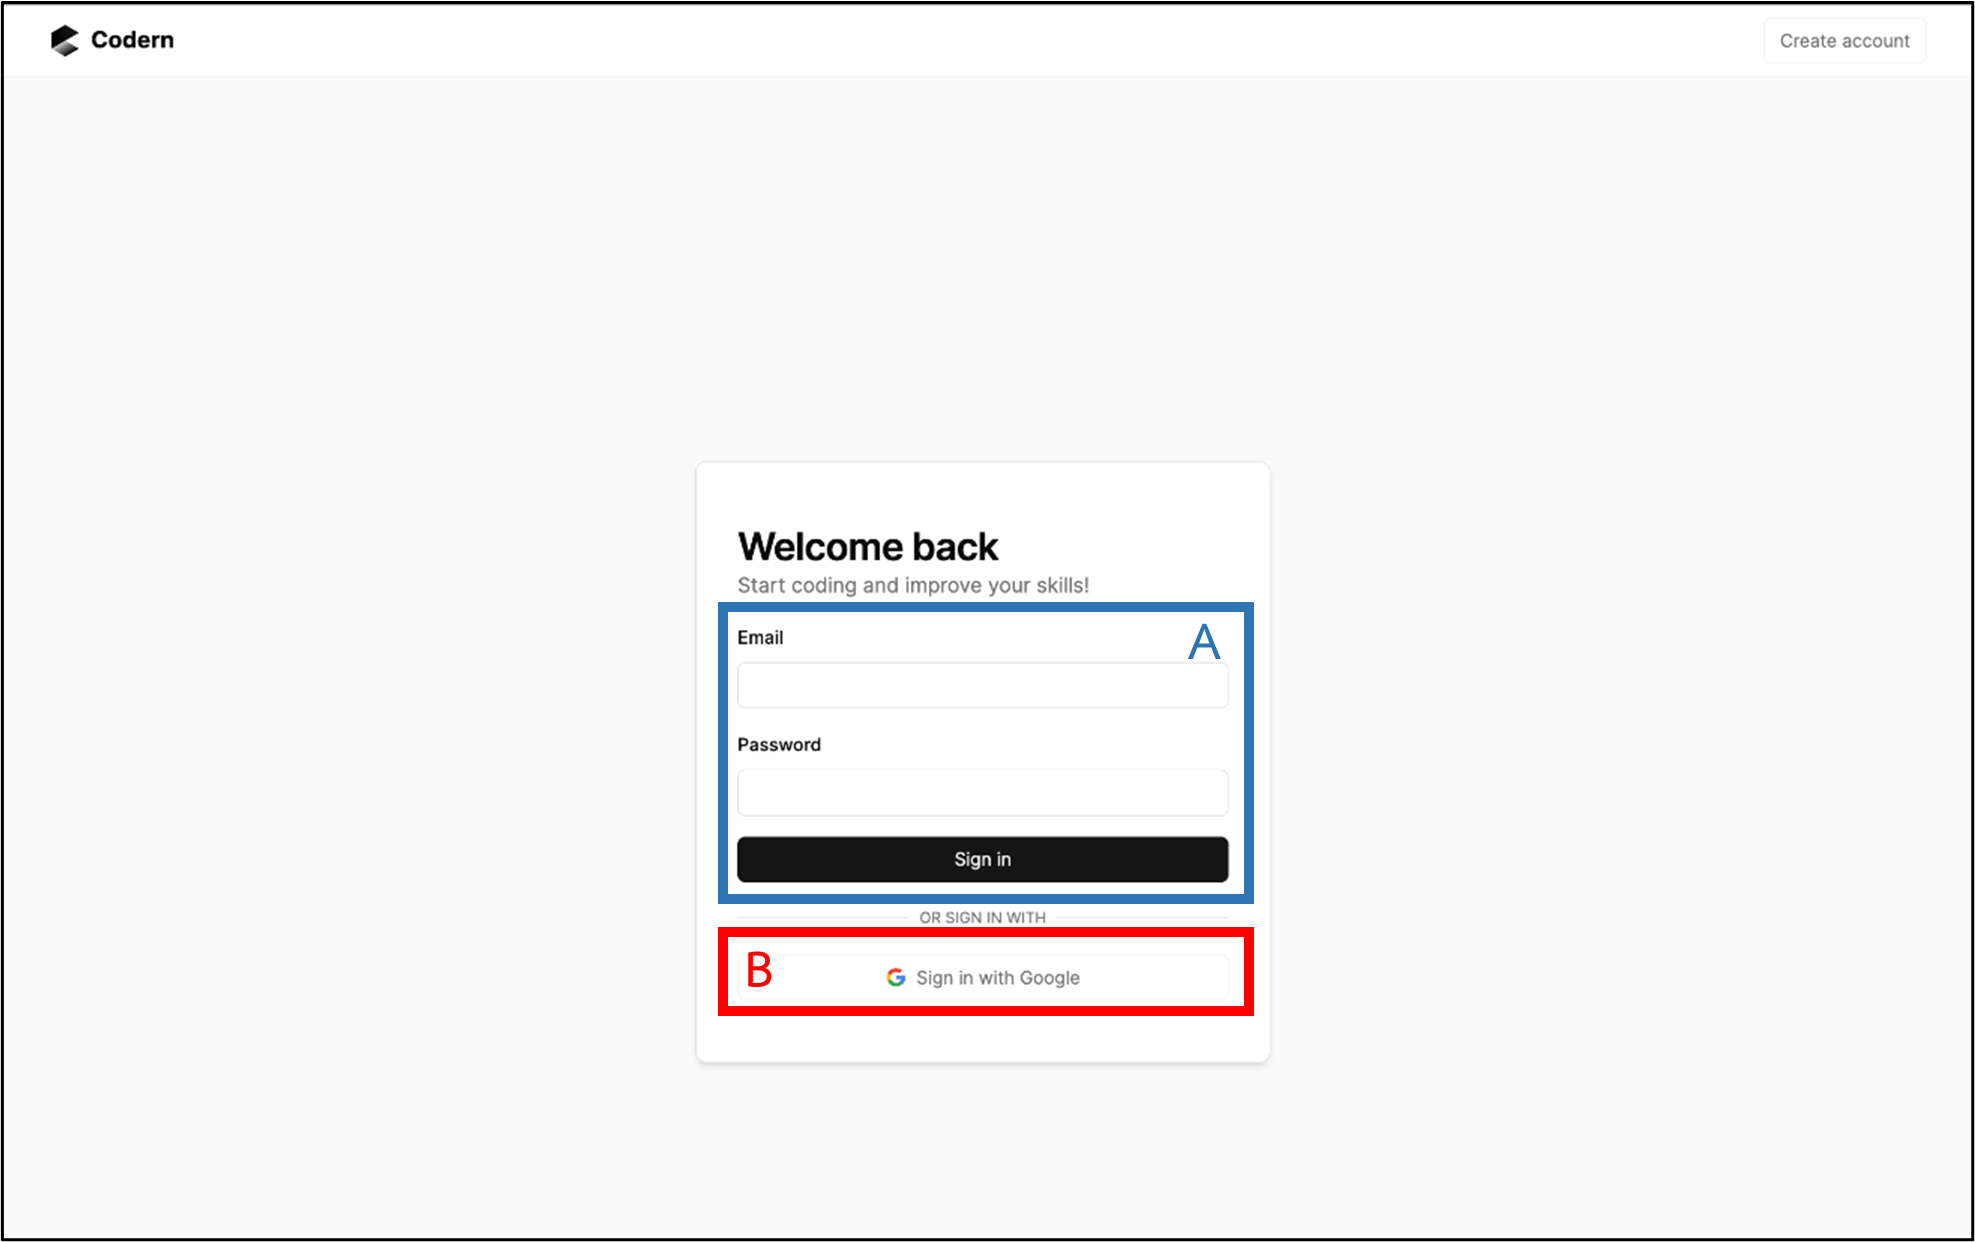
\includegraphics[width=15cm]{figure/ui/ui-login1.png}
        % }
        \caption[ส่วนประสานต่อผู้ใช้ หน้าเข้าสู่ระบบ]{ส่วนประสานต่อผู้ใช้ หน้าเข้าสู่ระบบ}\label{fig:ui-login}
        \end{figure}
    }
    
    \begin{flushleft}
    ในรูปที่~\ref{fig:ui-login} เป็นหน้าสำหรับล็อกอินเข้าระบบใช้งานทั้งหมดของซอฟต์แวร์ โดยสามารถเลือกล็อกอินได้สองวิธี; ด้วยอีเมลเเละรหัสผ่าน (กรอบสีน้ำเงิน A) และล็อกอินผ่านกูเกิ้ล (กรอบสีแดง B) 
    \end{flushleft}

    %%%%%%%%%%% DASHBOARD %%%%%%%%%%%
    \hypertarget{ui-dashboard1}{
        \begin{figure}[H]
        \centering
        % \fbox{
            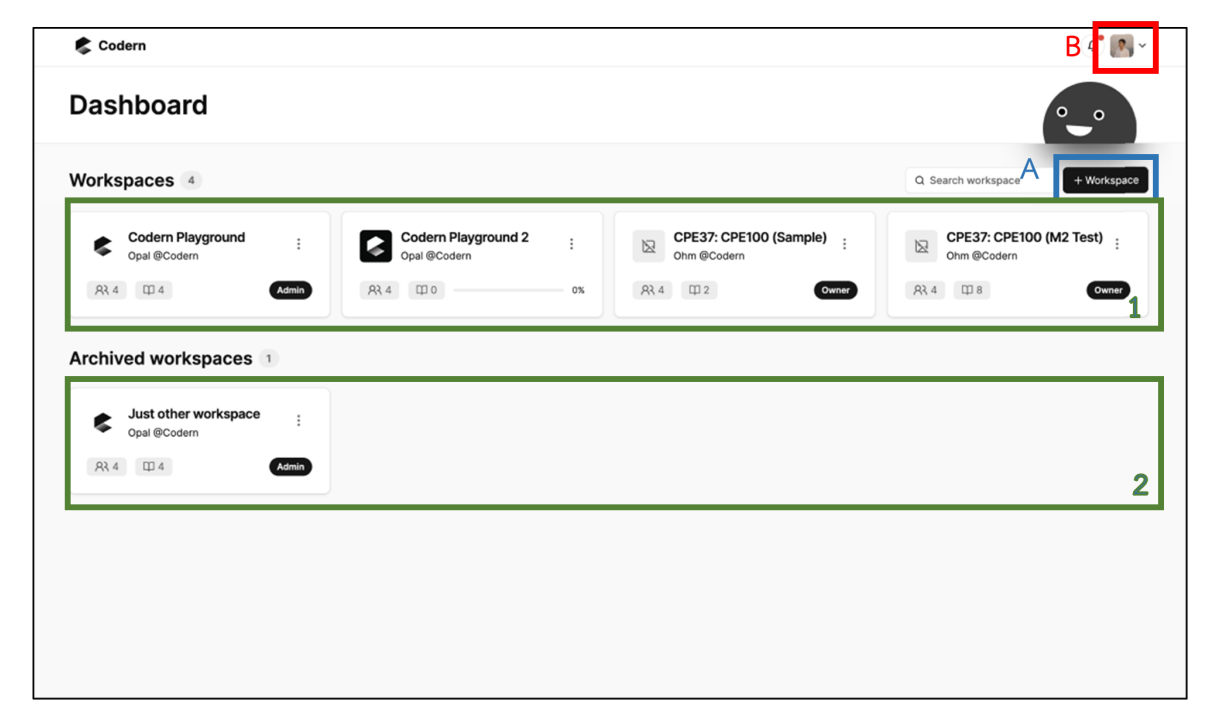
\includegraphics[width=15cm]{figure/ui/ui-dashboard1.png}
        % }
        \caption[ส่วนประสานต่อผู้ใช้ หน้าเเผงควบคุม (1)]{ส่วนประสานต่อผู้ใช้ หน้าเเผงควบคุม}\label{fig:ui-dashboard1}
        \end{figure}
    }

    \begin{flushleft}
    เมื่อเข้าสู่ระบบเรียบร้อยแล้ว จากนั้นจะไปสู่หน้าแสดงรายการห้องทั้งหมดที่ผู้ใช้ได้เข้าร่วม ดังรูปที่~\ref{fig:ui-dashboard1} ส่วนต่อประสานกับผู้ใช้หน้าแสดงรายการห้องที่ผู้ใช้ได้เข้าร่วมอยู่ มีทั้งการแสดงห้องเรียนหรือกลุ่มเรียนทั้งหมดที่เคยเข้าร่วมในส่วน “All Workspaces” (โซนที่ 1) และแสดงห้องเรียนหรือกลุ่มเรียนที่ได้สิ้นสุดคอร์สเรียนหรือสิ้นสุดการใช้งานไปแล้วในส่วน “Archived workspaces” (โซนที่ 2) ผู้ใช้สามารถที่จะกดเข้าร่วมห้องใหม่ได้ที่ปุ่ม “Add Workspace” ตรงมุมขวาบนในกรอบสีน้ำเงิน A และสามารถกดเพื่อแก้ไขข้อมูลเกี่ยวกับบัญชีของตัวเองได้ที่ปุ่มไอคอนอวาตาร์รูปของตนบริเวณมุมขวาบนสุดในกรอบสีแดง B
    \end{flushleft}
    
    \hypertarget{ui-dashboard2}{
        \begin{figure}[H]
        \centering
            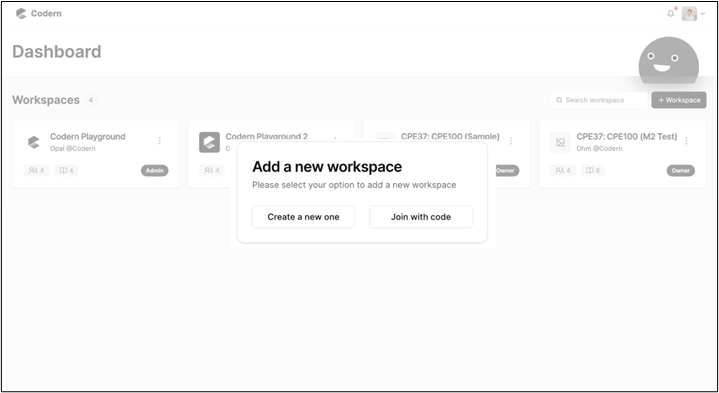
\includegraphics[width=15cm]{figure/ui/ui-dashboard2.png}
            \caption[ส่วนประสานต่อผู้ใช้ หน้าเเผงควบคุม (2)]{ส่วนประสานต่อผู้ใช้ หน้าเเผงควบคุม หลังกดปุ่มเพิ่ม Workspace}\label{fig:ui-dashboard2}
        \end{figure}
    }
    \begin{flushleft}
    โดยเมื่อผู้ใช้กดเข้าร่วมห้องใหม่ที่ปุ่ม “Add Workspace” แล้ว จะปรากฏกล่องข้อความแจ้งเตือนเพื่อแสดงสองทางเลือก ดังภาพที่~\ref{fig:ui-dashboard2} ได้แก่ “Create a new one” ซึ่งผู้ใช้จะสามารถกดเพื่อเข้าสู่หน้าการสร้างห้องเรียนใหม่ โดยกรอกข้อมูลชื่อของห้องเรียน รายละเอียด และรูปภาพ เมื่อกดปุ่ม "Create a new one" แล้ว ห้องเรียนก็จะถูกสร้าง ดังภาพที่~\ref{fig:ui-dashboard3} และ “Join with code” ซึ่งผู้ใช้สามารถกดเพื่อกรอกรหัสเข้าร่วมห้องเรียนที่ได้มีการสร้างไว้ก่อนอยู่แล้วได้ ดังภาพที่~\ref{fig:ui-dashboard4}
    \end{flushleft}


    %%%%%%%%%%% CREATE WORKSPACE %%%%%%%%%%%
    \hypertarget{ui-dashboard3}{
        \begin{figure}[H]
        \centering
            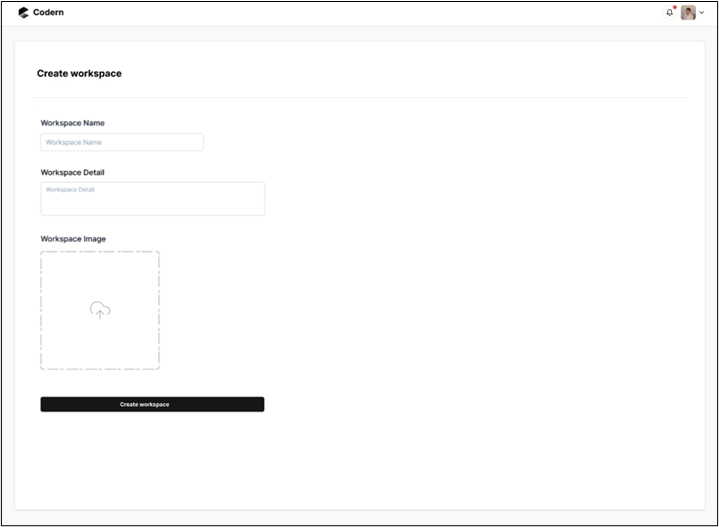
\includegraphics[width=15cm]{figure/ui/ui-dashboard3.png}
            \caption[ส่วนประสานต่อผู้ใช้ หน้าเเผงควบคุม (3)]{ส่วนประสานต่อผู้ใช้ หน้าเเผงควบคุม หลังกดปุ่ม "Create a new one" ในรูปที่~\ref{fig:ui-dashboard2}}
            \label{fig:ui-dashboard3}
        \end{figure}
    }
    
    \hypertarget{ui-dashboard4}{
        \begin{figure}[H]
        \centering
            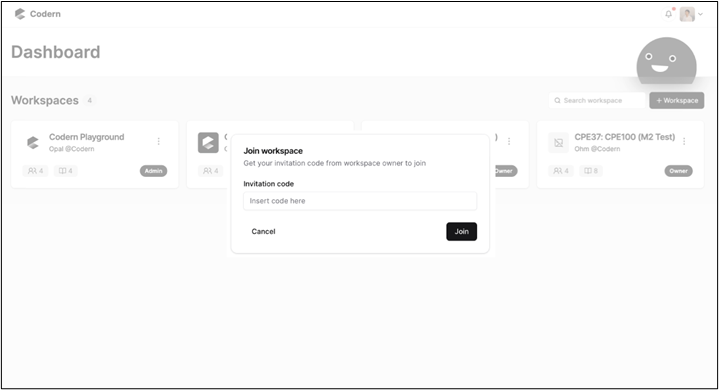
\includegraphics[width=15cm]{figure/ui/ui-dashboard4.png}
            \caption[ส่วนประสานต่อผู้ใช้ หน้าเเผงควบคุม (4)]{ส่วนประสานต่อผู้ใช้ หน้าเเผงควบคุม หลังกดปุ่ม "Join with code" ในรูปที่~\ref{fig:ui-dashboard2}}
            \label{fig:ui-dashboard4}
        \end{figure}
    }

    \hypertarget{ui-dashboard5}{
        \begin{figure}[H]
        \centering
            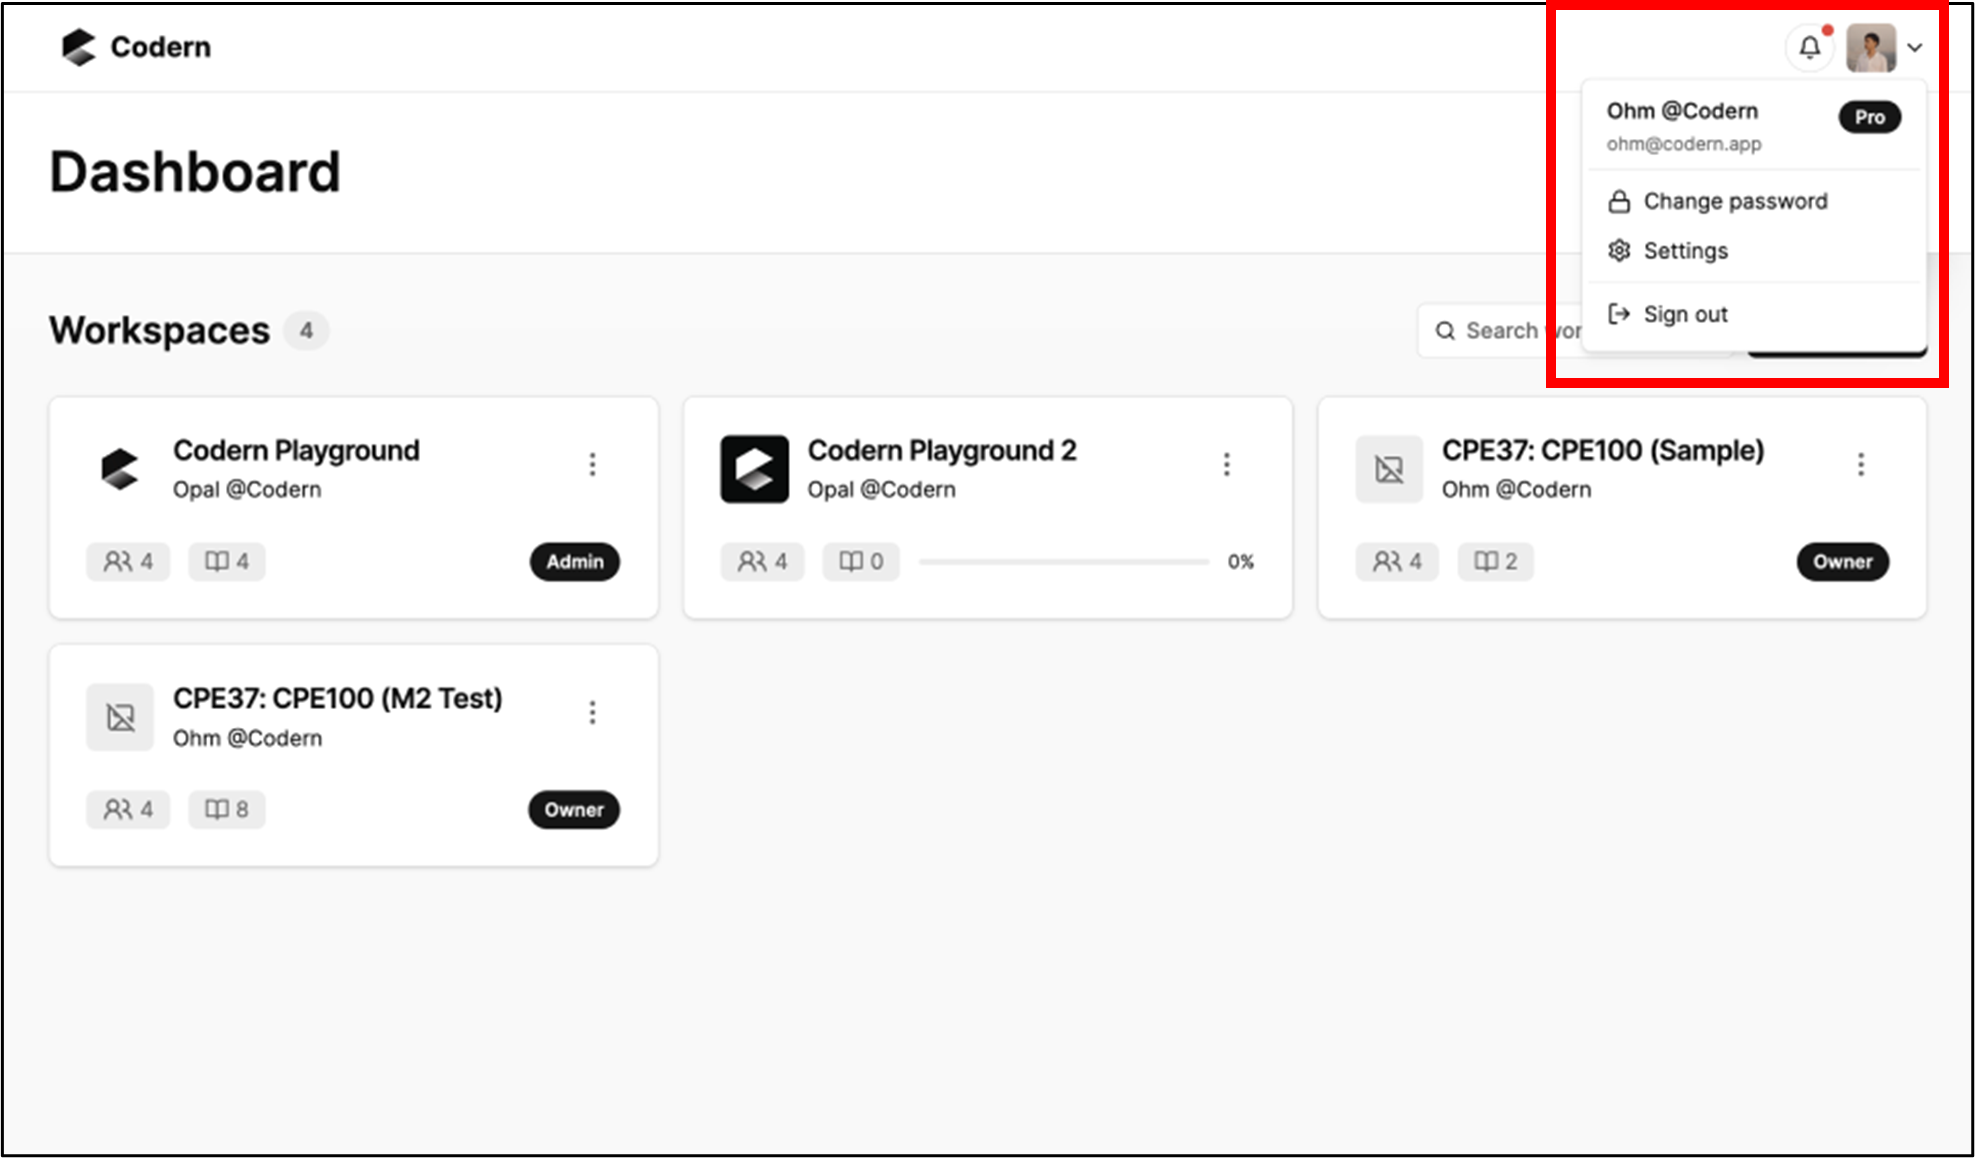
\includegraphics[width=15cm]{figure/ui/ui-dashboard5.png}
            \caption[ส่วนประสานต่อผู้ใช้ หน้าเเผงควบคุม (5)]{ส่วนประสานต่อผู้ใช้ หน้าเเผงควบคุม หากกดรูป Avatar ตรงมุมขวาบน ในรูปที่~\ref{fig:ui-dashboard2}}
            \label{fig:ui-dashboard5}
        \end{figure}
    }
    \begin{flushleft}
    หากกดปุ่มไอคอนอวาตาร์รูปของตนบริเวณมุมขวาบนสุดในกรอบสีแดง B ในภาพที่~\ref{fig:ui-dashboard2} ก็จะปรากฏ Dropdown ลงมาดังภาพที่~\ref{fig:ui-dashboard5} (กรอบสีแดง) ประกอบด้วย 3 เมนู ได้แก่ "Change password", "Settings" และ "Sign out"
    \end{flushleft}

    %%%%%%%%%%% CHANGE PASSWORD %%%%%%%%%%%
    \hypertarget{ui-settings-password}{
        \begin{figure}[H]
        \centering
            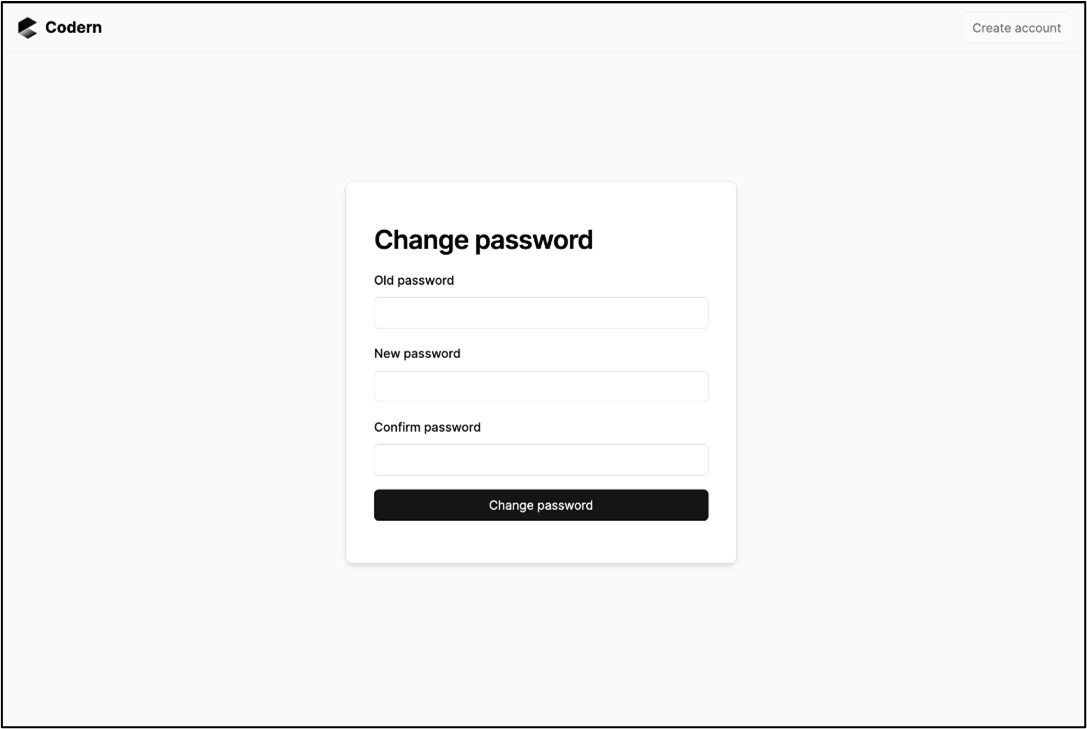
\includegraphics[width=15cm]{figure/ui/ui-settings-password.png}
            \caption[ส่วนประสานต่อผู้ใช้ หน้าเเผงควบคุม (6)]{ส่วนประสานต่อผู้ใช้ หน้าเเผงควบคุม หากกดปุ่ม "Change Password" ในรูปที่~\ref{fig:ui-dashboard5}{3.8}}
            \label{fig:ui-settings-password}
        \end{figure}
    }
    \begin{flushleft}
    เมื่อกดปุ่ม "Change password" ในรูปที่~\ref{fig:ui-dashboard5} จะนำไปสู่หน้าเปลี่ยนรหัสผ่านเข้าบัญชี ดังภาพที่~\ref{fig:ui-settings-password} โดยจะเปลี่ยนรหัสผ่านบัญชีได้โดยการกรอกรหัสผ่านเก่าให้ถูกต้อง จากนั้นก็กรอกรหัสผ่านใหม่ที่ต้องการ และทำการยืนยันรหัสผ่านใหม่ซ้ำอีกครั้ง เมื่อกรอกรหัสทั้งหมดถูกต้อง เพียงกดปุ่ม "Change password" ก็จะสามารถเปลี่ยนรหัสผ่านบัญชีใหม่ได้
    \end{flushleft}

    \begin{flushleft}
    ถ้ากดปุ่ม Settings ในรูปที่~\ref{fig:ui-dashboard5} จะนำไปสู่หน้าแก้ไขข้อมูลส่วนตัวของเจ้าของบัญชี ได้แก่ ชื่อบัญชี และรูปภาพอวาตาร์ ดังภาพที่~\ref{fig:ui-settings}
    \end{flushleft}

    %%%%%%%%%%% SETTINGS %%%%%%%%%%%
    \hypertarget{ui-settings}{
        \begin{figure}[H]
        \centering
            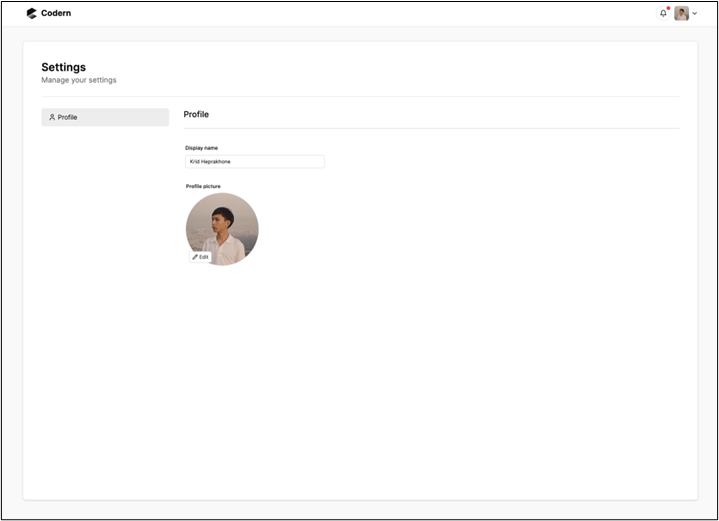
\includegraphics[width=15cm]{figure/ui/ui-settings.png}
            \caption[ส่วนประสานต่อผู้ใช้ หน้าตั้งค่าของผู้ใช้]{ส่วนประสานต่อผู้ใช้ หน้าตั้งค่าของผู้ใช้ หากกดปุ่ม "Settings" ในรูปที่ \hyperlink{ui-dashboard5}{3.8}}
            \label{fig:ui-settings}
        \end{figure}
    }
    \begin{flushleft}
    แต่ถ้ากดปุ่ม Sign out ในรูปที่~\ref{fig:ui-dashboard5} จะกลับไปสู่หน้าล็อกอินแรกสุดของระบบ ดังภาพที่~\ref{fig:ui-login}
    \end{flushleft}
    \pagebreak
    
    \begin{flushleft}
    หากเป็นผู้ดูแล ในการแสดงรายการห้องทั้งหมด จะเปลี่ยนเป็นมุมมองของผู้ดูแลระบบดังรูปที่~\ref{fig:ui-org-dashboard1} แผงควบคุมดังกล่าว มีบทบาทและการจัดวางที่คล้ายคลึงกันกับฝั่งของผู้ใช้ทั่วไปในรูปที่~\ref{fig:ui-dashboard1} ต่างกันที่การจัดหมวดหมู่ห้องเรียน ทั้งนี้ก็จะมีปุ่มกดที่มุมขวาบนเป็นปุ่มที่สำคัญที่สุดก็คือ “Create Workspace” ที่เป็นปุ่มในการสร้างห้องเรียนหรือกลุ่มเรียนใหม่ (กรอบสีแดง A ในรูป~\ref{fig:ui-org-dashboard1}) ซึ่งหากกดต่อไป ก็จะไปสู่หน้าสร้างห้องเรียนหรือกลุ่มเรียนใหม่เหมือนกับในรูปที่~\ref{fig:ui-dashboard3}
    \end{flushleft}

    %%%%%%%%%%% ORGANIZER DASHBOARD %%%%%%%%%%%
    \hypertarget{ui-org-dashboard1}{
        \begin{figure}[H]
        \centering
            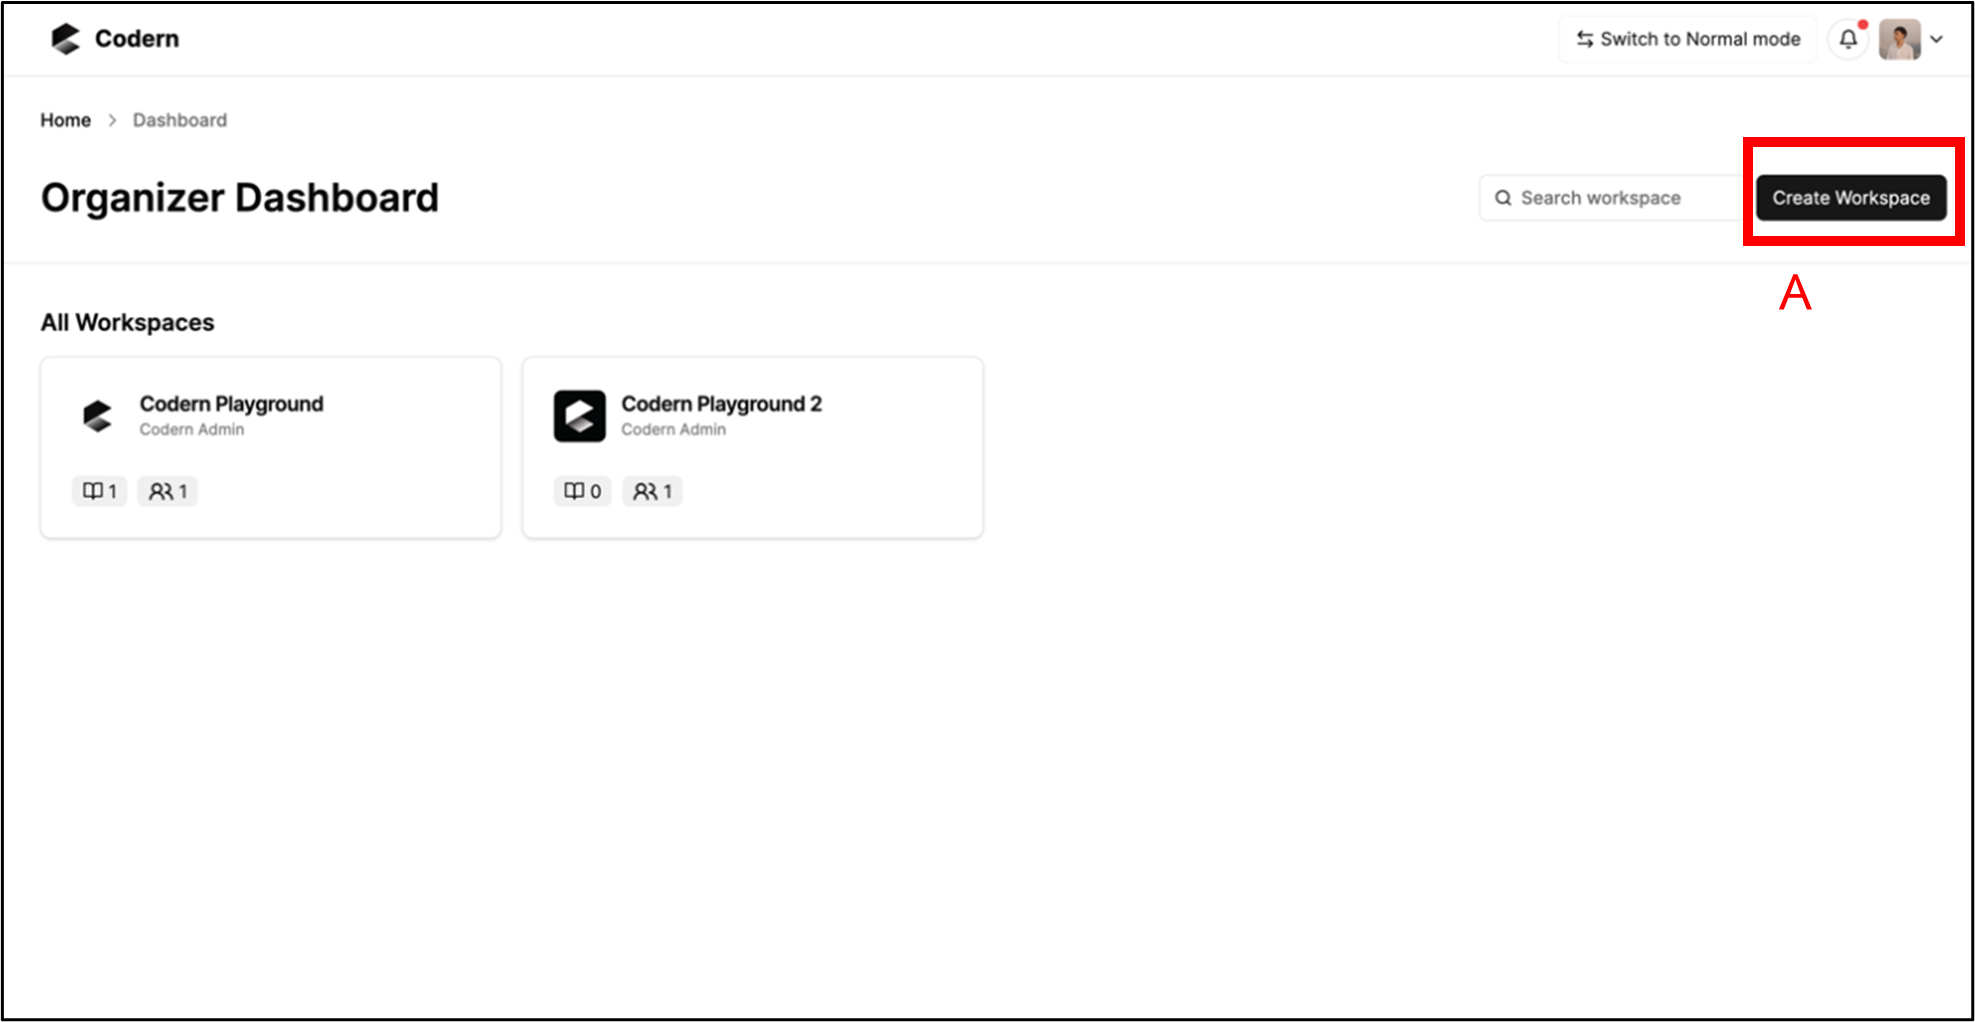
\includegraphics[width=15cm]{figure/ui/ui-org-dashboard1.png}
            \caption[ส่วนประสานต่อผู้ใช้ หน้าเเผงควบคุมของผู้ดูเเลระบบ]{ส่วนประสานต่อผู้ใช้ หน้าเเผงควบคุมในมุมมองของผู้ดูเเลระบบ}
            \label{fig:ui-org-dashboard1}
        \end{figure}
    }
    \begin{flushleft}
    ถ้าหากกดเข้าห้องเรียนหรือกลุ่มเรียนใด ๆ ในหน้าก่อน (ในรูปที่~\ref{fig:ui-dashboard1}) ก็จะนำมาสู่หน้าจอ ดังรูปที่~\ref{fig:ui-assign1} (หรือรูปที่~\ref{fig:ui-org-assign1} ถ้าหากเป็นแอดมินหรือผู้ดูแล) โดยในหน้านี้ ที่โซนที่ 1 จะแสดงโจทย์ปัญหา การบ้านหรือข้อสอบทั้งหมดที่เจ้าของห้อง/อาจารย์ผู้สอนได้สร้างไว้ แต่ละรายการก็จะแสดงข้อมูลตั้งแต่ชื่องาน, รายละเอียดงาน, ระดับความยาก, จนไปถึงสถานะ นอกจากแสดงโจทย์แล้ว ในส่วนบน ตรงโซนที่ 2 ยังมีการแสดงข้อมูลของห้องเรียนหรือกลุ่มเรียนด้วย ตั้งแต่ชื่อเจ้าของห้อง จำนวนงานในกลุ่มหรือห้อง จำนวนงานที่ผู้ใช้ยังทำไม่เสร็จ จำนวนสมาชิกที่ได้เข้าร่วมห้องหรือกลุ่มนี้
    \end{flushleft}

    %%%%%%%%%%% ASSIGNMENT LIST %%%%%%%%%%%
    % FIX NOTE: No due date is present
    \hypertarget{ui-assign1}{
        \begin{figure}[H]
        \centering
            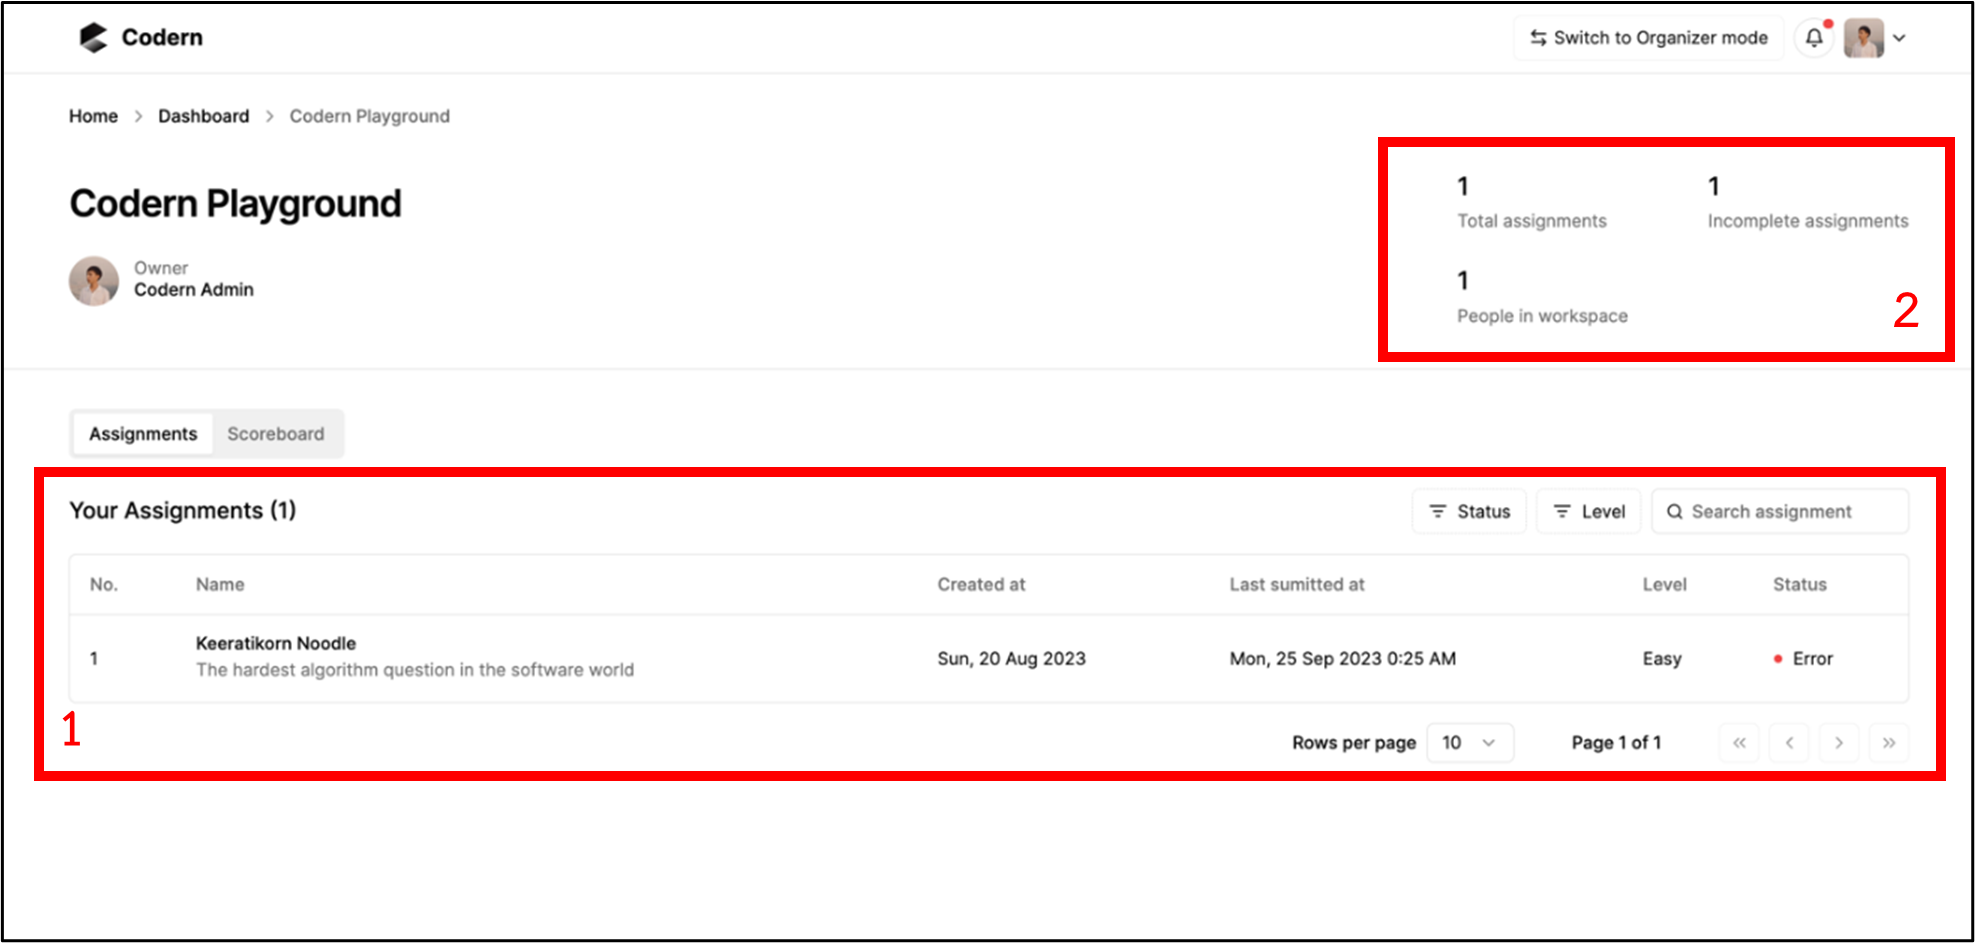
\includegraphics[width=15cm]{figure/ui/ui-assign1.png}
            \caption[ส่วนประสานต่อผู้ใช้ หน้ารายการโจทย์ปัญหา]{ส่วนประสานต่อผู้ใช้ หน้ารายการโจทย์ปัญหา}
            \label{fig:ui-assign1}
        \end{figure}
    }
    
    %%%%%%%%%%% ORGANIZER ASSIGNMENT LIST %%%%%%%%%%%
    \hypertarget{ui-org-assign1}{
        \begin{figure}[H]
        \centering
            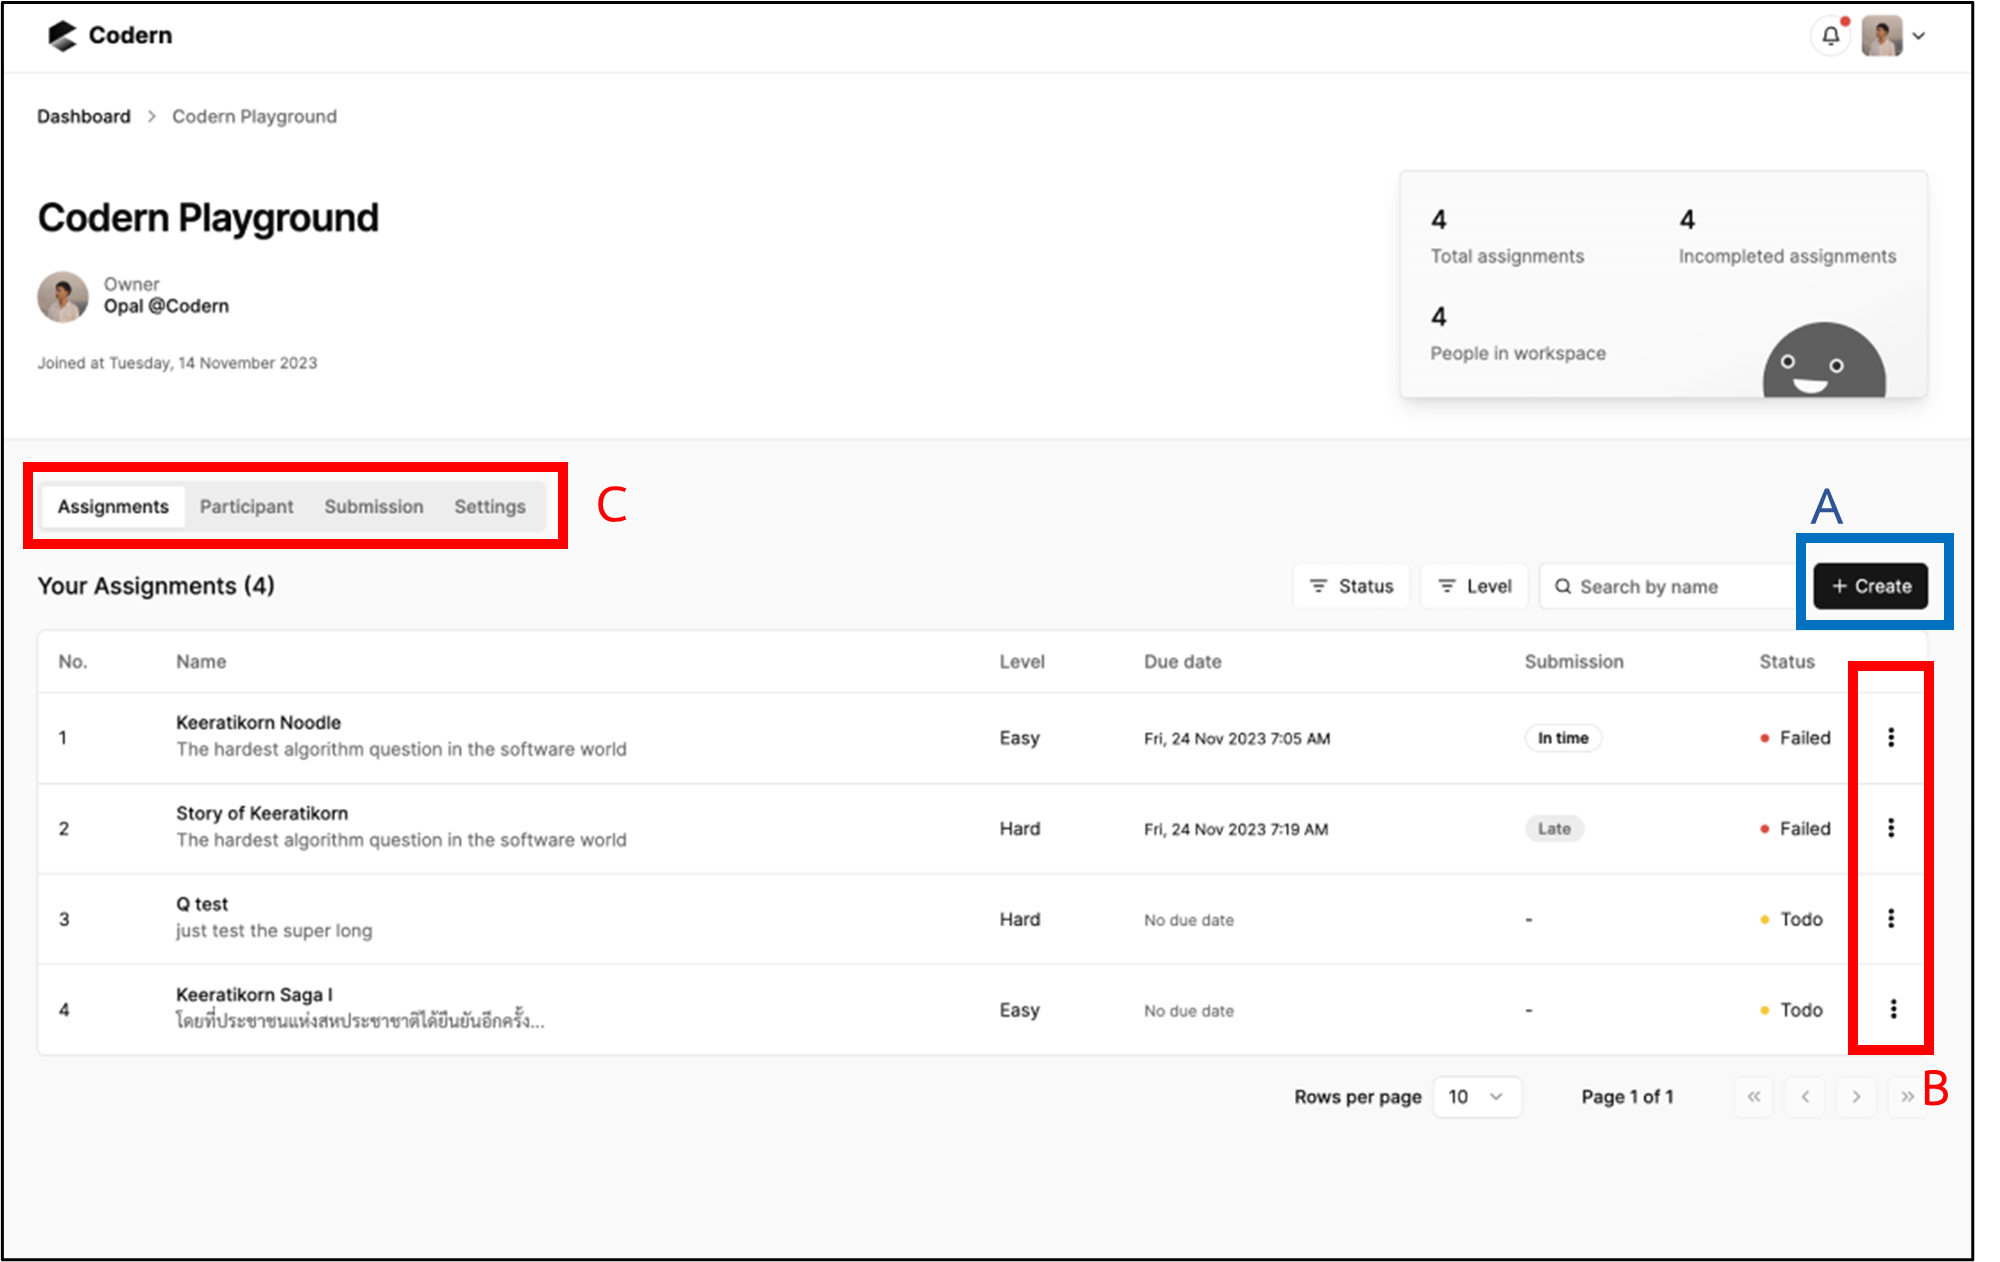
\includegraphics[width=15cm]{figure/ui/ui-assign2.png}
            \caption[ส่วนประสานต่อผู้ใช้ หน้ารายการโจทย์ปัญหาของผู้ดูเเลระบบ]{ส่วนประสานต่อผู้ใช้ หน้ารายการโจทย์ปัญหา ในมุมมองของผู้ดูเเลระบบ}
            \label{fig:ui-org-assign1}
        \end{figure}
    }

    \begin{flushleft}
    ในอีกฝั่ง ในส่วนของผู้ดูแลในรูปที่~\ref{fig:ui-org-assign1} ก็จะแสดงผลคล้ายคลึงกับฝั่งของผู้ใช้ในรูปที่~\ref{fig:ui-assign1} มีความต่างที่มีปุ่ม “Create Assignment” (กรอบสีน้ำเงิน A) ซึ่งเมื่อกดแล้วจะนำไปสู่รูปที่~\ref{fig:ui-org-assign2} ซึ่งเป็นฟอร์มสำหรับสร้างการบ้าน โจทย์ปัญหาหรือข้อสอบ สำหรับให้อาจารย์ผู้สอนหรือเจ้าของห้องได้ใช้, ปุ่มรูป "Kebab Menu" ท้ายสุดของแต่ละแถวเพิ่มขึ้นมา (กรอบสีแดง B) ซึ่งเมื่อกดแล้วจะนำพาไปหน้าเเก้ไขโจทย์ปัญหาข้อนั้นๆ ในหน้านั้น (รูปที่~\ref{fig:ui-org-assign3}) ผู้ดูเเลระบบหรือเจ้าของห้องสามารถแก้ไขข้อมูลของ Assignment นั้น ๆ ได้ 
    \end{flushleft}
    
    \begin{flushleft}
    % Submission tab
    สามารถใช้แถบปุ่ม Tab (ในกรอบ C) สามารถที่จะย้ายหน้า ไปยังเเถบอื่นได้ เเถบดังกล่าวประกอบด้วยหน้า Participants ดังรูปที่~\ref{fig:ui-org-assign4}, Submission ดังรูปที่~\ref{fig:ui-org-assign5}, Settings ดังรูปที่~\ref{fig:ui-org-assign-settings1} \ref{fig:ui-org-assign-settings2} \ref{fig:ui-org-assign-settings3}
    \end{flushleft}

    \pagebreak

    %%%%%%%%%%% ORGANIZER CREATE ASSIGNMENT %%%%%%%%%%%
    \hypertarget{ui-org-assign2}{
        \begin{figure}[H]
        \centering
            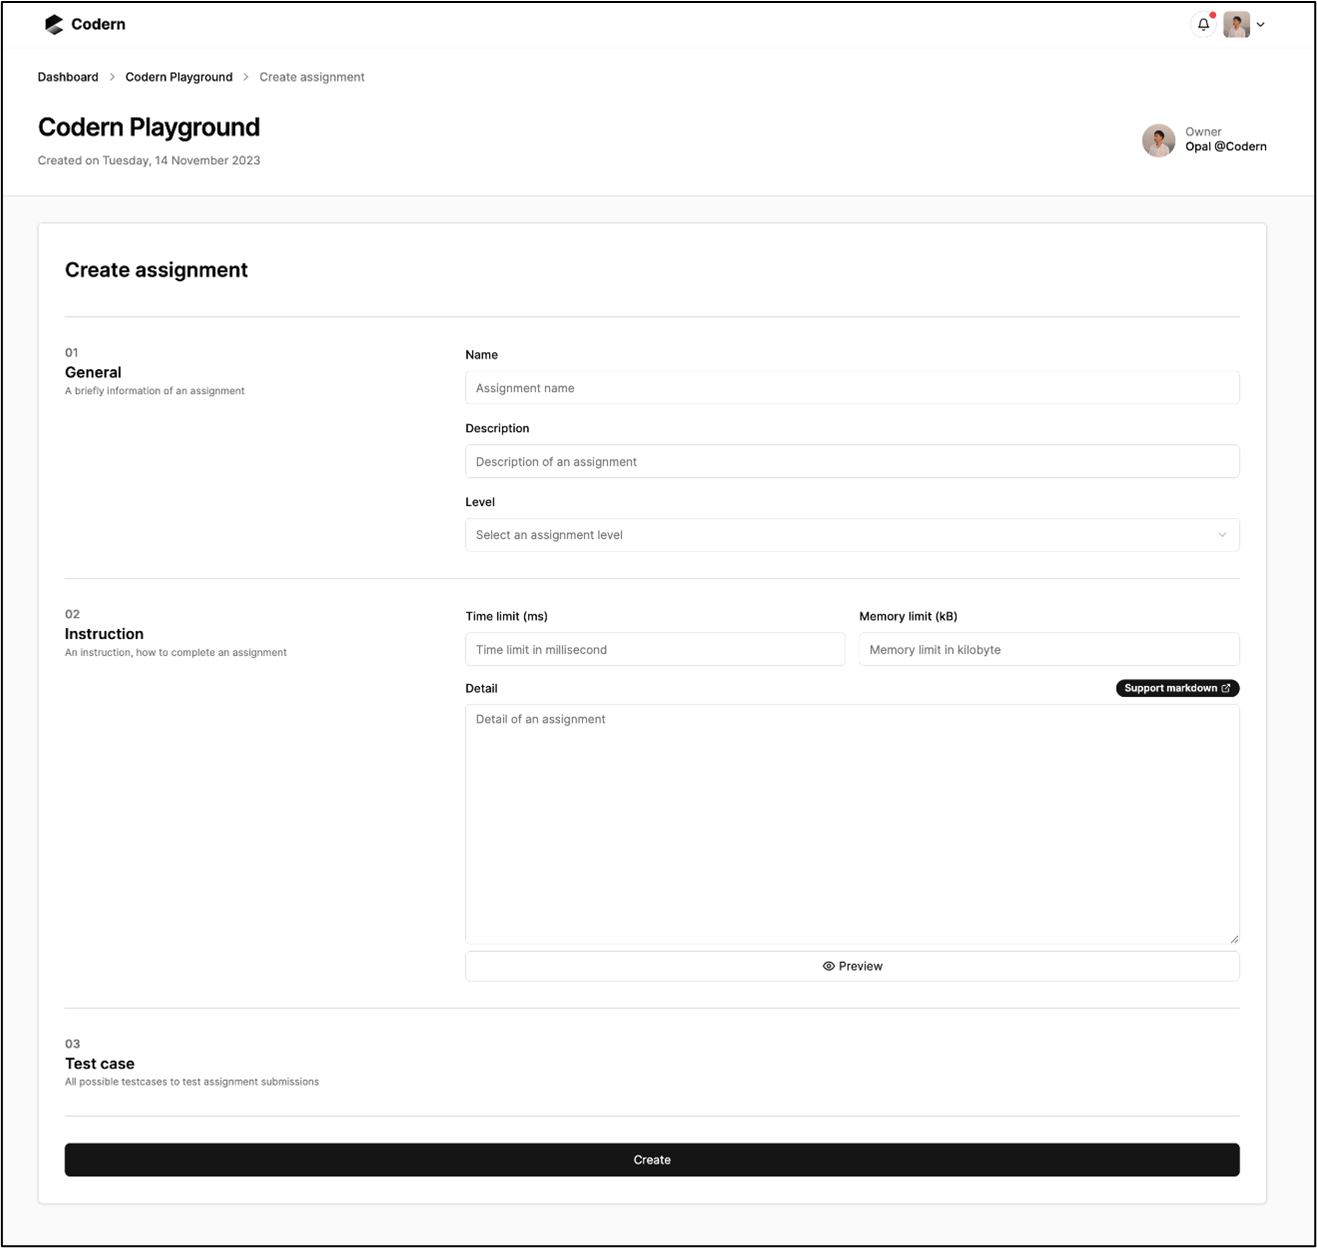
\includegraphics[width=15cm]{figure/ui/ui-assign3.png}
            \caption[ส่วนประสานต่อผู้ใช้ หน้าฟอร์มสร้างโจทย์ปัญหา]{ส่วนประสานต่อผู้ใช้ หน้าฟอร์มสร้างโจทย์ปัญหาของผู้ดูเเลระบบ}
            \label{fig:ui-org-assign2}
        \end{figure}
    }
     %%%%%%%%%%% ORGANIZER EDIT ASSIGNMENT %%%%%%%%%%%
    \hypertarget{ui-org-assign3}{
        \begin{figure}[H]
        \centering
            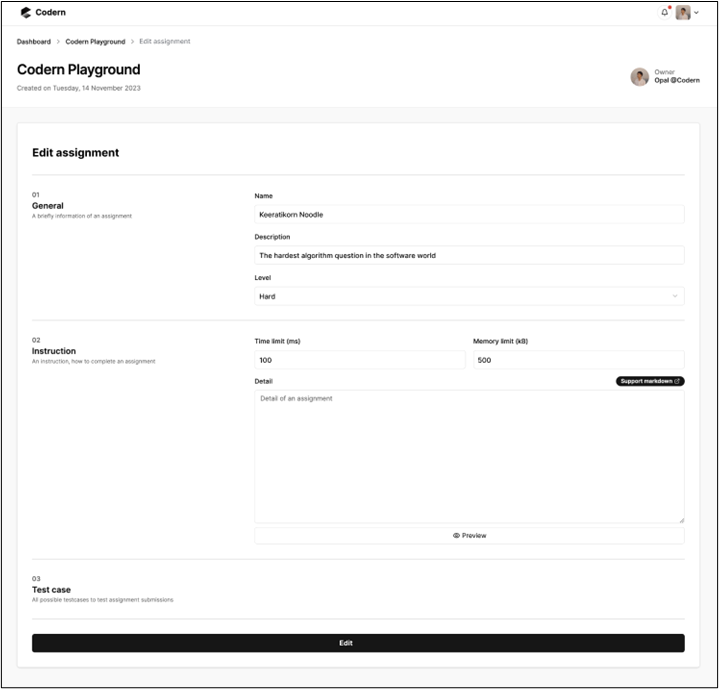
\includegraphics[width=15cm]{figure/ui/ui-assign4.png}
            \caption[ส่วนประสานต่อผู้ใช้ หน้าฟอร์มแก้ไขโจทย์ปัญหา]{ส่วนประสานต่อผู้ใช้ หน้าฟอร์มเเก้ไขโจทย์ปัญหาของผู้ดูเเลระบบ}
            \label{fig:ui-org-assign3}
        \end{figure}
    }
    
    \begin{flushleft}
    ซึ่งภายในรูปที่~\ref{fig:ui-org-assign2} นั้น อาจารย์หรือผู้ดูแลสามารถเพิ่มโจทย์ปัญหาใหม่เข้าสู่ระบบได้ โดยจะมีข้อมูลของโจทย์ปัญหาให้กรอกตามกำหนด ประกอบไปด้วย ชื่องาน, รายละเอียดงาน, ระดับความยาก, จำนวนหน่วยความจำที่ใช้ได้ (Memory Limit), ระยะเวลาที่ใช้ในการหาคำตอบ (Runtime Limit), รายละเอียดของโจทย์, ตัวอย่างผลลัพธ์ (Test case) และนอกจากนี้ยังสามารถกด Preview เพื่อดูตัวอย่างของโจทย์ที่จะออกมาได้อีกด้วย เมื่อกดปุ่ม "Create" ด้านล่างสุด โจทย์ปัญหาก็จะถูกสร้างขึ้น
    \end{flushleft}
    \begin{flushleft}
    ส่วนภายในหน้า Edit Assignment ดังภาพที่~\ref{fig:ui-org-assign3} นั้น จะเป็นหน้าที่อาจารย์หรือผู้ดูแลสามารถแก้ไขข้อมูลของโจทย์ปัญหานั้นๆ ที่ถูกสร้างไว้แล้วได้ โดยจะสามารถแก้ไขข้อมูลได้ทั้งหมด ตั้งแต่ ชื่องาน, รายละเอียดงาน, ระดับความยาก, จำนวนหน่วยความจำที่ใช้ได้ (Memory Limit), ระยะเวลาที่ใช้ในการหาคำตอบ (Runtime Limit), รายละเอียดของโจทย์ และตัวอย่างผลลัพธ์ (Test case)
    \end{flushleft}

    %%%%%%%%%%% ORGANIZER MANAGE USER PARTICIPANTS %%%%%%%%%%%
    \hypertarget{ui-org-assign4}{
        \begin{figure}[H]
        \centering
            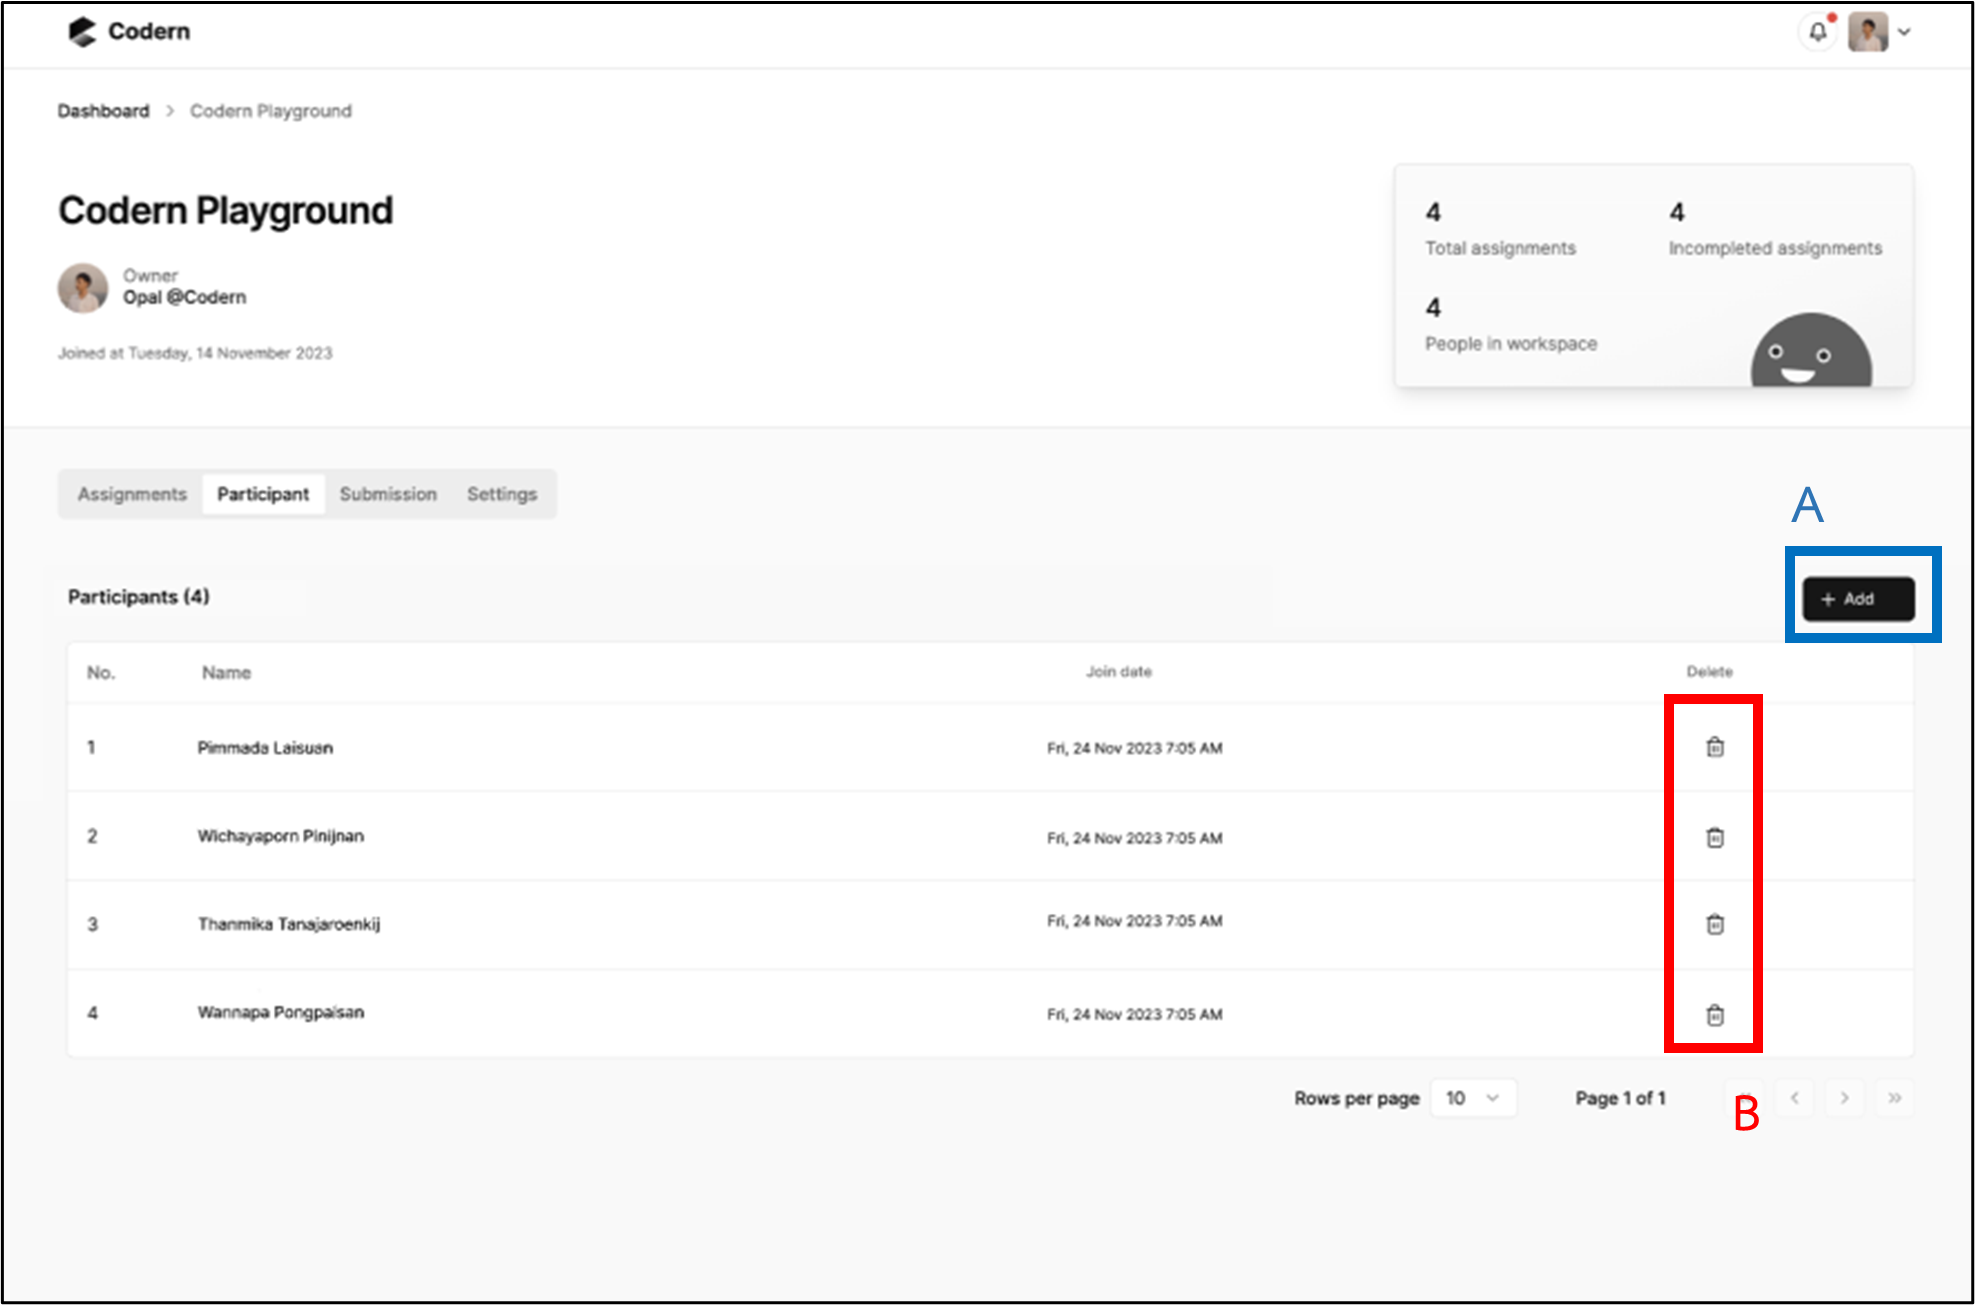
\includegraphics[width=15cm]{figure/ui/ui-assign6.png}
            \caption[ส่วนประสานต่อผู้ใช้ หน้ารายชื่อผู้ใช้ใน Workspace ของผู้ดูเเลระบบ]{ส่วนประสานต่อผู้ใช้ หน้ารายชื่อผู้ใช้ใน Workspace ทั้งหมด ในมุมมองของผู้ดูเเลระบบ}
            \label{fig:ui-org-assign4}
        \end{figure}
    }
    \begin{flushleft}
    หากกดตรง Tab ตรง "Participant" (ตรงกรอบ C รูปที่~\ref{fig:ui-org-assign1}) หน้าในรูปที่~\ref{fig:ui-org-assign4} จะแสดงขึ้นมา โดยหน้าดังกล่าวเป็นหน้าแสดงรายละเอียดสมาชิกของห้องเรียนนั้น ๆ โดยจะแสดงจำนวนสมาชิก รายชื่อนามสกุล วันที่สมาชิกคนนั้น ๆ เข้าร่วมห้องเรียน และผู้ดูเเลระบบจะสามารถลบสมาชิกคนนั้น ๆ ออกจากห้องเรียนได้ด้วยปุ่ม "Delete" ที่ท้ายรายชื่อคนนั้น ๆ (กรอบสีน้ำเงิน A) รวมถึงสามารถเพิ่มสมาชิกใหม่เข้ามาได้ด้วยปุ่ม Add (กรอบสีแดง B) เเต่ถ้าหากเป็นผู้ใช้ธรรมดาทั่วไป จะมองไม่เห็นปุ่ม "Add" หรือปุ่ม "Delete"
    \end{flushleft}
    \pagebreak


    %%%%%%%%%%% ORGANIZER MANAGE SUBMISSION %%%%%%%%%%%
    \begin{figure}[H]
    \centering
        \fbox{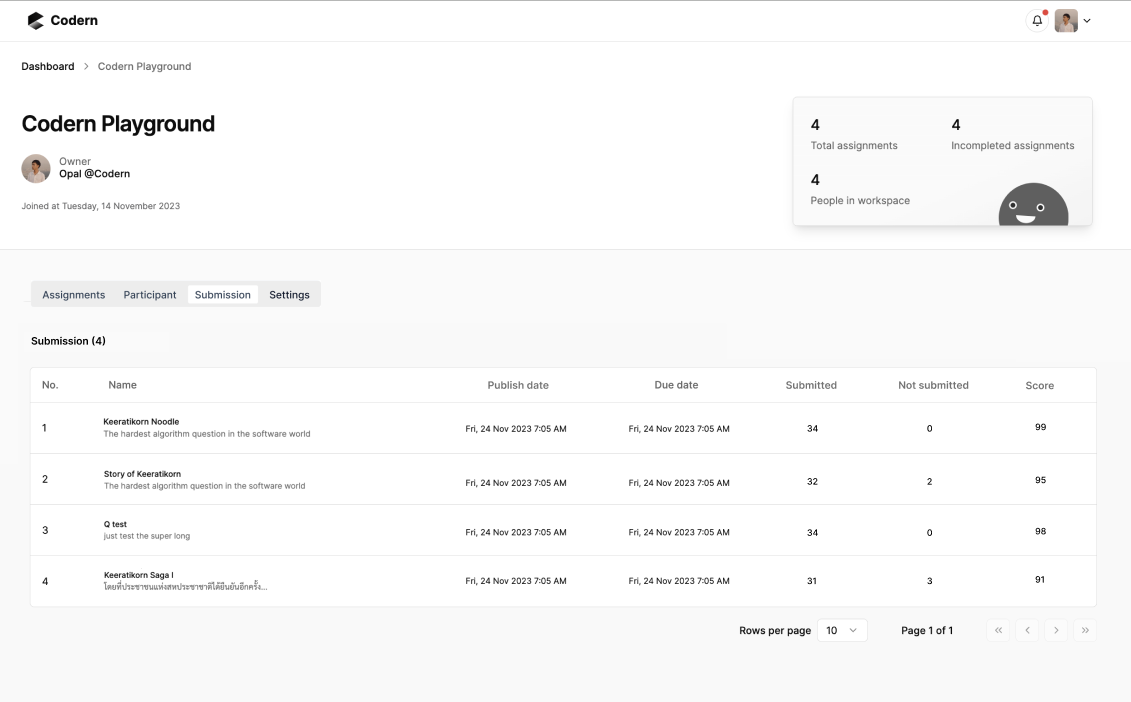
\includegraphics[width=15cm]{figure/ui/ui-assign7.png}}
        \caption[ส่วนประสานต่อผู้ใช้ หน้ารายการโปรแกรมที่ส่งเข้ามาใน Workspace ของผู้ดูเเลระบบ]{ส่วนประสานต่อผู้ใช้ หน้ารายการโปรแกรมที่ผู้ใช้ส่งเข้ามาใน Workspace ในมุมมองของผู้ดูเเลระบบ}
        \label{fig:ui-org-assign5}
    \end{figure}
    \begin{flushleft}
    ต่อมา เมื่อกดปุ่ม Tab ที่ "Submission" แล้ว จะปรากฏหน้าดังรูปที่ ~\ref{fig:ui-org-assign5} โดยหน้าดังกล่าวเป็นหน้าแสดงรายละเอียดรายการโปรแกรมทั้งหมดที่มีของห้องเรียนนั้น ๆ โดยจะแสดงรายชื่อและรายละเอียดของโปรแกรมนั้น ๆ วันที่เผยแพร่โปรแกรมนั้น ๆ วันสุดท้ายที่กำหนดส่งโปรแกรมนั้น ๆ จำนวนคนที่ส่งคำตอบเข้ามาแล้วทั้งหมด จำนวนคนที่ยังไม่ส่งคำตอบเข้ามา และผลคะแนนโดยเฉลี่ยของโปรแกรมข้อนั้น ๆ ผู้ดูเเลระบบจะสามารถกดเข้าไปในชื่อโปรแกรมนั้น ๆ เพื่อดูรายชื่อสมาชิกของห้องเรียนที่ได้ทำการส่งคำตอบเข้ามาแล้วได้ ซึ่งจะปรากฏดังรูปที่ ~\ref{fig:ui-org-assign6}
    \end{flushleft}
    \pagebreak


    %%%%%%%%%%% ORGANIZER LIST PARTICIPANT SUBMISSION %%%%%%%%%%%
    \begin{figure}[H]
    \centering
        \fbox{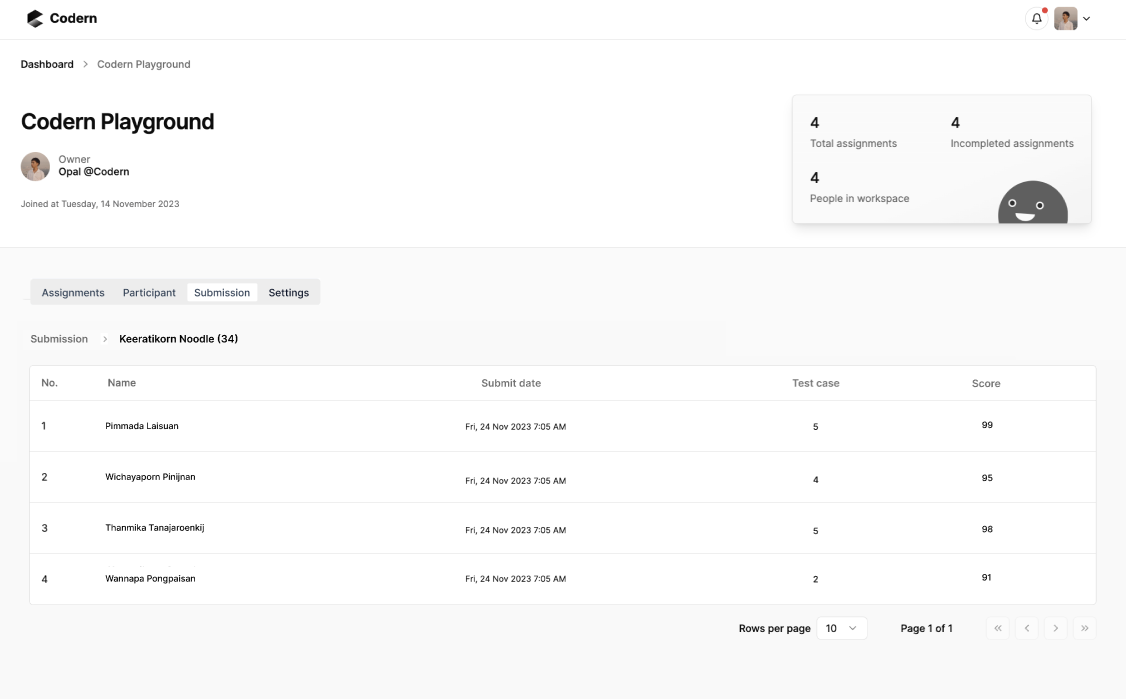
\includegraphics[width=15cm]{figure/ui/ui-assign8.png}}
        \caption[ส่วนประสานต่อผู้ใช้ หน้ารายชื่อสมาชิกห้องเรียนที่ได้ส่งคำตอบของโปรแกรมเข้ามาใน Workspace ของผู้ดูเเลระบบ]{ส่วนประสานต่อผู้ใช้ หน้ารายชื่อสมาชิกห้องเรียนที่ได้ส่งคำตอบของโปรแกรมนั้น ๆ เข้ามาใน Workspace ของผู้ดูเเลระบบ}
        \label{fig:ui-org-assign6}
    \end{figure}
    \begin{flushleft}
    ภายในหน้าดังกล่าว จะแสดงรายชื่อสมาชิกทั้งหมดที่ได้ทำการส่งคำตอบของโปรแกรมนั้น ๆ เข้ามาใน Workspace แล้วดังรูปที่ ~\ref{fig:ui-org-assign6} และจะแสดงรายละเอียดวันเวลาที่ส่งคำตอบเข้ามา จำนวนเทสเคสที่ถูกต้อง และผลคะแนนที่ได้ของโปรแกรมนั้น ๆ ผู้ดูเเลระบบจะสามารถกดเข้าไปในชื่อผู้ใช้คนนั้น ๆ เพื่อดูคำตอบโปรแกรมที่ผู้ใช้คนนั้น ๆ เข้ามาได้ ทั้งผู้ดูแลยังสามารถแสดงความคิดเห็นของตนส่งให้ผู้ใช้คนนั้น ๆ ได้อีกด้วย ซึ่งรายละเอียดหน้าดังกล่าวจะปรากฏดังรูปที่ ~\ref{fig:ui-org-code3}
    \end{flushleft}
    \pagebreak


    %%%%%%%%%%% ORGANIZER COMMENT CODE %%%%%%%%%%%
    \begin{figure}[H]
    \centering
        \fbox{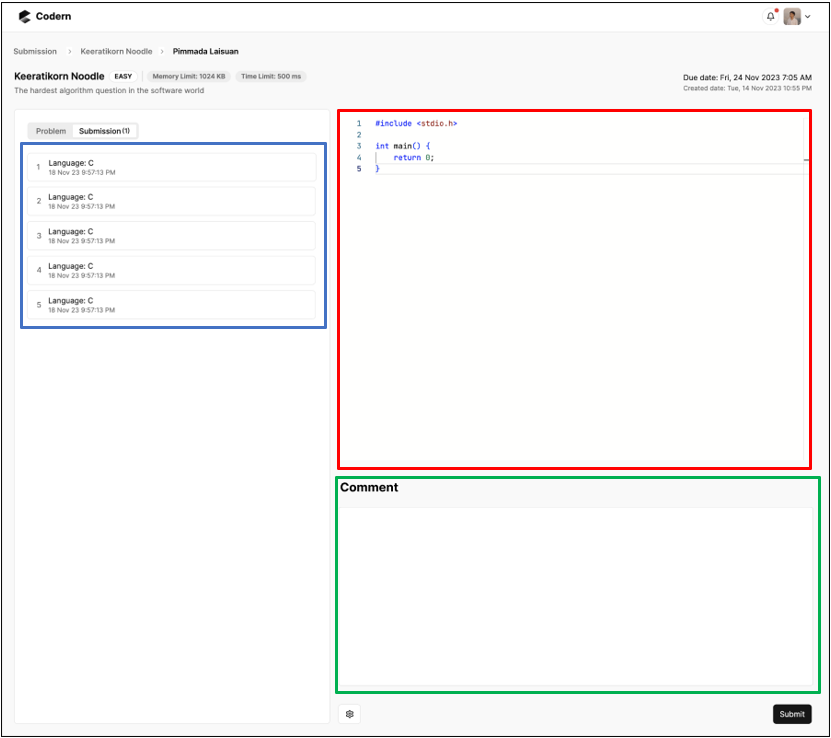
\includegraphics[width=15cm]{figure/ui/ui-code3.png}}
        \caption[ส่วนประสานต่อผู้ใช้ หน้าแสดงคำตอบของโปรแกรมที่ผู้ใช้ได้ส่งเข้ามาใน Workspace ของผู้ดูเเลระบบ]{ส่วนประสานต่อผู้ใช้ หน้าแสดงคำตอบของโปรแกรมที่ผู้ใช้ได้ส่งเข้ามาใน Workspace ของผู้ดูเเลระบบ}
        \label{fig:ui-org-code3}
    \end{figure}
    \begin{flushleft}
    หลังจากเข้ามาแล้ว ภายในหน้านี้จะแสดงคำตอบของโปรแกรมที่ผู้ใช้คนนั้น ๆ ได้ส่งเข้ามาใน Workspace ดังรูปที่ ~\ref{fig:ui-org-code3} โดยรายละเอียดจะแบ่งได้เป็นสามส่วนหลักคือ รายการคำตอบโปรแกรมของแต่ละเทสเคสที่ผู้ใช้ได้ส่งเข้ามา (ตรงกรอบสีน้ำเงินทางซ้ายมือรูปที่~\ref{fig:ui-org-code3}) เมื่อกดที่รายการคำตอบแล้ว จะแสดงคำตอบโปรแกรมของรายการนั้น ๆ ในกล่อง (ตรงกรอบสีแดงทางขวาบนรูปที่~\ref{fig:ui-org-code3}) และทางด้านขวาล่างจะมีพื้นที่สำหรับให้ผู้ดูแลแสดงความคิดเห็นของตน (ตรงกรอบสีเขียวทางขวาล่างรูปที่~\ref{fig:ui-org-code3}) ซึ่งเมื่อกดปุ่ม "Submit" ทางขวาล่างสุดแล้ว ความคิดเห็นก็จะถูกส่งไปยังผู้ใช้คนนั้น ๆ
    \end{flushleft}
    \pagebreak


    %%%%%%%%%%% ASSIGN SETTINGS %%%%%%%%%%%
    \hypertarget{ui-org-assign-settings1}{
        \begin{figure}[H]
        \centering
            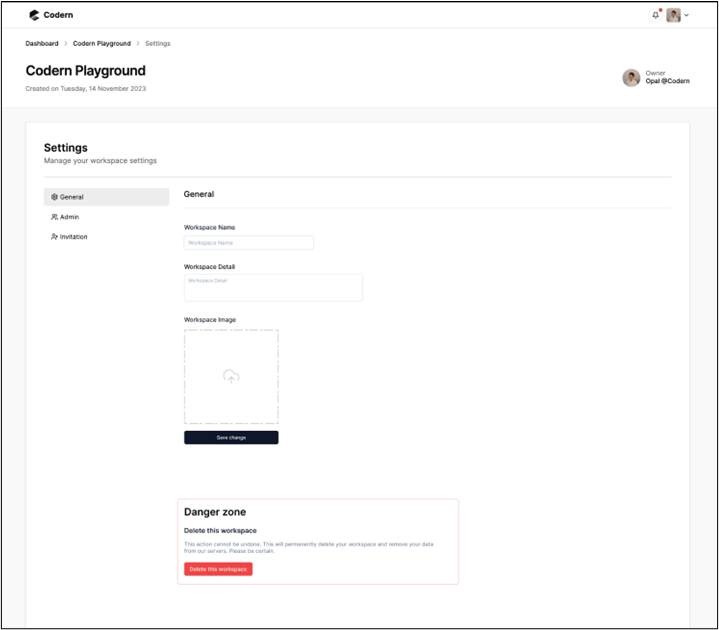
\includegraphics[width=15cm]{figure/ui/ui-assign-settings1.png}
            \caption[ส่วนประสานต่อผู้ใช้ หน้าตั้งค่า Workspace ของผู้ดูเเลระบบ (1)]{ส่วนประสานต่อผู้ใช้ หน้าตั้งค่า Workspace ใน Section "General" ในมุมมองของผู้ดูเเลระบบ}
            \label{fig:ui-org-assign-settings1}
        \end{figure}
    }
        
    \begin{flushleft}
     หลังจากกดตรง Tab ตรง "Settings" (ตรงกรอบ C รูปที่~\ref{fig:ui-org-assign1} ซึ่งมีเเต่ผู้ดูเเลระบบเท่านั้นที่จะเห็น) หน้าในรูปที่~\ref{fig:ui-org-assign-settings1} จะปรากฎขึ้นมา ซึ่งหน้าข้างต้นเป็นหน้าสำหรับตั้งค่าข้อมูลต่าง ๆ ภายในห้องเรียนหรือกลุ่มเรียนนั้น ๆ ซึ่งมีเฉพาะผู้ดูเเลเท่านั้นที่จะสามารถเข้าไปดูเเละเเก้ไขได้เท่านั้น โดยจะแบ่งเป็น 3 ส่วนย่อย ประกอบไปด้วย General settings ซึ่งจะเป็นเมนูแรกสุดดังภาพที่~\ref{fig:ui-org-assign-settings1} ตามมาด้วย Admin settings และ Invitation settings ดังภาพที่~\ref{fig:ui-org-assign-settings2} และภาพที่~\ref{fig:ui-org-assign-settings3} ตามลำดับ
    \end{flushleft}
    \begin{flushleft}
    โดย General settings ดังภาพที่~\ref{fig:ui-org-assign-settings1} จะเป็นหน้าสำหรับการแก้ไขข้อมูลทั่วไปของห้องเรียนนั้น ๆ เช่น ชื่อของห้องเรียน รายละเอียดของห้องเรียน หรือ รูปภาพที่แสดง และที่สำคัญยังสามารถลบห้องเรียนนั้น ๆ ได้เมื่อกดที่ปุ่ม Delete this workspace ภายใน Danger zone ซึ่งการลบห้องเรียนนั้นจะเป็นการลบอย่างถาวร ข้อมูลทั้งหมดจะถูกลบโดยไม่สามารถกู้คืนได้อีก 
    \end{flushleft}

    %%%%%%%%%%% ASSIGN SETTINGS - ADMIN %%%%%%%%%%%
    \hypertarget{ui-org-assign-settings2}{
        \begin{figure}[H]
        \centering
            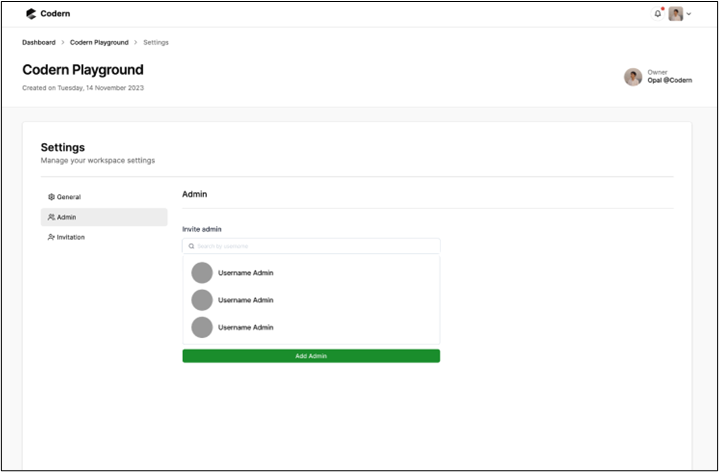
\includegraphics[width=15cm]{figure/ui/ui-assign-settings2.png}
            \caption[ส่วนประสานต่อผู้ใช้ หน้าตั้งค่า Workspace ของผู้ดูเเลระบบ (2)]{ส่วนประสานต่อผู้ใช้ หน้าตั้งค่า Workspace ใน Section "Admin" ในมุมมองของผู้ดูเเลระบบ}
            \label{fig:ui-org-assign-settings2}
        \end{figure}
    }

    \pagebreak
    \begin{flushleft}
    ในของ "Admin" Settings ดังภาพที่~\ref{fig:ui-org-assign-settings2} จะเป็นหน้าสำหรับการเพิ่มแอดมินหรือผู้ดูแลเข้าสู่ห้องเรียนนั้น ๆ โดยจะประกอบด้วยกล่องค้นหา หากค้นหาพบคนที่ต้องการแล้ว เมื่อกดปุ่ม "Add admin" จะเป็นการเพิ่มผู้ดูแลคนนั้น ๆ เข้าสู่ห้องเรียน
    \end{flushleft}
    
    %%%%%%%%%%% ASSIGN SETTINGS - INVITATION %%%%%%%%%%%
    \hypertarget{ui-org-assign-settings3}{
        \begin{figure}[H]
        \centering
            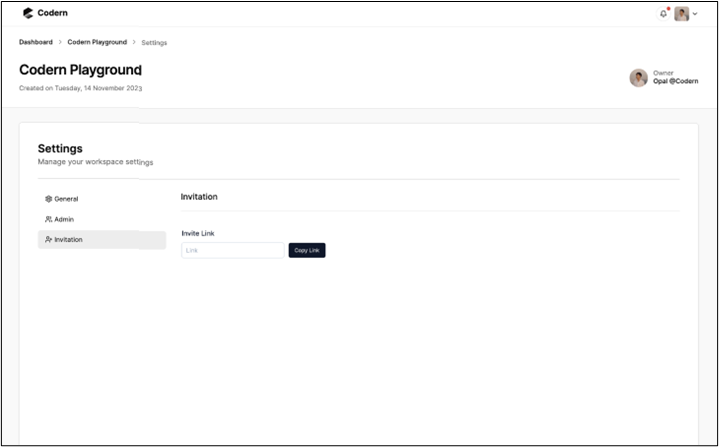
\includegraphics[width=15cm]{figure/ui/ui-assign-settings3.png}
            \caption[ส่วนประสานต่อผู้ใช้ หน้าตั้งค่า Workspace ของผู้ดูเเลระบบ (3)]{ส่วนประสานต่อผู้ใช้ หน้าตั้งค่า Workspace ใน Section "Invitation" ในมุมมองของผู้ดูเเลระบบ}
            \label{fig:ui-org-assign-settings3}
        \end{figure}
    }
    \begin{flushleft}
    สุดท้ายในส่วนของ "Invitation" Settings ดังภาพที่~\ref{fig:ui-org-assign-settings3} เป็นหน้าสำหรับการเชิญผู้ใช้ทั่วไปเข้าสู่ห้องเรียนนั้น ๆ โดยตัวผู้ดูแล ซึ่งทำได้โดยจะมีการสร้างรหัสเชิญขึ้น หากกดปุ่ม "Copy link" จะเป็นการคัดลอกรหัสเชิญไปยังคลิปบอร์ด และเมื่อผู้ใช้กรอกรหัสดังกล่าวลงในกล่อง "Join with code" ในภาพที่~\ref{fig:ui-dashboard4} และกดปุ่ม "Join" จะเป็นการเข้าร่วมห้องเรียนนั้น ๆ 
    \end{flushleft}

    \begin{flushleft}
    ถ้าหากกดรายการการบ้าน โจทย์ปัญหา มาสักรายการ (ในรูปที่~\ref{fig:ui-assign1}) ก็จะนำพามาสู่หน้าโจทย์ปัญหาในรูปที่~\ref{fig:ui-code1} โดยในหน้านี้ในโซนที่ 1 จะเป็นช่องแผงเขียนโปรแกรม สามารถที่จะเขียนโปรแกรมภาษาคอมพิวเตอร์ในโซนนี้ได้ ในโซนที่สอง จะเป็นแสดงรายละเอียดของโจทย์ตั้งแต่เนื้อหาโจทย์ ไปจนถึงจำนวนหน่วยความจำที่ใช้ได้ (Memory Limit) และระยะเวลาที่ใช้ในการหาคำตอบ (Runtime Limit) ถ้าหากต้องการส่งก็สามารถที่จะกดปุ่ม “Submit” ที่กรอบน้ำเงิน A เพื่อส่งงานเขียนโปรแกรมไปให้ตรวจ และอีกทั้งก่อนส่ง ก็ยังสามารถที่จะตั้งค่าและเลือก compiler ที่ต้องการจะใช้ในการตรวจงานเขียนโปรแกรมดังกล่าวได้ที่ Dropdown ที่กรอบน้ำเงิน B หลังจากผู้ใช้กดส่งไปตรวจแล้ว สามารถติดตามผลได้ในรายการ submission ซึ่งสามารถกดดูได้ตรงกรอบสีเขียว C ในรูปที่~\ref{fig:ui-code1} 
    \end{flushleft}
    \begin{flushleft}
    หลังจากกดเลือก Tab ชื่อ "Submission" เเผงแสดงผลเนื้อหาโจทย์ จะถูกเปลี่ยนมาเป็นรายการผลส่งการตรวจทั้งหมด ในโซนกรอบแดงที่ 1 ในรูป~\ref{fig:ui-code2} โดยในรายการก็จะแสดงรายละเอียดการส่งแต่ละครั้งที่ผู้ใช้ส่ง มีรายละเอียดต่าง ๆ อาทิเช่น ภาษาที่ส่งไปตรวจ และผลการตรวจของแต่ละ Test Case (ถ้า PASS แปลว่า output ของโปรแกรมที่เขียนให้ผลตรงตาม Test Case ที่โจทย์ข้อนี้ตั้งไว้, แต่ถ้า FAIL ก็จะแสดงว่า output ของโปรแกรมที่เขียนไม่ได้ให้ผลตรงตาม Test Case ที่โจทย์ข้อนี้ตั้งไว้)
    \end{flushleft}
    
    %%%%%%%%%%% CODE PAGE - PROBLEM %%%%%%%%%%%
    \hypertarget{ui-code1}{
        \begin{figure}[H]
        \centering
        \fbox{
            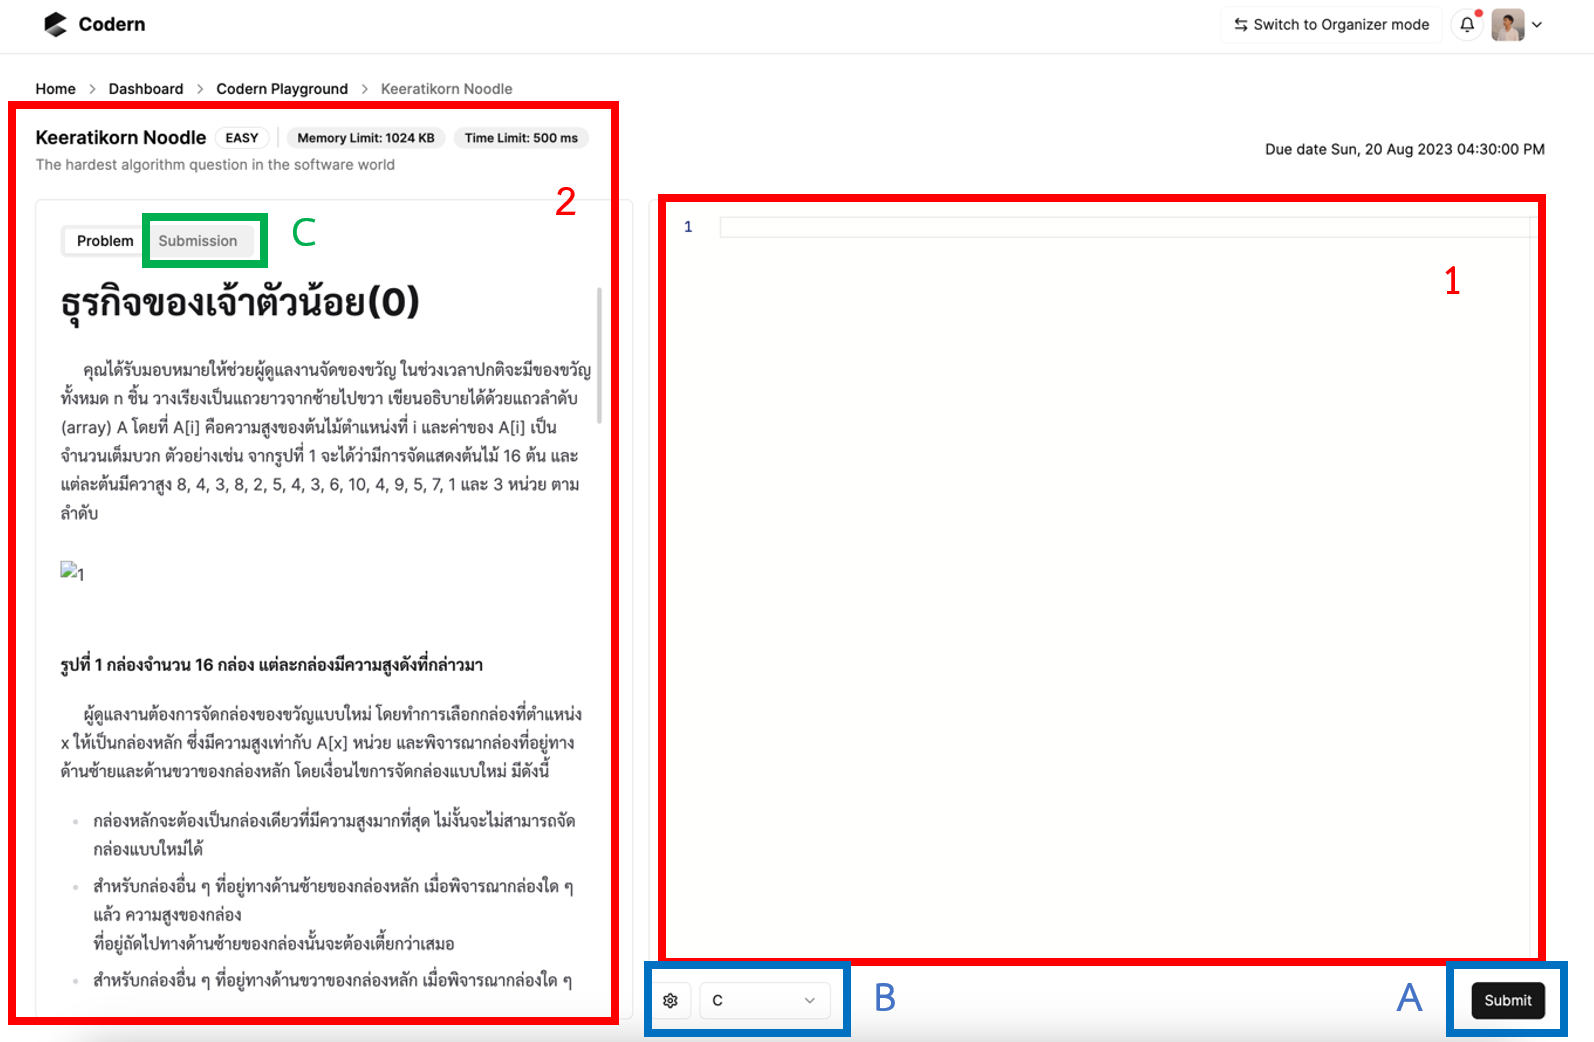
\includegraphics[width=15cm]{figure/ui/ui-code1.png}
        }
            \caption[ส่วนประสานต่อผู้ใช้ หน้าแผงเขียนโปรแกรม (1)]{ส่วนประสานต่อผู้ใช้ หน้าโจทย์ปัญหาและแผงเขียนโปรแกรม}
            \label{fig:ui-code1}
        \end{figure}
    }
    %%%%%%%%%%% CODE PAGE - SUBMISSION %%%%%%%%%%%
    \hypertarget{ui-code2}{
        \begin{figure}[H]
        \centering
        \fbox{
            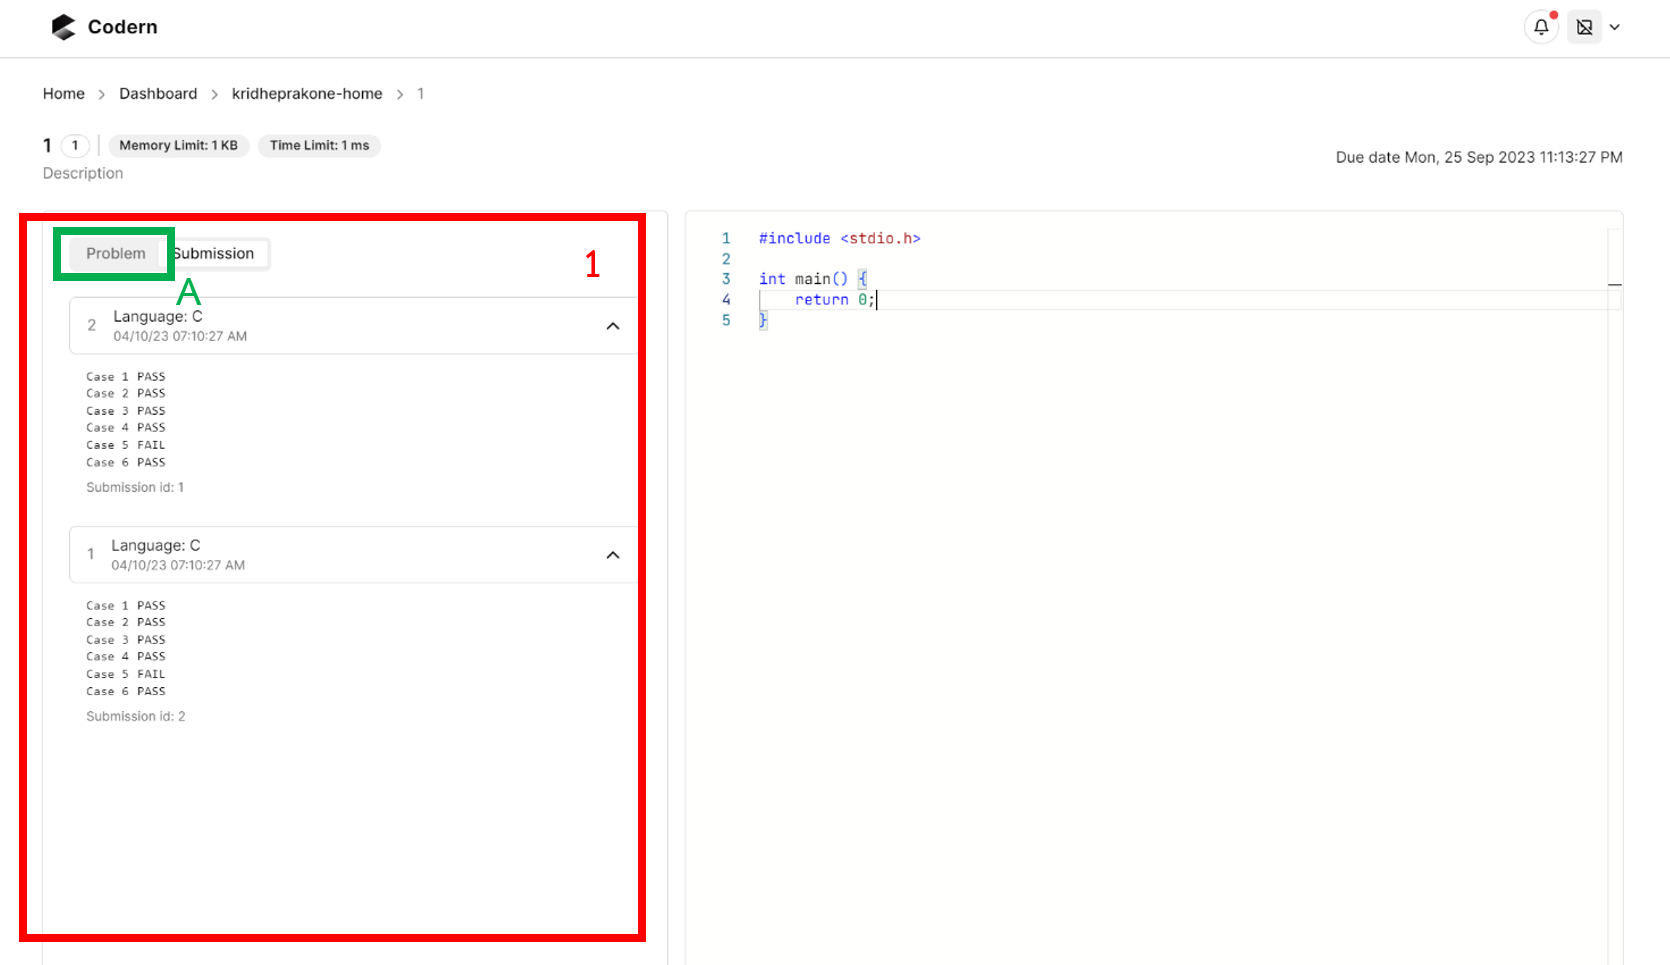
\includegraphics[width=15cm]{figure/ui/ui-code2.png}
        }
            \caption[ส่วนประสานต่อผู้ใช้ หน้าแผงเขียนโปรแกรม (2)]{ส่วนประสานงานต่อผู้ใช้ หน้าโจทย์ปัญหาและแผงเขียนโปรแกรม พร้อมรายการส่งเเละผลการตรวจทั้งหมด}
            \label{fig:ui-code2}
        \end{figure}
    }
    
    %%%%%%%%%%% USER ARCHIVE %%%%%%%%%%%
    \hypertarget{ui-archive1}{
        \begin{figure}[H]
        \centering
        % \fbox{
            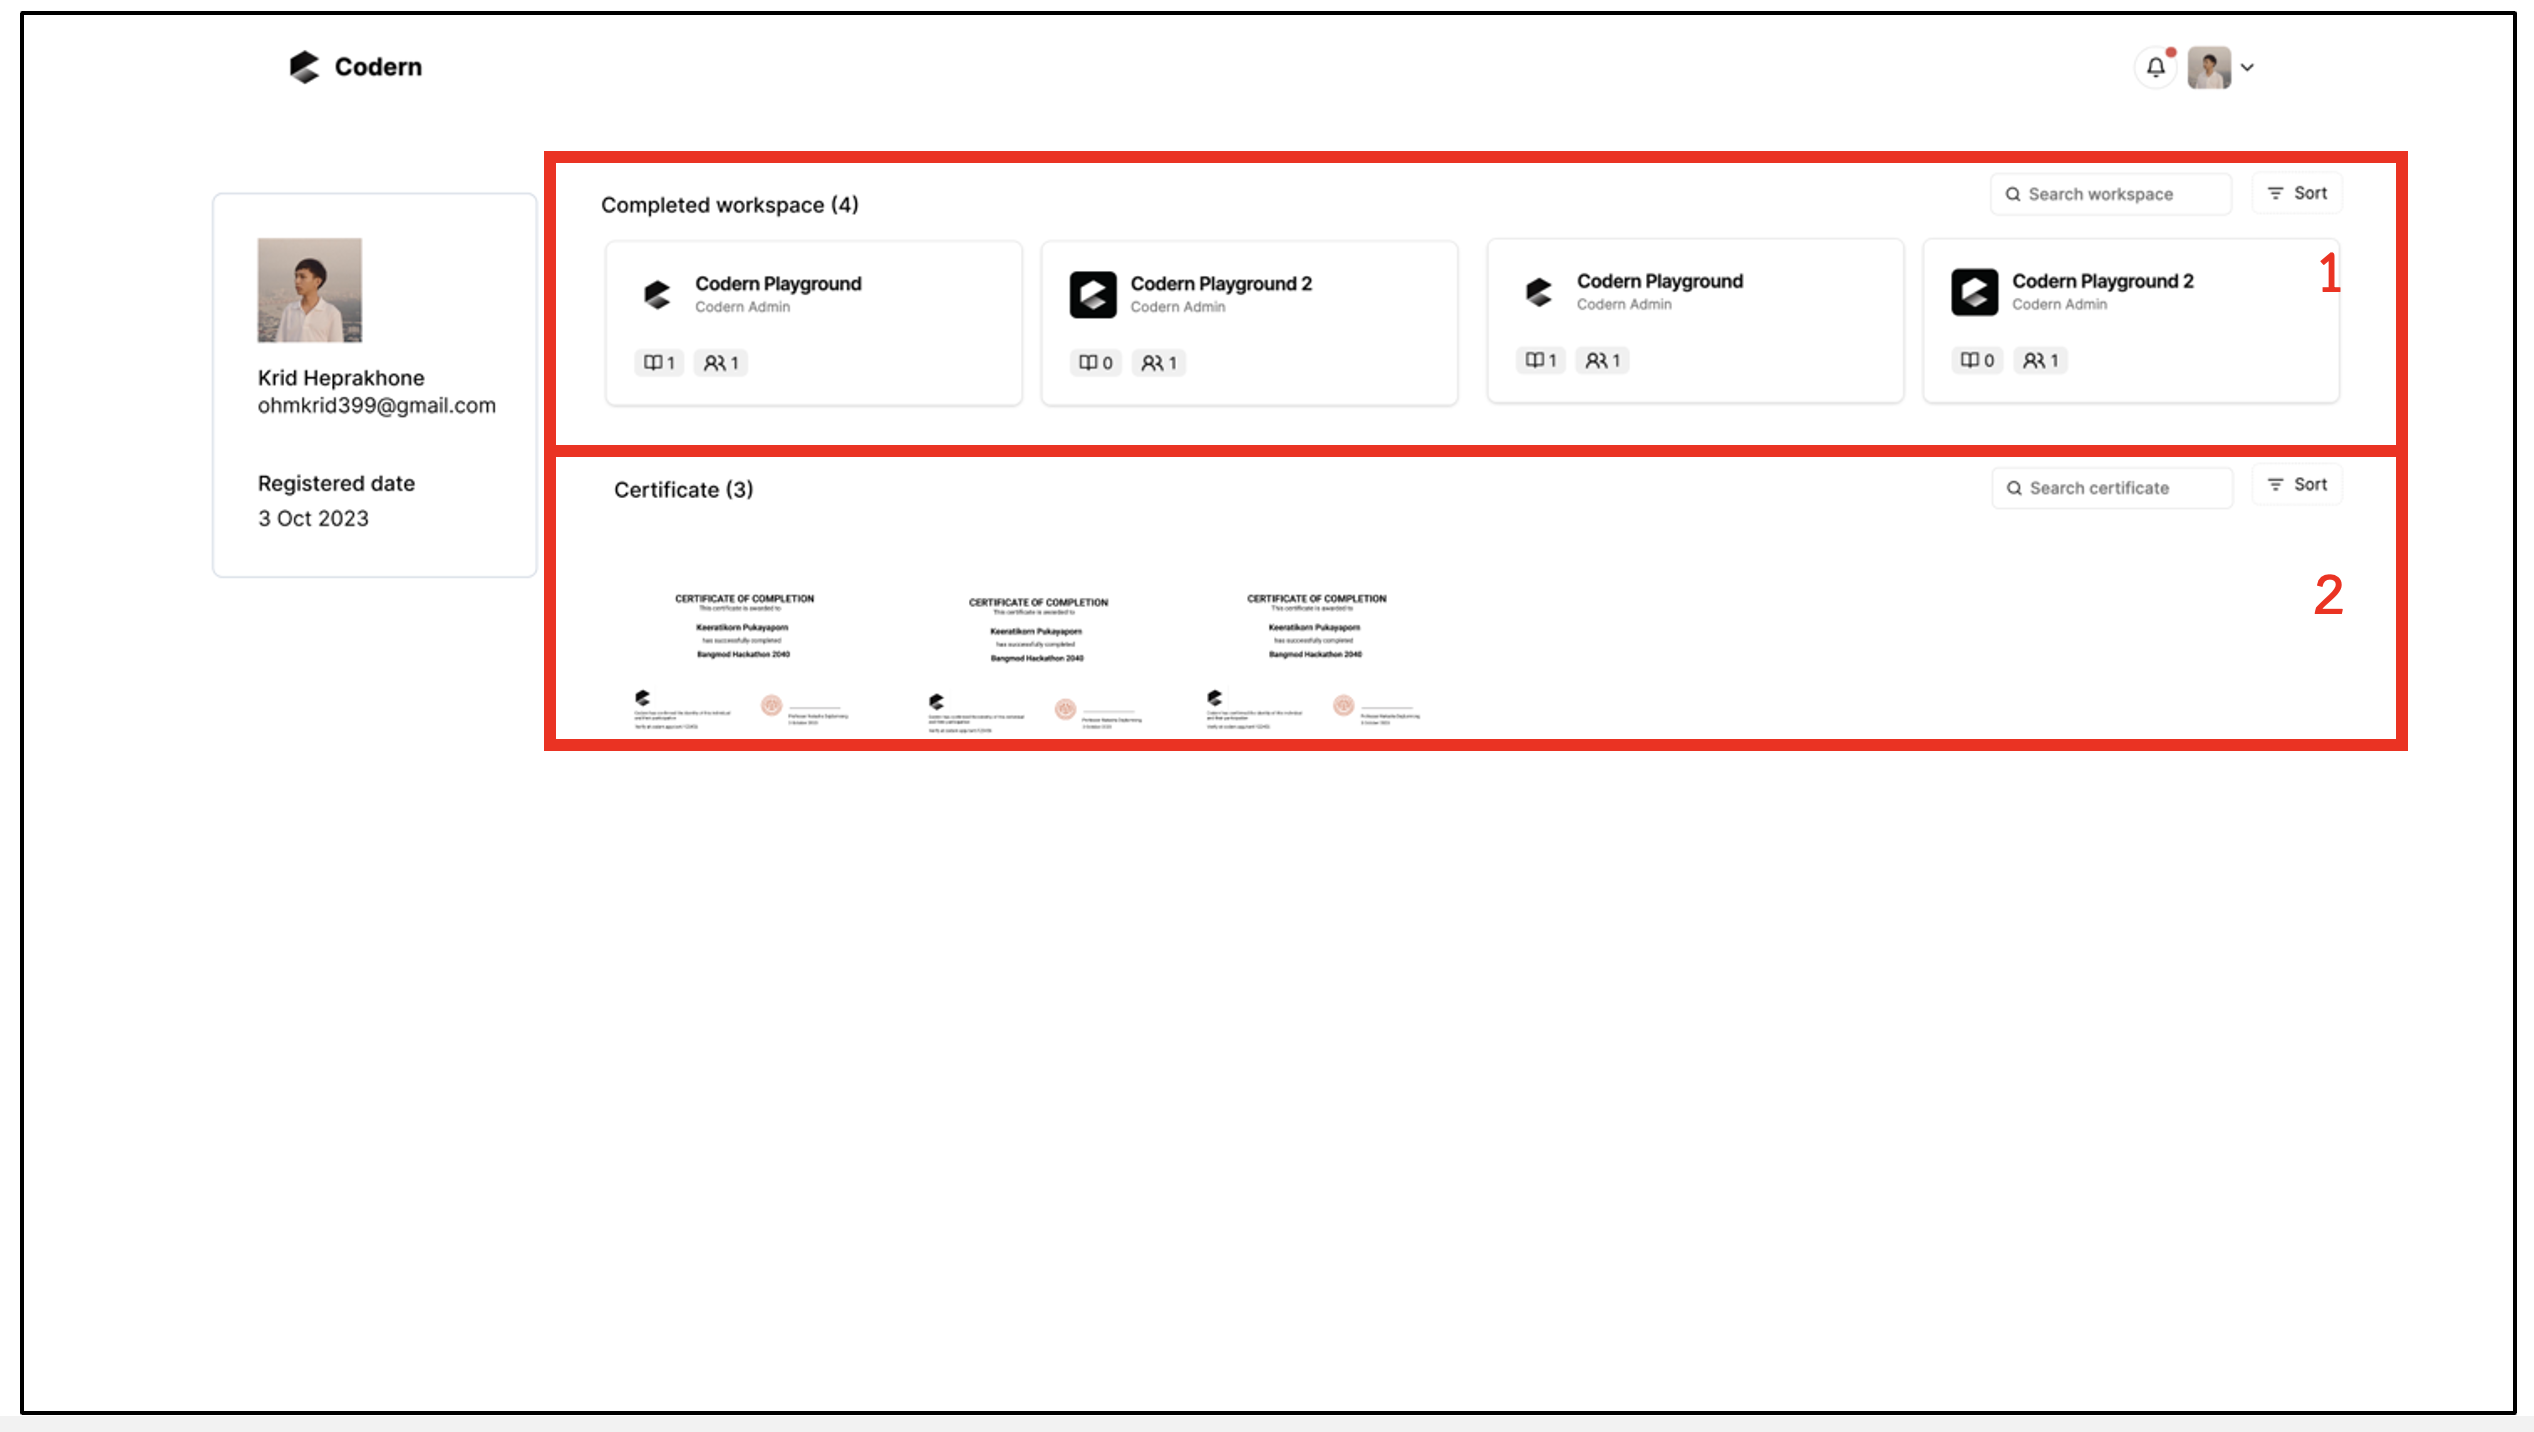
\includegraphics[width=15cm]{figure/ui/ui-archive1.png}
        % }
            \caption[ส่วนประสานงานต่อผู้ใช้ หน้าแสดงข้อมูลของผู้ใช้เก่า]{ส่วนประสานงานต่อผู้ใช้ หน้าแสดงข้อมูล ประวัติการใช้งาน และเกียรติบัตรทั้งหมด ของผู้ใช้เก่า}
            \label{fig:ui-archive1}
        \end{figure}
    }
    
    \begin{flushleft}
    ในอีกโดเมนเเยกจากระบบหลัก (ดูแผนผังการนำทางระหว่างหน้าของเว็บไซต์ ในรูปที่~\ref{fig:nav-map}) หน้าแสดงข้อมูลและประวัติการใช้งานของผู้ใช้เก่า (ในรูปที่~\ref{fig:ui-archive1}) เช่น นักเรียนหรือนักศึกษาที่ได้จบการศึกษาไปแล้ว เป็นต้น 
    \end{flushleft}
    \begin{flushleft}
    ผู้ใช้ทั่วไป (ไม่จำเป็นต้องมีบัญชีบนซอฟต์แวร์ ณ เวลานั้น) สามารถที่จะเข้ามาค้นดูประวัติ ข้อมูลการใช้งาน ภาระงานที่ได้ทำ ห้องหรือกลุ่มเรียนที่เคยได้เข้าร่วม (โซนกรอบแดงที่ 1) พร้อมทั้งค้นเอาเกียรติบัตร (โซนกรอบแดงที่ 2) ไปพิมพ์ใช้งานต่อได้ (เกียรติบัตรจะถูกสร้างขึ้นแก่ผู้ใช้ทุกคนก็ต่อเมื่อเจ้าของห้อง ปิดห้องหรือกลุ่มเรียน) สำหรับยื่นหรือให้การศึกษาต่อ ใช้สมัครงานต่อไปก็ได้
    \end{flushleft}
    
\pagebreak
\newpage
\section{โครงสร้างฐานข้อมูล}
    \begin{flushleft}
    จากรูปที่~\ref{fig:database} ด้านล่าง เป็นแผนภาพแสดงฐานข้อมูลของซอฟต์แวร์ที่ทางคณะผู้จัดทำได้ออกแบบไว้เบื้องต้น ฐานข้อมูลดังกล่าวเป็น Relation Database Management System ที่จะเก็บข้อมูลบนซอฟต์แวร์ตั้งแต่ข้อมูลผู้ใช้ จนไปถึงข้อมูลกลุ่มห้อง/ห้องเรียน ข้อมูลโจทย์ ทั้งเนื้อหาของโจทย์พร้อมทั้ง Test Case ของโจทย์แต่ละข้อ
    \end{flushleft}
    %%%%%%%%%%% DATABASE ER DIAGRAM %%%%%%%%%%%
    \hypertarget{database}{
            \begin{figure}[H]
            \centering
            % \fbox{
                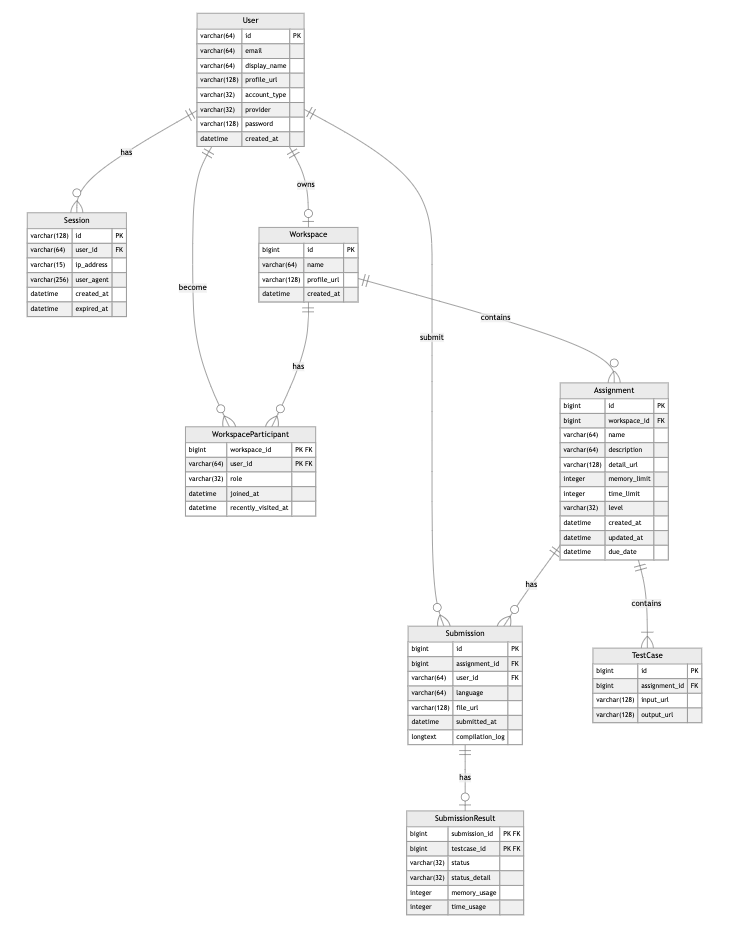
\includegraphics[width=15cm]{figure/diagram/database-v3.png}
            % }
                \caption[แผนภาพฐานข้อมูล]{แผนภาพฐานข้อมูล วาดด้วย \href{https://mermaid.js.org/}{Mermaid JS}}
                \label{fig:database}
            \end{figure}
        }

    \pagebreak
    \begin{flushleft}
     ในระบบฐานข้อมูลนี้ ประกอบด้วยตารางดังต่อไปนี้
    \end{flushleft}
    \begin{enumerate}
        %%%%%%%%%%% USER RELATIONSHIP %%%%%%%%%%%    
        \item \textbf{User}
            เป็นตารางที่เก็บข้อมูลของผู้ใช้แต่ละคน เช่นอีเมลล์, ชื่อ-นามสกุลขของผู้ใช้ เป็นต้น จากความสัมพันธ์ของตารางดังกล่าว กับตารางอื่น ๆ สามารถสรุปความสัมพันธ์ได้ดังนี้
            \begin{itemize}
                \item จากรูปที่~\ref{fig:db-user-session} ผู้ใช้สามารถที่จะเข้าสู่ระบบได้หลายเครื่องพร้อม ๆ กัน ก็คือผู้ใช้เข้าสู่ระบบได้ (has) หลาย Session พร้อมกัน
                    \begin{figure}[H]
                        \centering 
                        \begin{tikzpicture}[auto,node distance=1.5cm]
                            % First Entity
                            \node[entity] (node1) {User};
                            % [grow=up,sibling distance=3cm]
                            % child {node[attribute] {Attribute 1}}
                            % child {node[attribute] {Attribute 2}}
                            % child[grow=left,level distance=3cm] {node[attribute] {Attribute 3}};
                            % Relationship
                            \node[relationship] (rel1) [right = of node1] {has};
                            % Second Entity
                            \node[entity] (node2) [right = of rel1]	{Session};
                            % Draw an edge between rel1 and node1; rel1 and node2
                            \path (rel1) edge node {\(1\)-\(1\)} 
                            (node1) edge node {\(1\)-\(m\)}	(node2);
                        \end{tikzpicture}
                        \caption[แผนผังแสดงความสัมพันธ์ระหว่างตาราง User และ Session]{แผนผังแสดงความสัมพันธ์ระหว่างตาราง User และ Session}
                        \label{fig:db-user-session}
                    \end{figure}
                \item จากรูปที่~\ref{fig:db-user-workspace} ผู้ใช้สามารถที่จะครอบครอง (owns) Workspace ได้มากกว่า 1 Workspace
                    \begin{figure}[H]
                        \centering 
                        \begin{tikzpicture}[auto,node distance=1.5cm]
                            % First Entity
                            \node[entity] (node1) {User};
                            % Replationship
                            \node[relationship] (rel1) [right = of node1] {owns};
                            % Second Entity
                            \node[entity] (node2) [right = of rel1]	{Workspace};
                            % Draw an edge between rel1 and node1; rel1 and node2
                            \path (rel1) edge node {\(1\)-\(1\)} 
                            (node1) edge node {\(0\)-\(m\)}	(node2);
                        \end{tikzpicture}
                        \caption[แผนผังแสดงความสัมพันธ์ระหว่างตาราง User และ Workspace]{แผนผังแสดงความสัมพันธ์ระหว่างตาราง User และ Workspace}
                        \label{fig:db-user-workspace}
                    \end{figure}
                \item จากความสัมพันธ์ในรูป~\ref{fig:db-user-workspace_participant} ผู้ใช้สามารถที่จะเป็นคนเข้าร่วม (join workspace) ในกลุ่มเรียนหรือห้องเรียน (หรือ Workspace Participant) ได้มากกว่า 1 ห้องเรียนหรือกลุ่มเรียน หรือ Workspace
                    \begin{figure}[H]
                        \centering 
                        \begin{tikzpicture}[auto,node distance=1.5cm]
                            % First Entity
                            \node[entity] (node1) {User};
                            % Relationship
                            \node[relationship] (rel1) [right = of node1] {becomes};
                            % Second Entity
                            \node[entity] (node2) [right = of rel1]	{WorkspaceParticipant};
                            % Draw an edge between rel1 and node1; rel1 and node2
                            \path (rel1) edge node {\(1\)-\(1\)} 
                            (node1) edge node {\(0\)-\(m\)}	(node2);
                        \end{tikzpicture}
                        \caption[แผนผังแสดงความสัมพันธ์ระหว่างตาราง User และ WorkspaceParticipant]{แผนผังแสดงความสัมพันธ์ระหว่างตาราง User และ WorkspaceParticipant}
                        \label{fig:db-user-workspace_participant}
                    \end{figure}
                    \item จากรูปที่~\ref{fig:db-user-submission} ผู้ใช้สามารถที่จะส่ง (submit) ได้มากกว่า 1 ห้องเรียนหรือกลุ่มเรียน หรือ Workspace
                    \begin{figure}[H]
                        \centering 
                        \begin{tikzpicture}[auto,node distance=1.5cm]
                            % First Entity
                            \node[entity] (node1) {User};
                            % Relationship
                            \node[relationship] (rel1) [right = of node1] {submit};
                            % Second Entity
                            \node[entity] (node2) [right = of rel1]	{Submission};
                            % Draw an edge between rel1 and node1; rel1 and node2
                            \path (rel1) edge node {\(1\)-\(1\)} 
                            (node1) edge node {\(0\)-\(m\)}	(node2);
                        \end{tikzpicture}
                        \caption[แผนผังแสดงความสัมพันธ์ระหว่างตาราง User และ Submission]{แผนผังแสดงความสัมพันธ์ระหว่างตาราง User และ Submission}
                        \label{fig:db-user-submission}
                    \end{figure}
            \end{itemize}
        %%%%%%%%%%% SESSION RELATIONSHIP %%%%%%%%%%%        
        \item \textbf{Session}
            เป็นตารางที่จะเก็บข้อมูล Session หรือข้อมูลเครื่อง ข้อมูลช่องทางที่ผู้ใช้เข้าสู่ระบบ สามารถสรุปความสัมพันธ์ได้ดังนี้
                \begin{itemize}
                    \item ถึงเเม้ผู้ใช้หนึ่งท่านสามารถที่จะมีได้หลาย Session คือผู้ใช้สามารถเข้าสู่ระบบได้หลายเครื่องพร้อมก่อน แต่ Session เป็นของผู้ใช้แค่คนเดียวเท่านั้นตามรูปที่~\ref{fig:db-user-session}
                \end{itemize}
        %%%%%%%%%%% WORKSPACE RELATIONSHIP %%%%%%%%%%%
        \item \textbf{Workspace}
            เป็นตารางที่สร้างขึ้นมาเก็บข้อมูลห้องเรียนหรือกลุ่มเรียน (Workspace) มีความสัมพันธ์กับตารางอื่นดังต่อไปนี้
                \begin{itemize}
                    \item จากรูปที่~\ref{fig:db-user-session} ห้องเรียนหรือกลุ่มเรียนมีผู้ใช้ที่เป็นเจ้าของห้องได้เพียงแค่หนึ่งท่านเท่านั้น ตามในรูปเดิม รูปที่~\ref{fig:db-user-workspace}
                    \item ในหนึ่งกลุ่มเรียนหรือห้องเรียน สามารถมี (has) ผู้เข้าร่วมหรือ Workspace Participant ได้หลายคน ตามในรูปที่~\ref{fig:db-workspace-workspace_participant}
                    \begin{figure}[H]
                        \centering 
                        \begin{tikzpicture}[auto,node distance=1.5cm]
                            % First Entity
                            \node[entity] (node1) {Workspace};
                            % Relationship
                            \node[relationship] (rel1) [right = of node1] {has};
                            % Second Entity
                            \node[entity] (node2) [right = of rel1]	{WorkspaceParticipant};
                            % Draw an edge between rel1 and node1; rel1 and node2
                            \path (rel1) edge node {\(1\)-\(1\)} 
                            (node1) edge node {\(0\)-\(m\)}	(node2);
                        \end{tikzpicture}
                        \caption[แผนผังแสดงความสัมพันธ์ระหว่างตาราง Workspace และ WorkspaceParticipant]{แผนผังแสดงความสัมพันธ์ระหว่างตาราง Workspace และ WorkspaceParticipant}
                        \label{fig:db-workspace-workspace_participant}
                    \end{figure}
                    \item จากรูปที่~\ref{fig:db-workspace-assignment} ในหนึ่งกลุ่มเรียนหรือห้องเรียน สามารถที่จะมี (contains) โจทย์ปัญหา การบ้านหรือข้อสอบ (Assignment) ได้หลายรายการ 
                    \begin{figure}[H]
                        \centering 
                        \begin{tikzpicture}[auto,node distance=1.5cm]
                            % First Entity
                            \node[entity] (node1) {Workspace};
                            % Relationship
                            \node[relationship] (rel1) [right = of node1] {contains};
                            % Second Entity
                            \node[entity] (node2) [right = of rel1]	{Assignment};
                            % Draw an edge between rel1 and node1; rel1 and node2
                            \path (rel1) edge node {\(1\)-\(1\)} 
                            (node1) edge node {\(0\)-\(m\)}	(node2);
                        \end{tikzpicture}
                        \caption[แผนผังแสดงความสัมพันธ์ระหว่างตาราง Workspace และ Assignment]{แผนผังแสดงความสัมพันธ์ระหว่างตาราง Workspace และ Assignment}
                        \label{fig:db-workspace-assignment}
                    \end{figure}
                \end{itemize}
        %%%%%%%%%%% WORKSPACE_PARTICIPANT RELATIONSHIP %%%%%%%%%%%
        \item \textbf{WorkspaceParticipant}
            เป็นตารางที่สร้างขึ้นมาเก็บข้อมูลของผู้เข้าร่วมในเเต่ละห้องเรียนหรือกลุ่มเรียน (Workspace) มีความสัมพันธ์กับตารางอื่นดังต่อไปนี้
                \begin{itemize}
                    \item อ้างอิงจากรูปที่~\ref{fig:db-user-workspace_participant} สถานะของการเป็นผู้เข้าร่วมห้องใดห้องหนึ่งถูก เป็นของผู้ใช้เพียงหนึ่งท่านเท่านั้น
                    \item สถานะของการเป็นผู้เข้าร่วมห้องใดห้องหนึ่งถูก เป็นสถานะของห้องเรียนหรือกลุ่มเรียนเดียวเท่านั้น ตามความสัมพันธ์ในรูปที่~\ref{fig:db-workspace-workspace_participant}
                \end{itemize}
        %%%%%%%%%%% ASSIGNMENT RELATIONSHIP %%%%%%%%%%%
        \item \textbf{Assignment}
            เป็นตารางที่สร้างขึ้นมาเก็บข้อมูลและรายละเอียดของการบ้าน ข้อสอบและโจทย์ปัญหาทั้งหมด (Assignment) สามารถสรุปความสัมพันธ์กับตารางอื่นได้ดังต่อไปนี้
                \begin{itemize}
                    \item ดูจากรูปที่~\ref{fig:db-workspace-assignment} การบ้าน ข้อสอบและโจทย์ปัญหาเป็นของ Workspace เดียวเท่านั้น
                    \item โจทย์ปัญหา การบ้านหรือข้อสอบแต่ละข้อมี (has) ได้ข้อมูลส่งงาน (Submission) ได้หลายรายการ ตามรูปที่~\ref{fig:db-assignment-submission}
                    \begin{figure}[H]
                        \centering 
                        \begin{tikzpicture}[auto,node distance=1.5cm]
                            % First Entity
                            \node[entity] (node1) {Assignment};
                            % Relationship
                            \node[relationship] (rel1) [right = of node1] {has};
                            % Second Entity
                            \node[entity] (node2) [right = of rel1]	{Submission};
                            % Draw an edge between rel1 and node1; rel1 and node2
                            \path (rel1) edge node {\(1\)-\(1\)} 
                            (node1) edge node {\(0\)-\(m\)}	(node2);
                        \end{tikzpicture}
                        \caption[แผนผังแสดงความสัมพันธ์ระหว่างตาราง Assignment และ Submission]{แผนผังแสดงความสัมพันธ์ระหว่างตาราง Assignment และ Submission}
                        \label{fig:db-assignment-submission}
                    \end{figure}
                    \item โจทย์ปัญหา การบ้านหรือข้อสอบแต่ละข้อมี (contains) ได้หลายกรณีทดสอบหรือเทสเคส (Test Case) ตามในรูปที่~\ref{fig:db-assignment-testcase}
                    \begin{figure}[H]
                        \centering 
                        \begin{tikzpicture}[auto,node distance=1.5cm]
                            % First Entity
                            \node[entity] (node1) {Assignment};
                            % Relationship
                            \node[relationship] (rel1) [right = of node1] {contains};
                            % Second Entity
                            \node[entity] (node2) [right = of rel1]	{TestCase};
                            % Draw an edge between rel1 and node1; rel1 and node2
                            \path (rel1) edge node {\(1\)-\(1\)} 
                            (node1) edge node {\(0\)-\(m\)}	(node2);
                        \end{tikzpicture}
                        \caption[แผนผังแสดงความสัมพันธ์ระหว่างตาราง Assignment และ TestCase]{แผนผังแสดงความสัมพันธ์ระหว่างตาราง Assignment และ TestCase}
                        \label{fig:db-assignment-testcase}
                    \end{figure}
                \end{itemize}
        %%%%%%%%%%% SUBMISSION RELATIONSHIP %%%%%%%%%%%
        \item \textbf{Submission}
            เป็นตารางที่เก็บบันทึกรายการส่งงาน รายละเอียดและข้อมูลไฟล์งานเขียนโปรแกรมที่ผู้ใข้ส่งมาให้ตรวจ มีความสัมพันธ์ดังนี้
                \begin{itemize}
                    \item ดูจากรูปที่~\ref{fig:db-user-submission} ข้อมูลส่งงานหนึ่งรายการ เป็นของผู้ใช้หนึ่งท่านเท่านั้น
                    \item ข้อมูลส่งงานหนึ่งรายการ จะเชื่อมกับโจทย์ปัญหา การบ้านหรือข้อสอบตัวเดียวเท่านั้น อ้่างอิงจากความสัมพันธ์ในรูปที่~\ref{fig:db-assignment-submission}
                    \item ข้อมูลส่งงานหนึ่งรายการ (Submission มีได้ (has) แค่เพียงหนึ่งผลลัพธ์การตรวจเท่านั้น (Submission Result) ตามความสัมพันธ์ในรูปที่~\ref{fig:db-submission-submission_result}
                    \begin{figure}[H]
                        \centering 
                        \begin{tikzpicture}[auto,node distance=1.5cm]
                            % First Entity
                            \node[entity] (node1) {Submission};
                            % Relationship
                            \node[relationship] (rel1) [right = of node1] {has};
                            % Second Entity
                            \node[entity] (node2) [right = of rel1]	{SubmissionResult};
                            % Draw an edge between rel1 and node1; rel1 and node2
                            \path (rel1) edge node {\(1\)-\(1\)} 
                            (node1) edge node {\(0\)-\(1\)}	(node2);
                        \end{tikzpicture}
                        \caption[แผนผังแสดงความสัมพันธ์ระหว่างตาราง Assignment และ TestCase]{แผนผังแสดงความสัมพันธ์ระหว่างตาราง Assignment และ TestCase}
                        \label{fig:db-submission-submission_result}
                    \end{figure}
                \end{itemize}
        %%%%%%%%%%% TEST_CASE RELATIONSHIP %%%%%%%%%%%
        \item \textbf{TestCase}
            เป็นตารางที่เก็บกรณีทดสอบหรือตรวจสอบโปรแกรม หรือเทสเคส (Test Case) ประกอบด้วยความสัมพันธ์ต่อไปนี้
            \begin{itemize}
                    \item ดูจากรูปที่~\ref{fig:db-assignment-testcase} หนึ่งกรณีทดสอบ (Test Case) เชื่อมกับหนึ่งโจทย์ปัญหา ข้อสอบหรือการบ้าน (Assignment) หนึ่งข้อเท่านั้น
            \end{itemize}
        %%%%%%%%%%% SUBMISSION_RESULT RELATIONSHIP %%%%%%%%%%%
        \item \textbf{SubmissionResult}
            เป็นตารางที่เก็บบันทึกผลลัพธ์การตรวจทั้งหมด ประกอบด้วยความสัมพันธ์ดังต่อไปนี้
            \begin{itemize}
                \item จากความสัมพันธ์ในรูปที่~\ref{fig:db-submission-submission_result} ผลลัพธ์การตรวจหนึ่งรายการ (Submission Result) เชื่อมกับแค่หนึ่งข้อมูลส่งงาน (Submission) เท่านั้น
            \end{itemize}
        \end{enumerate}
        
    \pagebreak
    \subsection{พจนานุกรมข้อมูล}
    ในส่วนนี้ จะเป็นพจนานุกรมสำหรับอธิบายตัวแปรและตารางต่าง ๆ ที่อยู่ในแผนภาพฐานข้อมูลในรูปที่ 3.4 ในหัวข้อก่อน
    %%%%%%%%%%% DATA DICTIONARY TABLE %%%%%%%%%%%
    \begin{table}[!h]
        \centering
        \caption{พจนานุกรมข้อมูลของตาราง User}\label{tbl:data-dict-user}
        \begin{tabular}{p{2cm}|p{4cm}p{2cm}p{3cm}p{2cm}} \hline\hline
            Attribute Name & Description & Data Type & Constraints & References \\ \hline\hline
            id & รหัส ID การส่งงาน & bigint & Primary Key & - \\
            assignment\_id & ID ของภาระงานหรือโจทย์ & bigint & Foreign Key, Not Null & Assignment \\
            user\_id & ID ของผู้ใช้ & varchar(64) & Foreign Key, Not Null & User \\
            language & ภาษาที่ใช้ในการเขียนโค้ด & varchar(64) & Not Null & - \\
            file\_url & ลิงก์ไฟล์งาน & varchar(128) & Not Null & - \\
            submitted\_at & วันเวลาส่งงาน & datetime & Current Timestamp & - \\
            compilation\_log & ผลการคอมไพล์ & longtext & - & - \\ \hline\hline
        \end{tabular}   
    \end{table}

    \begin{table}[!h]
        \centering
        \caption{พจนานุกรมข้อมูลของตาราง Session}\label{tbl:data-dict-session}
        \begin{tabular}{p{2cm}|p{4cm}p{2cm}p{3cm}p{2cm}} \hline\hline
            Attribute Name & Data Description & Data Type & Constraints & References \\ \hline\hline
            id & ID ของเซสชัน & varchar(128) & Primary Key & - \\
            user\_id & ID ผู้ใช้งาน & varchar(64) & Foreign Key, Not Null & User \\
            ip\_address & ที่อยู่ IP ของผู้ใช้งาน & varchar(15) & Not Null & - \\
            user\_agent & Browser ที่ผู้ใช้เชื่อมต่อ & varchar(256) & Not Null & - \\
            created\_at & วันเวลาเริ่มเซสชัน & datetime & Not Null & - \\
            expired\_at & วันเวลาจะปิดเซสชัน & datetime & Not Null & - \\ \hline\hline
        \end{tabular}   
    \end{table}

    \begin{table}[!h]
        \centering
        \caption{พจนานุกรมข้อมูลของตาราง Workspace}\label{tbl:data-dict-workspace}
        \begin{tabular}{p{2cm}|p{4cm}p{2cm}p{3cm}p{2cm}} \hline\hline
            Attribute Name & Data Description & Data Type & Constraints & References \\ \hline\hline
            id & ID ของห้องหรือกลุ่มเรียน & bigint & Primary Key & - \\
            name & ชื่อของห้องหรือกลุ่มเรียน & varchar(64) & Not Null & - \\
            profile\_url & ลิงก์ของห้องหรือกลุ่มเรียน & varchar(128) & Not Null & - \\
            created\_at & วันเวลาสร้างห้องหรือกลุ่มเรียน & datetime & Current Timestamp & - \\ \hline\hline
        \end{tabular}   
    \end{table}

    \begin{table}[!h]
        \centering
        \caption{พจนานุกรมข้อมูลของตาราง Workspace Participant}
        \label{tbl:data-dict-workspace_participants}
        \begin{tabular}{p{2.5cm}|p{3.5cm}p{2cm}p{3cm}p{2cm}} \hline\hline
            Attribute Name & Data Description & Data Type & Constraints & References \\ \hline\hline
            workspace\_id & ID ของห้องหรือกลุ่มเรียน & bigint & Primary Key, Foreign Key & Workspace \\
            user\_id & ID ของผู้ใช้ & varchar(64) & Primary Key, Foreign Key, Not Null & User \\
            role & บทบาทในห้องเรียน & varchar(32) & Not Null & - \\
            joined\_at & วันเวลาเข้าร่วม & datetime & Current Timestamp & - \\
            recently\_visited\_at & วันเวลาเข้าชมล่าสุด & datetime & Current Timestamp & - \\ \hline\hline
        \end{tabular}   
    \end{table}

    \begin{table}[!h]
        \centering
        \caption{พจนานุกรมข้อมูลของตาราง Assignment}\label{tbl:data-dict-assignment}
        \begin{tabular}{p{2cm}|p{4cm}p{2cm}p{3cm}p{2cm}} \hline\hline
            Attribute Name & Data Description & Data Type & Constraints & References \\ \hline\hline
            id & ID ของภาระงานหรือโจทย์ & bigint & Primary Key & - \\
            workspace\_id & ID ของห้องหรือกลุ่มเรียน & bigint & Foreign Key, Not Null & Workspace \\
            name & ชื่อภาระงานหรือโจทย์ & varchar(64) & Not Null & - \\
            description & คำอธิบายงาน (สั้น) & varchar(64) & Not Null & - \\
            detail\_url & ลิงก์ไฟล์รายละเอียดงาน & varchar(128) & Not Null & - \\
            memory\_limit & ขีดจำกัดหน่วยความจำ & integer & Not Null & - \\
            time\_limit & ขีดจำกัดเวลา & integer & Not Null & - \\
            level & ระดับความยาก & varchar(32) & Not Null & - \\
            created\_at & วันเวลาที่ภาระงานถูกสร้างขึ้น & datetime & Current Timestamp & - \\
            updated\_at & วันเวลาอัพเดตงานล่าสุด & datetime & Current Timestamp & - \\ 
            due\_date & วันเวลาที่กำหนดส่งงาน & datetime & - & - \\ \hline\hline
        \end{tabular}   
    \end{table}

    \begin{table}[!h]
        \centering
        \caption{พจนานุกรมข้อมูลของตาราง TestCase}\label{tbl:data-dict-testcase}
        \begin{tabular}{p{2cm}|p{4cm}p{2cm}p{3cm}p{2cm}} \hline\hline
            Attribute Name & Data Description & Data Type & Constraints & References \\ \hline\hline
            id & รหัส ID ของ Test Case & bigint & Primary Key & - \\
            assignment\_id & ID ของภาระงานหรือโจทย์ & bigint & Foreign Key, Not Null & Assignment \\
            input\_url & ลิงก์ไฟล์ข้อมูลนำเข้า & varchar(128) & Not Null & - \\
            output\_url & ลิงก์ไฟล์ข้อมูลผลลัพธ์ & varchar(128) & Not Null & - \\ \hline\hline
        \end{tabular}   
    \end{table}

    \begin{table}[!h]
        \centering
        \caption{พจนานุกรมข้อมูลของตาราง Submission}\label{tbl:data-dict-submission}
        \begin{tabular}{p{2cm}|p{4cm}p{2cm}p{3cm}p{2cm}} \hline\hline
            Attribute Name & Data Description & Data Type & Constraints & References \\ \hline\hline
            id & รหัส ID การส่งงาน & bigint & Primary Key & - \\
            assignment\_id & ID ของภาระงานหรือโจทย์ & bigint & Foreign Key, Not Null & Assignment \\
            user\_id & ID ของผู้ใช้ & varchar(64) & Foreign Key, Not Null & User \\
            language & ภาษาที่ใช้ในการเขียนโค้ด & varchar(64) & Not Null & - \\
            file\_url & ลิงก์ไฟล์งาน & varchar(128) & Not Null & - \\
            submitted\_at & วันเวลาส่งงาน & datetime & Current Timestamp & - \\
            compilation\_log & ผลการคอมไพล์ & longtext & - & - \\ \hline\hline
        \end{tabular}   
    \end{table}
     \begin{table}[!h]
        \centering
        \caption{พจนานุกรมข้อมูลของตาราง Submission Result}
        \label{tbl:data-dict-submission_result}
            \begin{tabular}{p{2cm}|p{4cm}p{2cm}p{3cm}p{2cm}} \hline\hline
            Attribute Name & Data Description & Data Type & Constraints & References \\ \hline\hline
            submission\_id & รหัส ID การส่งงาน & bigint & Primary Key, Foreign Key, Not Null & Submission \\
            testcase\_id & รหัส ID ของ Test Case & bigint & Primary Key, Foreign Key, Not Null & TestCase \\
            status & สถานะผลการทดสอบงาน & varchar(32) & - & - \\
            status\_detail & รายละเอียดสถานะการทดสอบงาน & varchar(32) & - & - \\
            memory\_usage & หน่วยความจำที่ถูกใช้ไปในการประมวลผล & integer & - & - \\
            time\_usage & เวลาทั้งหมดที่ใช้ในการประมวลผล & integer & - & - \\ \hline\hline
            \end{tabular}   
    \end{table}
    \pagebreak

\section{เเผนผัง UML}
สำหรับในส่วนเเผนผัง UML ทางคณะผู้จัดทำจะนำเสนอเเผนผังมาตรฐานเเบบ UML ที่อธิบายโครงสร้างเเละการทำงานของซอฟต์เเวร์ ที่ได้ออกเเบบไว้ทั้งหมด ซึ่งประกอบด้วยเเผนผังทั้งหมด 3 ประเภทดังต่อไปนี้
    \subsection{เเผนผังเเสดงโครงสร้างเเละส่วนประกอบของซอฟต์เเวร์}
    %%%%%%%%%%% COMPONENT DIAGRAM %%%%%%%%%%%
        \hypertarget{comp-diagram}{
            \begin{figure}[!h]
            \centering
            \fbox{
                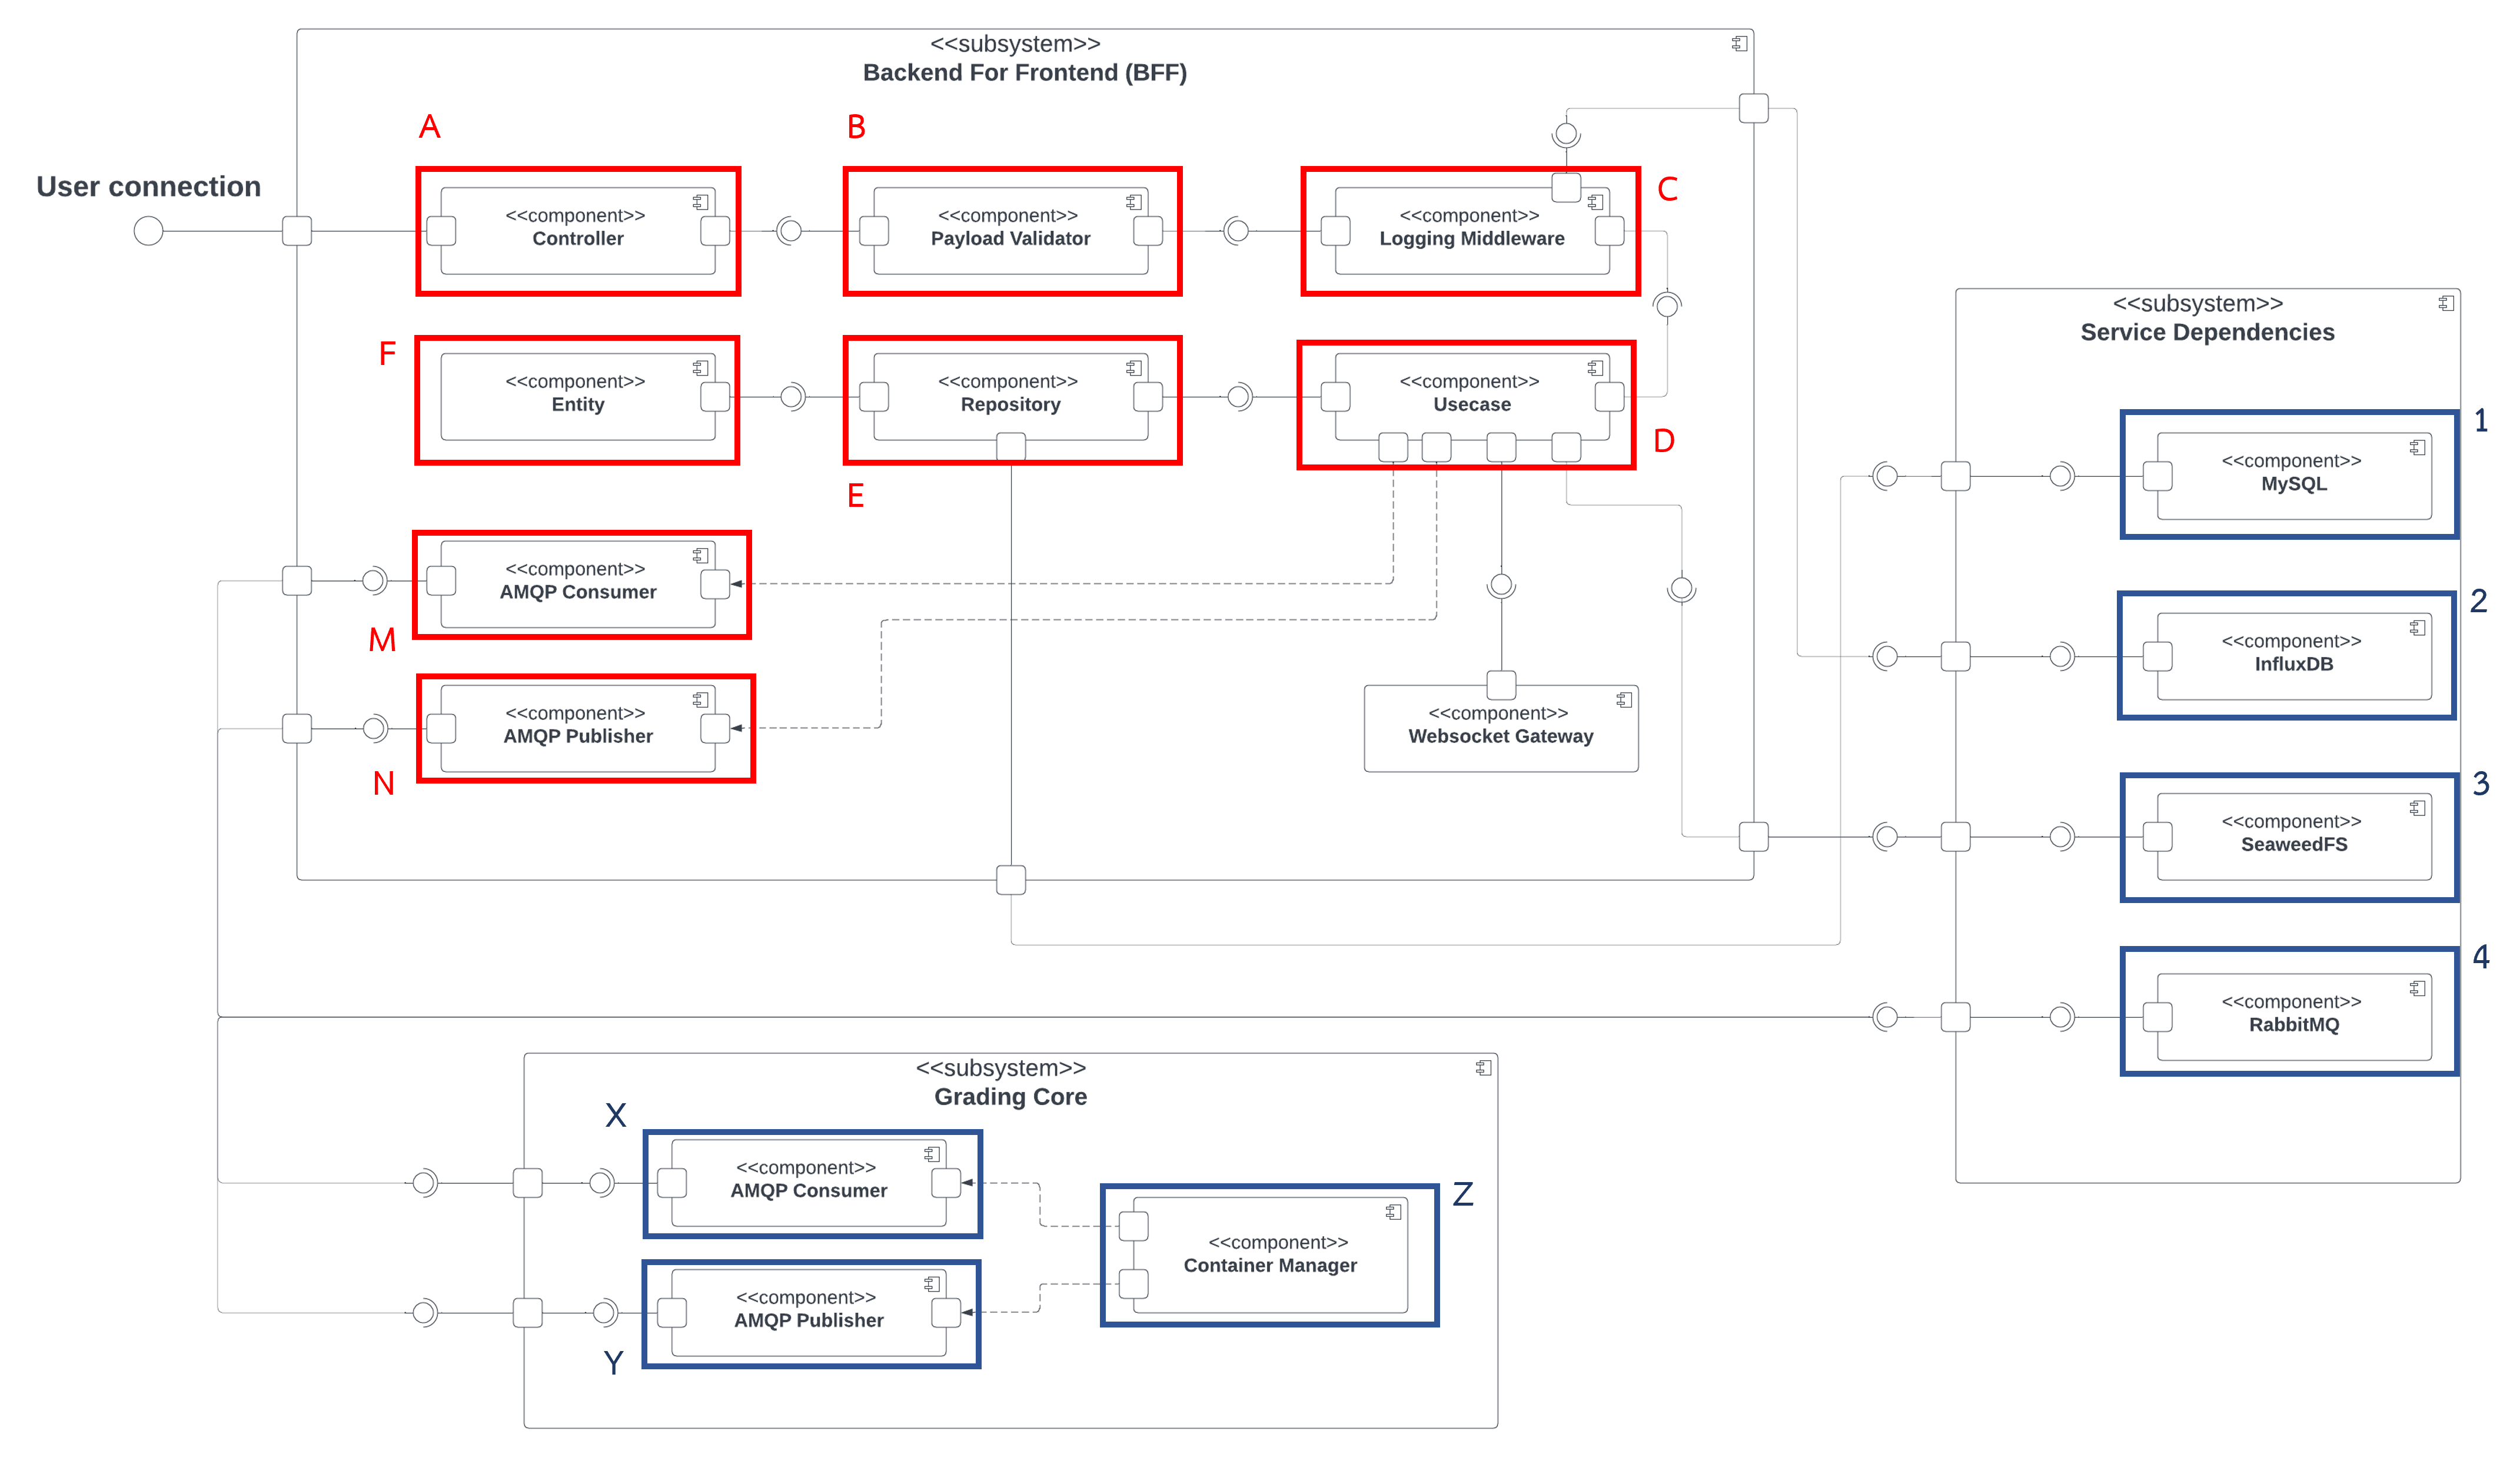
\includegraphics[width=17cm]{figure/diagram/component_v2.png}
            }
                \caption[ภาพแผนผังเเสดงโครงสร้างเเละส่วนประกอบของซอฟต์เเวร์]{แผนภาพเเสดงโครงสร้างเเละส่วนประกอบของซอฟต์เเวร์ วาดด้วย \href{https://lucid.app/}{LucidChart}}
                \label{fig:comp-diagram}
            \end{figure}
        }
        จากแผนภาพในรูปที่~\ref{fig:comp-diagram} องค์ประกอบหลักของระบบซอฟต์แวร์ประกอบไปด้วย 3 ส่วนหรือระบบย่อยดังนี้
        \begin{enumerate}
            \item \textbf{Backend For Frontend} (BFF) คือระบบย่อยหลักทำหน้าที่การประมวลผลการแสดงออกหน้าเว็บไซต์ โดยมีองค์ประกอบดังนี้
            \begin{itemize}
                \item ส่วนแรกที่ผู้ใช้เชื่อมต่อเข้ามายังระบบ คือ \textbf{Controller} (กรอบแดง A) เป็นส่วนที่คอยรับการเชื่อมต่อของผู้ใช้เข้ามาภายในระบบ
                \item Controller จะส่งต่อการทำงานให่อีกองค์ประกอบหนึ่งที่ชื่อ \textbf{Payload Validator} (กรอบแดง B) ซึ่งจะทำการตรวจสอบความถูกต้องของการเชื่อมต่อ (Connection)
                \item การเชื่อมต่อทั้งหมดจะถูกเก็บเป็นสถิติ ผ่านองค์ประกอบที่ชื่อว่า \textbf{Logging Middleware} (กรอบแดง C)
                \item ส่วนประกอบที่ชื่อ \textbf{Usecase} (กรอบแดง D) จะทำหน้าที่ประมวลผลการเรียกขอข้อมูล (Request) จากผู้ใช้
                \item ถ้าหากต้องการจะเข้าถึงฐานข้อมูล ส่วนประกอบที่ชื่อ \textbf{Repository} (กรอบแดง E) จะทำเข้าถึงฐานข้อมูล และหยิบดึง (Query) ข้อมูลส่งกลับให้ผู้ใช้
                \item ข้อมูลที่ถูกดึงจากฐานข้อมูล มีรูปแบบหรือลักษณะ (Format) ที่ถูกนิยามโดยส่วนประกอบที่ชื่อ \textbf{Entity} (กรอบแดง F)
            \end{itemize}
            \item \textbf{Service Dependencies} คือระบบย่อยสำหรับเก็บข้อมูลโดยเฉพาะ ประกอบด้วยองค์ประกอบที่ทำหน้าที่เก็บข้อมูลรูปแบบใดรูปแบบหนึ่ง ประกอบด้วยองค์ประกอบย่อยดังนี้
                \begin{itemize}
                    \item \textbf{MySQL} (กรอบน้ำเงิน 1) เป็นฐานข้อมูลตารางหรือ Relational Database ที่ทำหน้าที่เก็บข้อมูลทั่วไปที่จำเป็นต่อ feature ต่าง ๆ ของซอฟต์แวร์ ตั้งแต่ข้อมูลผู้ใช้ไปจนถึงข้อมูลโจทย์ปัญหา การบ้านหรือข้อสอบทั้งหมด พร้อมทั้งกรณีทดสอบหรือเทสเคส ระบบ BFF เข้าถึงฐานข้อมูลนี้ผ่านองค์ประกอบย่อยชื่อ Repository (กรอบแดง E)
                    \item ตามที่ได้กล่าวไปข้่างต้น ข้อมูลการเชื่อมต่อทั้งหมดจะถูกเก็บเป็นสถิติในองค์ประกอบย่อย Logging Middleware โดยข้อมูลการเชื่อมต่อทั้งหมดนั้นจะถูกนำไปเก็บใน \textbf{InfluxDB} (กรอบน้ำเงิน 2) ซึ่งเป็นฐานข้อมูลประเภทห้วงเวลาหรือ Time-series Database ที่จะเก็บข้อมูลการเชื่อมต่อทั้งหมดนั้นในเป็นช่วงๆ เวลาไป
                    \item ข้อมูลที่เป็นไฟล์ทั้งหมด ไม่ว่าจะเป็นไฟล์ pdf ของโจทย์ (Assignment), ไฟล์ expected input และ output (Test Case) หรือแม้กระทั่งรูปโปรไฟล์ของผู้ใช้ เป็นต้น จะถูกเก็บในระบบบริการไฟล์หรือ File Service หรือ Filer ชื่อ \textbf{SeaweedFS} (กรอบน้ำเงิน 3)
                    \item เนื่องจากระบบซอฟต์แวร์นี้ใช้การ Publish และ Consume ในการแลกเปลี่ยน request และ response ระหว่างระบบย่อย BFF และ Grading Core จึงจำเป็นต้องมี Message Broker ที่จะเก็บพวก message ต่าง ๆ เหล่านี้ ชื่อ \textbf{RabbitMQ} (กรอบน้ำเงิน 4) 
                \end{itemize}
            \item \textbf{Grading Core} คือระบบย่อยสำหรับการประมวลผลและ Compile ไฟล์งานหรือโปรแกรมของผู้ใช้ ที่ส่งเข้ามาในระบบให้ตรวจ
                \begin{itemize} 
                    \item  การรับการเรียกขอ (request) ตรวจงานจากระบบย่อย Backend For Frontend จะทำผ่านองค์ประกอบ \textbf{AMQP Consumer} (กรอบน้ำเงิน X) โดย Consumer นี้จะไปรับคำขอที่ทาง BFF ส่งเข้า RabbitMQ (กรอบน้ำเงิน 4) ผ่าน Publisher ของตัว BFF (กรอบแดง N)
                    \item หลังจากตรวจเสร็จ ก็จะส่งผลลัพธ์ผ่านองค์ประกอบ AMQP Publisher ของ 
                    Grading Core (กรอบนำ้เงิน Y) เข้า RabbitMQ (กรอบน้ำเงิน 4) เพื่อให้องค์ประกอบ AMQP Consumer ที่อยู่ในระบบย่อย BFF (กรอบนำ้เงิน M) Consume ไปเเสดงผลที่หน้าเว็บ
                \end{itemize}
        \end{enumerate}
    \pagebreak
    \subsection{เเผนภาพลำดับการทำงาน}
    %%%%%%%%%%% SEQUENCE DIAGRAM %%%%%%%%%%%
         \hypertarget{seq-diagram1}{
                \begin{figure}[!h]
                \centering
                \fbox{
                    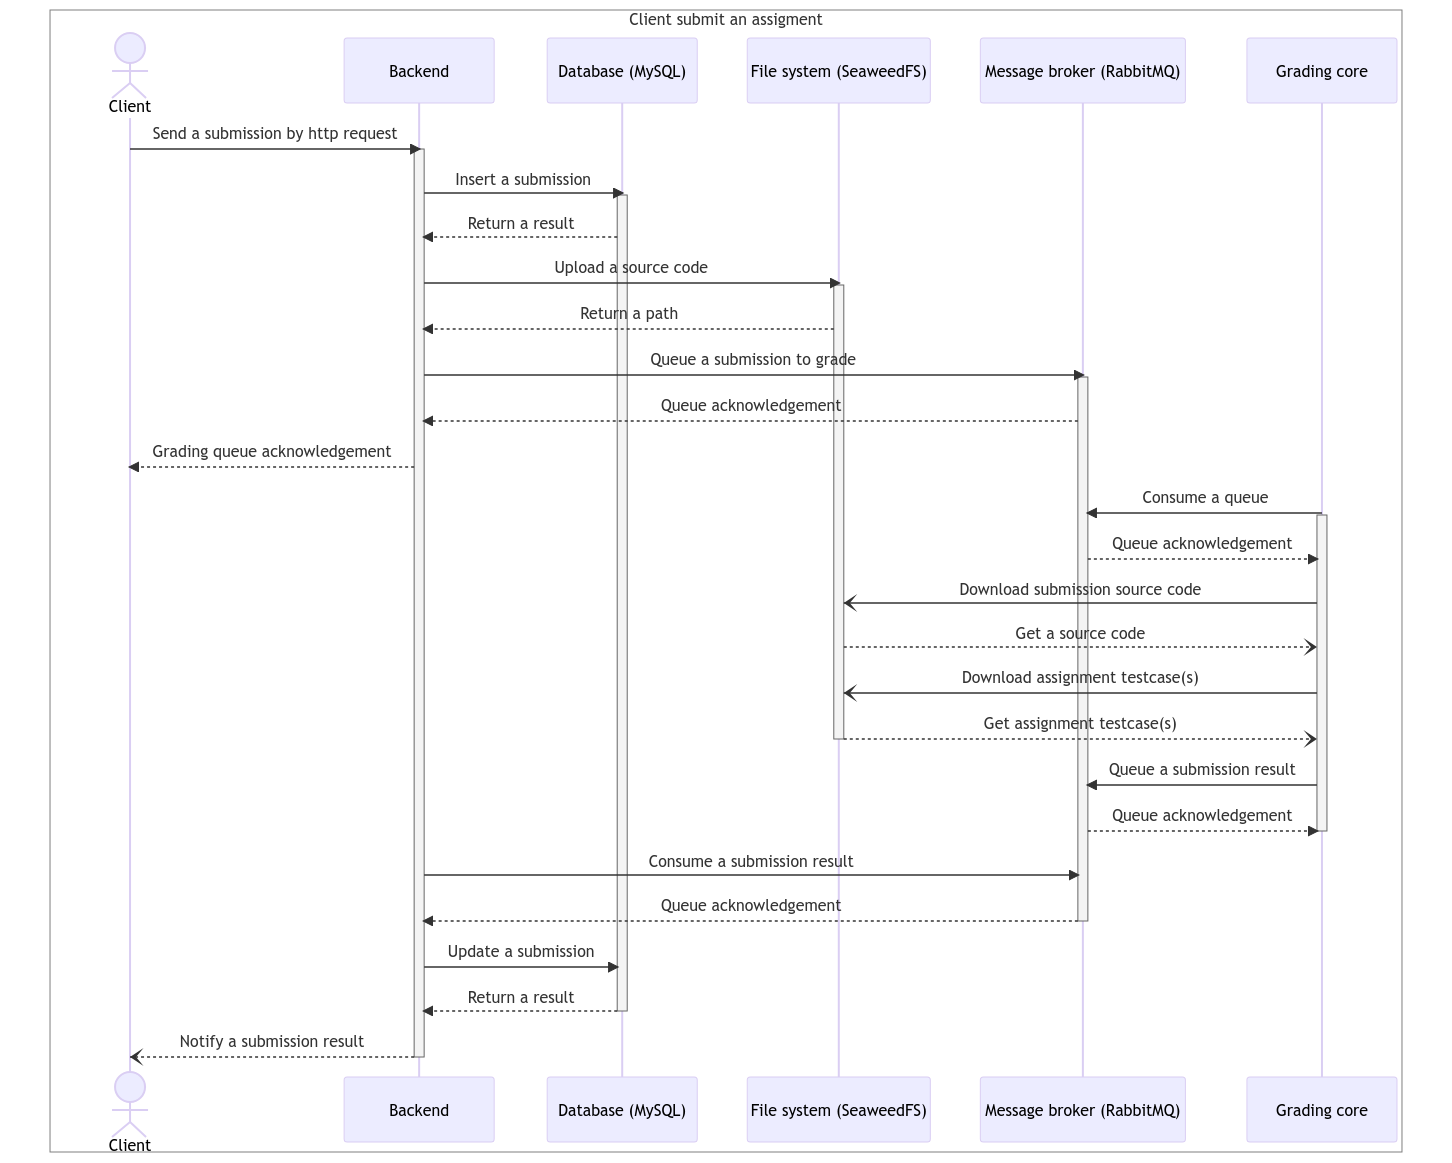
\includegraphics[width=15cm]{figure/diagram/seq-submit_grading-v1.png}
                }
                    \caption[ภาพเเผนภาพลำดับการทำงาน]{เเผนภาพลำดับการทำงานของการส่งโปรเเกรมขึ่้นระบบตรวจ วาดด้วย \href{https://mermaid.js.org/}{Mermaid JS}}
                    \label{fig:seq-diagram1}
                \end{figure}
            }
        \begin{flushleft}
        แผนภาพลำดับการทำงานในรูปที่ \hyperlink{comp-diagram}{3.25} อธิบายกระบวนการทำงานของระบบการตรวจไฟล์งานเขียนโปรแกรมที่ผู้ใช้ส่งเข้ามาให้ตรวจ โดยมีการ actor ดังนี้ (เรียงลำดับขั้นตอน จากบนสุดสู่ล่างสุดของแผนผัง)
        \end{flushleft}
        \begin{itemize}
            \item Client (ผู้ใช้) เริ่มต้นกระบวนการโดยส่งคำขอทาง HTTP ไปยัง Backend เพื่อส่งไฟล์งานเขียนโปรแกรม
            \item Backend (ส่วนหลักของระบบ) รับคำขอและทำการบันทึกไฟล์งานเขียนโปรแกรมลงในฐานข้อมูล MySQL หลังจากนั้นส่งผลการทำงานกลับไปยัง Client พร้อมกับข้อมูลผลการบันทึก
            \item File system (SeaweedFS) ใช้เพื่อเก็บโค้ดของงานและข้อมูลเกี่ยวกับงานต่างๆ เมื่อ Backend อัพโหลดไฟล์งานเขียนให้ File system ก็จะคืน path ที่เก็บไฟล์กลับไปให้ Backend
            \item Message broker (RabbitMQ) มีหน้าที่จัดการการส่งคิวของงานตรวจคะแนนโค้ด หลังจากนั้นส่งการยืนยันการจัดคิวกลับไปยัง Backend แล้วจากนั้น Backend ก็จะส่งการยืนยันต่อไปให้ Client ด้วย
            \item Grading core เป็นส่วนของระบบที่รับผิดชอบในการดำเนินการตรวจคะแนนโค้ด โดยมีกระบวนการดังต่อไปนี้
            \begin{itemize}
                \item Grading core ทำการเช็ค (consume) queue ใน Message broker เพื่อดูว่ามีไฟล์งานเขียนโปรแกรมถูกส่งมาให้ตรวจหรือไม่
                \item Grading core เริ่มต้นกระบวนการโดยการทำการดึงโค้ดของงานและข้อมูลของงานจาก File system
                \item หลังจากที่ทำการตรวจคะแนนเสร็จสิ้น Grading core จะทำการส่งผลการตรวจคะแนนกลับไปยัง Message broker เพื่อจัดคิวการแจ้งผลตรวจคะแนนของงาน
            \end{itemize}
            \item Backend ต่อมาทำการดึงผลการตรวจคะแนนที่ Message broker แจ้งกลับมา และทำการอัพเดทข้อมูลของงานในฐานข้อมูล MySQL พร้อมส่งผลการตรวจคะแนนกลับมา มาแจ้งให้ Client
        \end{itemize}
        \begin{flushleft}
        กระบวนการนี้ช่วยในการจัดการและควบคุมกระบวนการตรวจคะแนนงานเขียนโค้ดของระบบ ให้เป็นระเบียบและมีประสิทธิภาพ มีการใช้ Message broker เพื่อรวมและควบคุมการทำงานของ Grading Core และ Backend ให้ทำงานร่วมกันได้อย่างมีประสิทธิภาพ
        \end{flushleft}
    
    \subsection{แผนผังแสดงโครงสร้างและการนำทางระหว่างหน้าของเว็บไซต์}
    %%%%%%%%%%% NAVIGATION MAP %%%%%%%%%%%
        \hypertarget{nav-map}{
                \begin{figure}[!h]
                \centering
                \fbox{
                    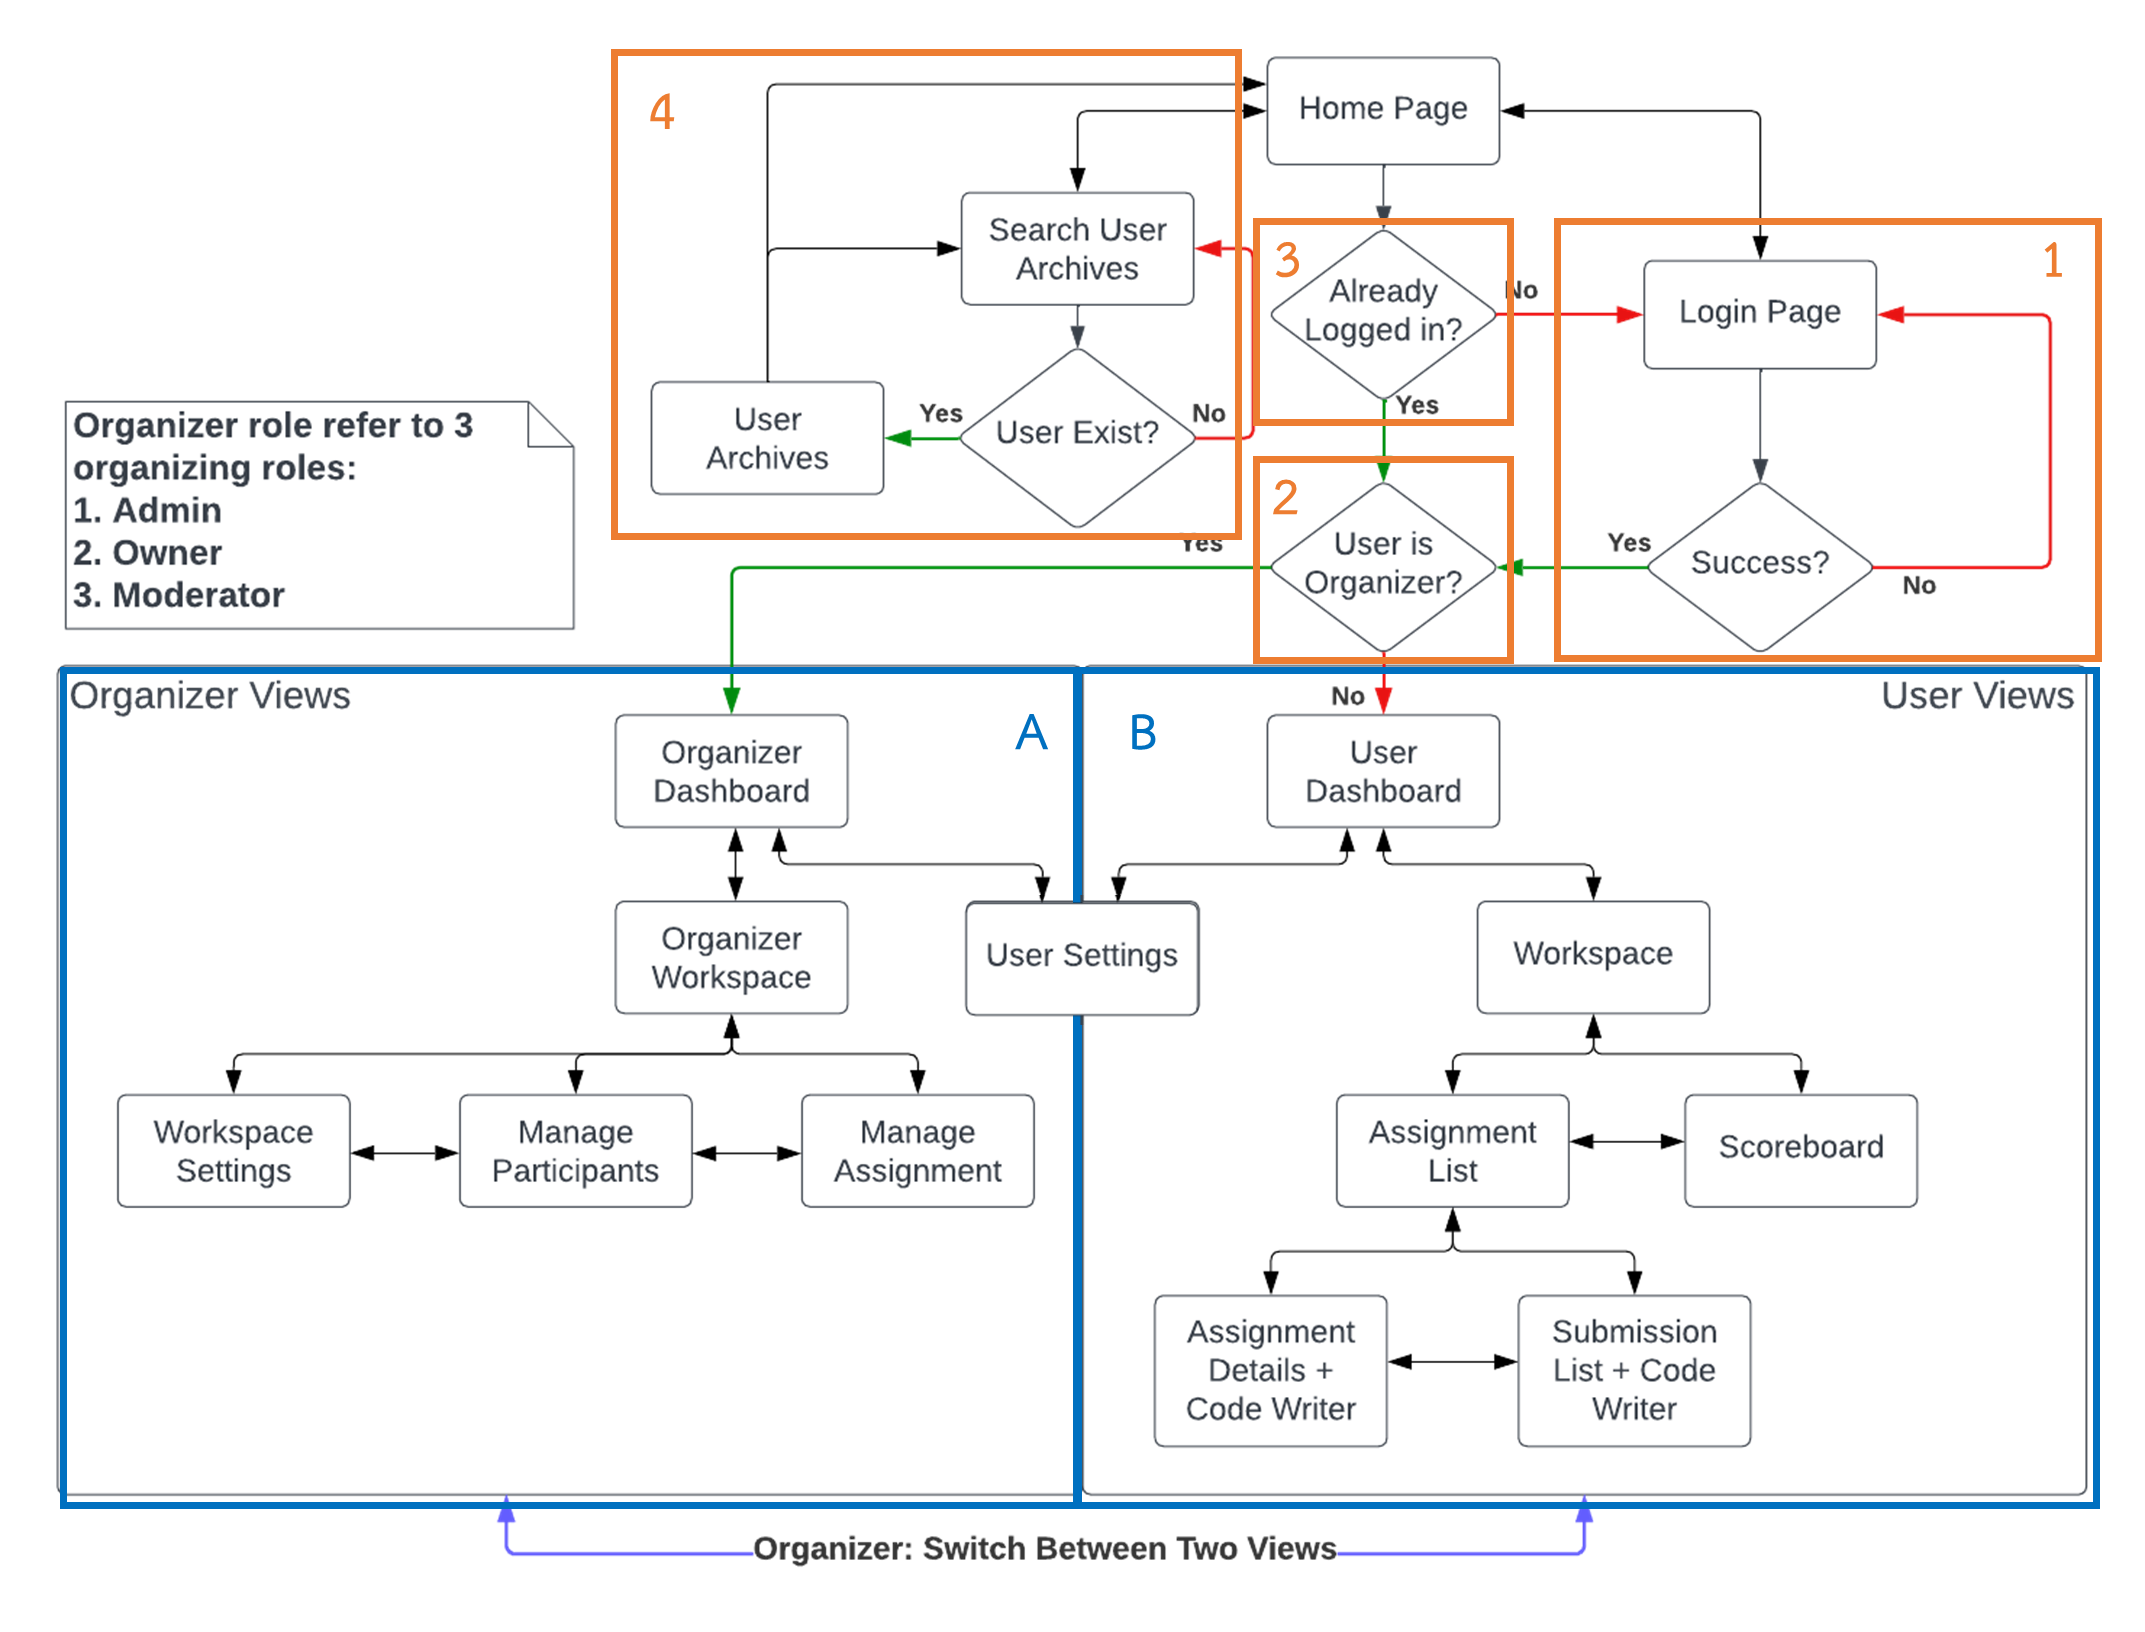
\includegraphics[width=15cm]{figure/diagram/navigation-v2.png}
                }
                    \caption[ภาพแผนผังแสดงโครงสร้างและการนำทางระหว่างหน้าของเว็บไซต์]{แผนผังแสดงโครงสร้างและการนำทางระหว่างหน้าของเว็บไซต์ วาดด้วย \href{https://lucid.app/}{LucidChart}}
                    \label{fig:nav-map}
                \end{figure}
            }
        \begin{flushleft}
        จากรูปที่ \hyperlink{nav-map}{3.26} ข้างต้น เป็นแผนผังโครงสร้างของหน้าเว็บของซอฟต์แวร์ของเรา และการนำทาง ไปมาระหว่างแต่ละหน้าเว็บของซอฟต์แวร์
        \end{flushleft}
        \begin{flushleft}
        เริ่มต้นจากหน้าแรก (Home page) ของซอฟต์แวร์เรา จากหน้าแรกก็จะสามารถเข้าถึงได้สองหน้า โดยไม่ต้องเข้าสู่ระบบคือหน้าค้นทะเบียนประวัติผู้ใช้เก่า (Search User Archives) (กรอบที่ 4 \hyperlink{nav-map}{3.26}) ซึ่งเป็นจะเป็นหน้าสำหรับกรอกรหัสหรือชื่อของผู้ใช้ที่ต้องการจะค้นทะเบียนประวัติ ถ้าหากค้นแล้วไม่พบผู้ใช้คนดังกล่าว ก็จะถูกตีกลีบไปที่หน้าเดิม แต่ถ้าค้นเจอก็จะถูกนำพามาหน้าแสดงข้อมูลของผู้ใช้ที่ได้ค้นไปเมื่อครู่ (ตรงกับหน้าจอในรูปที่ \hyperlink{ui-archive1}{3.22})
        \end{flushleft}
        \begin{flushleft}
        จากหน้าแรก ถ้ากดปุ่ม “Login” ก็จะนำพาผู้ใช้เข้าสู่ระบบยืนยันตัวตน ถ้าหากผู้ใช้ยังไม่ได้เข้าสู่ระบบหรือไม่ได้มี session อยู่ในระบบ ณ ตอนนั้น ก็จะถูกนำพาไปหน้าเข้าสู่ระบบ (Login Page) (กรอบที่ 1 ในรูปที่ \hyperlink{nav-map}{3.26}) ถ้าหากกรอกข้อมูลผิดอาทิเช่น ชื่อผู้ใช้/อีเมล รหัสผ่าน เป็นต้น ก็จะถูกนำทางกลับไปเข้าสู่หน้าเข้าสู่ระบบหน้าเดิม จนกว่าจะกรอกข้อมูลถูกต้อง
        \end{flushleft}
        \begin{flushleft}
        ในทางกลับกันถ้าหากผู้ใช้เข้าสู่ระบบแล้ว หรือมี session อยู่ในระบบ ณ ตอนนั้น ก็จะถูกนำพาเข้าสู่แผงควบคุมทันที (กรอบที่ 3 ในรูปที่ \hyperlink{nav-map}{3.26}) ทั้งนี้ก็ขึ้นอยู่กับบทบาท (role) ของผู้ใช้ว่าเป็น Organizer (หรือบทบาทผู้ดูแลทั้งสามตำแหน่ง: Admin, Owner, และ Moderator ตาม requirements) หรือเป็นผู้ใช้ทั่วไป (หรือ Registered User, Student, Attendee ตาม requirements) บทบาทผู้ใช้แต่ละบทบาท จะถูกนำพาไปสู่รูปแบบแผงควบคุมคนละแบบ (กรอบที่ 2)  
        \end{flushleft}
        \begin{flushleft}
        ถ้าหากเป็น Organizer ก็จะนำพาไปแผงควบคุมที่ในมุมมองของ Organizer (Organizer view) (กรอบ A ในรูปที่ \hyperlink{nav-map}{3.26}) ซึ่งสอดคล้องกับ ส่วนประสานผู้ใช้รูปที่ \hyperlink{ui-org-dashboard1}{3.11} โดยจากแผงควบคุมของ Organizer ก็จะสามารถจะเข้าถึง หน้าตั้งค่าของบัญชีตนเอง (User Settings) และห้องเรียนหรือกลุ่มเรียน (Organizer workspace) ทั้งหมดที่ Organizer คนนั้น ๆ เป็นเจ้าของหรือเข้าถึงได้ หลังจากกดเลือกห้องเรียนหรือกลุ่มเรียนเข้ามาแล้ว ก็จะถูกนำพาเข้ามาหน้าหลักของห้องเรียนหรือกลุ่มเรียนนั้น ๆ (ตรงกับหน้าจอในรูปที่ \hyperlink{ui-org-assign1}{3.13}) ซึ่งสามารถเข้าถึงหน้าตั้งค่าห้องเรียนหรือกลุ่มเรียน (Workspace Settings), หน้าบริหารจัดการสมาชิกห้องเรียนหรือกลุ่มเรียน (Manage Participants), และหน้าบริหารจัดการภาระงาน (Manage Assignment) 
        \end{flushleft}
        \begin{flushleft}
        ถ้าผู้ใช้ไม่ได้มีบทบาทเป็น Organizer แต่เป็นผู้ใช้ทั่วไป (User) ก็จะนำพามาแผงควบคุมในมุมมองของ User (User View) (กรอบ B ในรูปที่ \hyperlink{nav-map}{3.26}) ซึ่งตรงกับรูปหน้าจอในรูปที่ \hyperlink{ui-dashboard1}{3.4} จากหน้าแผงควบคุมดังกล่าว User สามารถจะเข้าถึง หน้าตั้งค่าของบัญชีตนเอง (User Settings) และห้องเรียนหรือกลุ่มเรียน (Workspace) ทั้งหมดที่ User คนนั้น ๆ ได้เข้าร่วมหรือถูกยัดเข้า หลังจากกดเลือกห้องเรียนหรือดักลุ่มเรียนเข้ามาแล้ว ก็จะถูกนำทางมาหน้าหลักของห้องเรียนหรือกลุ่มเรียนนั้น ๆ ซึ่งก็คือหน้าจอแสดงรายการภาระงาน (Assignment List) ทั้งหมดในกลุ่มเรียนหรือห้องเรียนนั้น ๆ (เป็นหน้าจอของรูปที่ \hyperlink{ui-assign1}{3.12}) นอกจากหน้ารายการภาระงานแล้ว User ก็สามารถกดไปดูตารางคะแนน (Scoreboard) ของห้องเรียนหรือกลุ่มเรียนนั้นได้ด้วย 
        \end{flushleft}
        \begin{flushleft}
        ถ้าผู้ใช้ทั่วไปหรือ User กดเลือกภาระงานในหน้ารายการแสดงภาระงาน ก็จะถูกนำพาไปหน้าเขียนโปรแกรมซึ่งประกอบแผงเขียนโปรแกรม (Code Writer) กับส่วนแสดงเนื้อหาโจทย์ (Assignment Details) หน้าจอดังกล่าวตรงกับหน้าจอในรูปที่ \hyperlink{ui-code1}{3.20} ผู้ใช้สามารถที่จะเปลี่ยนแผงแสดงเนื้อหาโจทย์เป็นแผงแสดงรายการการส่งโปรแกรมตรวจ (Submission List ได้) ซึ่งตรงกับหน้าจอในรูปที่ \hyperlink{ui-code2}{3.21}
        \end{flushleft}
        \begin{flushleft}
        ข้อที่ควรรู้เพิ่มเติมคือ ถ้าหากผู้ใช้มีบทบาทเป็น Organizer ผู้ใช้จะสามารถสับเปลี่ยนมุมมอง (Switch View) จาก Organizer เป็น User หรือ User เป็น Organizer ได้ ด้วยปุ่ม “Switch to Normal Mode” หรือ “Switch to Organizer Mode” ตามลำดับ (มีให้เห็นในรูปที่ \hyperlink{ui-org-dashboard1}{3.11} และ \hyperlink{ui-assign1}{3.12} ตรงมุมขวาบน)
        \end{flushleft}
    \pagebreak
\newpage
%%%%%%%%%%%%%%%%%%%%%%%%%%%%%%%%%%%%%%%%%%%%%%%%%%%%%%%%%%%%%%
%%%%%%%%%%%%%%%%%%%% Experiments %%%%%%%%%%%%%%%%%%%%%%%%%%%%%
%%%%%%%%%%%%%%%%%%%%%%%%%%%%%%%%%%%%%%%%%%%%%%%%%%%%%%%%%%%%%%%
% \chapter{ผลการดำเนินงาน}

% \emph{หัวข้อต่าง ๆ ในแต่ละบทเป็นเพียงตัวอย่างเท่านั้น หัวข้อที่จะใส่ในแต่ละบทขึ้นอยู่กับโปรเจคของนักศึกษาและอาจารย์ที่ปรึกษา}

% % ตัวอย่างการใส่อ้างอิงที่มา -> \cite{hypersense} ถ้าต้องการใส่แหล่งอ้างอิงมากกว่า 1 ให้ทำดังนี้ -> \cite{hypersense,bworld} 

% You can title this chapter as \textbf{Preliminary Results} ผลการดำเนินงานเบื้องต้น or \textbf{Work Progress} ความก้าวหน้าโครงงาน for the progress reports. Present implementation or experimental results here and discuss them.
% ใส่เฉพาะหัวข้อที่เกี่ยวข้องกับงานที่ทำ 

% \section{ประสิทฺธิภาพการทำงานของระบบ} 
% \section{ความพึงพอใจการใช้งาน}
% \section{การวิเคราะห์ข้อมูลและผลการทดลอง}

%%%%%%%%%%%%%%%%%%%%%%%%%%%%%%%%%%%%%%%%%%%%%%%%%%%%%%%%%%%%%%%
%%%%%%%%%%%%%%%%%%%% Conclusions %%%%%%%%%%%%%%%%%%%%%%%%%%%%%
%%%%%%%%%%%%%%%%%%%%%%%%%%%%%%%%%%%%%%%%%%%%%%%%%%%%%%%%%%%%%%%
% \chapter{บทสรุป}


% \emph{หัวข้อต่าง ๆ ในแต่ละบทเป็นเพียงตัวอย่างเท่านั้น หัวข้อที่จะใส่ในแต่ละบทขึ้นอยู่กับโปรเจคของนักศึกษาและอาจารย์ที่ปรึกษา}



% This chapter is optional for proposal and progress reports but 
% is required for the final report.

% \section{สรุปผลโครงงาน}
% สรุปว่าโครงงานบรรลุตามวัตถุประสงค์ที่ตั้งไว้หรือไม่ อย่างไร 

% \section{ปัญหาที่พบและการแก้ไข}
% State your problems and how you fixed them.

% \section{ข้อจำกัดและข้อเสนอแนะ}
% ข้อจำกัดของโครงงาน What could be done in the future to make your projects better.

%%%%%%%%%%%%%%%%%%%%%%%%%%%%%%%%%%%%%%%%%%%%%%%%%%%%%%%%%%%%%%%
%%%%%%%%%%%%%%%%%%%% Bibliography %%%%%%%%%%%%%%%%%%%%%%%%%%%%%
%%%%%%%%%%%%%%%%%%%%%%%%%%%%%%%%%%%%%%%%%%%%%%%%%%%%%%%%%%%%%%%

%%%% Comment this in your report to show only references you have
%%%% cited. Otherwise, all the references below will be shown.
%\nocite{*}
%% Use the kmutt.bst for bibtex bibliography style 
%% You must have cpe.bib and string.bib in your current directory.
%% You may go to file .bbl to manually edit the bib items.

% Sept, 2021 by Thanin
% improve url breaks to prevent unnecessary big white spaces in some cases
\makeatletter
\g@addto@macro{\UrlBreaks}{\UrlOrds}
\makeatother
% 

\bibliographystyle{kmutt}
% \bibliography{example/string,example/string2,example/cpe}
\bibliography{codern}

%%%%%%%%%%%%%%%%%%%%%%%%%%%%%%%%%%%%%%%%%%%%%%%%%%%%%%%%%%%%%%%
%%%%%%%%%%%%%%%%%%%%%%%% Appendix %%%%%%%%%%%%%%%%%%%%%%%%%%%%%
%%%%%%%%%%%%%%%%%%%%%%%%%%%%%%%%%%%%%%%%%%%%%%%%%%%%%%%%%%%%%%%
% \appendix{ชื่อภาคผนวกที่ 1}
% \noindent{\large\bf ใส่หัวข้อตามความเหมาะสม} \\

% This is where you put hardware circuit diagrams, detailed experimental data in tables or source codes, etc.. \\ \bigskip


%  \begin{figure}[!h]
% \caption{This is the figure x11 ทดสอบ จาก \href{https://www.google.com} {https://www.google.com}}\label{fig:x1}
% \end{figure}


% This appendix describes two static allocation methods for fGn (or fBm)
% traffic. Here, $\lambda$ and $C$ are respectively the traffic arrival
% rate and the service rate per dimensionless time step. Their unit are
% converted to a physical time unit by multiplying the step size
% $\Delta$. For a fBm self-similar traffic source,
% Norros~\cite{norros95} provides its EB as
% \begin{equation}\label{eq:norros}
%   C = \lambda + (\kappa(H)\sqrt{-2\ln\epsilon})^{1/H}a^{1/(2H)}x^{-(1-H)/H}\lambda^{1/(2H)}
% \end{equation}
% where $\kappa(H) = H^H(1-H)^{(1-H)}$. Simplicity in the calculation is
% the attractive feature of (\ref{eq:norros}).

% The MVA technique developed in~\cite{kim01} so far provides the most
% accurate estimation of the loss probability compared to previous
% bandwidth allocation techniques according to simulation results.
% Consider a discrete-time queueing system with constant service rate
% $C$ and input process $\lambda_n$ with $\mathbb{E}\{\lambda_n\} =
% \lambda$ and $\mathrm{Var}\{\lambda_n\} = \sigma^2$.  Define $X_n \equiv
% \sum_{k=1}^n \lambda_k - Cn$.  The loss probability due to the MVA
% approach is given by
% \begin{equation}\label{eq:loss_mva}
%   \varepsilon \approx \alpha e^{-m_x/2}
% \end{equation}
% where
% \begin{equation}\label{eq:mx}
% m_x = \min_{n \geq 0} \frac{((C-\lambda)n + B)^2}{\mathrm{Var}\{X_n\}} =
% \frac{((C-\lambda)n^\ast + B)^2}{\mathrm{Var}\{X_{n^{\ast}}\}}
% \end{equation} 
% and 
% \begin{equation}\label{eq:alpha}
%   \alpha =
%   \frac{1}{\lambda\sqrt{2\pi\sigma^2}}\exp\left(\frac{(C-\lambda)^2}{2\sigma^2}\right)
%   \int_C^\infty (r-C)\exp\left(\frac{(r-\lambda)^2}{2\sigma^2}\right)\, dr
% \end{equation}
% For a given $\varepsilon$, we numerically solve for $C$ that satisfies
% (\ref{eq:loss_mva}). Any search algorithm can be used to do the task.
% Here, the bisection method is used.  

% Next, we show how $\mathrm{Var}\{X_n\}$ can be determined.  Let
% $C_{\lambda}(l)$ be the autocovariance function of $\lambda_n$.  The
% MVA technique basically approximates the input process $\lambda_n$
% with a Gaussian process, which allows $\mathrm{Var}\{X_n\}$ to be
% represented by the autocovariance function.  In particular, the
% variance of $X_n$ can be expressed in terms of $C_{\lambda}(l)$ as
% \begin{equation}
%   \mathrm{Var}\{X_n\} = nC_{\lambda}(0) + 2\sum_{l=1}^{n-1} (n-l)C_{\lambda}(l)
% \end{equation} 
% Therefore, $C_{\lambda}(l)$ must be known in the MVA technique, either
% by assuming specific traffic models or by off-line analysis in case of
% traces.  In most practical situations, $C_{\lambda}(l)$ will not be
% known in advance, and an on-line measurement algorithm developed
% in~\cite{eun01} is required to jointly determine both $n^\ast$ and
% $m_x$. For fGn traffic, $\mathrm{Var}\{X_n\}$ is equal to $\sigma^2
% n^{2H}$, where $\sigma^2 = \mathrm{Var}\{\lambda_n\}$, and we can find
% the $n^\ast$ that minimizes (\ref{eq:mx}) directly. Although $\lambda$
% can be easily measured, it is not the case for $\sigma^2$ and $H$.
% Consequently, the MVA technique suffers from the need of prior
% knowledge traffic parameters.


%%%%%%%%%%%%%%%%%%%%%%%%%%%%%%%%%%%%%%%%%%%%%%%%%%%%%%%%%%
%%%%%%%%%%%%%%% The 2nd appendix %%%%%%%%%%%%%%%%%%%%%%%%%%
%%%%%%%%%%%%%%%%%%%%%%%%%%%%%%%%%%%%%%%%%%%%%%%%%%%%%%%%%%
% \appendix{ชื่อภาคผนวกที่ 2}
% \noindent{\large\bf ใส่หัวข้อตามความเหมาะสม} \\


%  \begin{figure}[!h]
% \caption{This is the figure x11 ทดสอบ จาก \href{https://www.google.com} {https://www.google.com}}\label{fig:x1}
% \end{figure}

% Next, we show how $\mathrm{Var}\{X_n\}$ can be determined.  Let
% $C_{\lambda}(l)$ be the autocovariance function of $\lambda_n$.  The
% MVA technique basically approximates the input process $\lambda_n$
% with a Gaussian process, which allows $\mathrm{Var}\{X_n\}$ to be
% represented by the autocovariance function.  In particular, the
% variance of $X_n$ can be expressed in terms of $C_{\lambda}(l)$ as
% \begin{equation}
%   \mathrm{Var}\{X_n\} = nC_{\lambda}(0) + 2\sum_{l=1}^{n-1} (n-l)C_{\lambda}(l)
% \end{equation} 

% \noindent{\large\bf Add more topic as you need} \\

% Therefore, $C_{\lambda}(l)$ must be known in the MVA technique, either
% by assuming specific traffic models or by off-line analysis in case of
% traces.  In most practical situations, $C_{\lambda}(l)$ will not be
% known in advance, and an on-line measurement algorithm developed
% in~\cite{eun01} is required to jointly determine both $n^\ast$ and
% $m_x$. For fGn traffic, $\mathrm{Var}\{X_n\}$ is equal to $\sigma^2
% n^{2H}$, where $\sigma^2 = \mathrm{Var}\{\lambda_n\}$, and we can find
% the $n^\ast$ that minimizes (\ref{eq:mx}) directly. Although $\lambda$
% can be easily measured, it is not the case for $\sigma^2$ and $H$.
% Consequently, the MVA technique suffers from the need of prior
% knowledge traffic parameters. 

\end{document}
